\chapter{R\&D for Future Solar Neutrino Experiments}
\label{ch:wbls}

Real-time neutrino detectors have frequently functioned on the basis of detecting optical photons produced as energetic charged particles deposit energy in a target medium
Historically, these detectors have progressed from detecting Cherenkov~\cite{cherenkov} light in water targets to detecting scintillation~\cite{birks} light in organic liquid scintillator targets.
This was driven by the desire to detect low energy solar neutrinos, such as the CNO or $pp$ neutrino fluxes, where the interactions would typically fall below the Cherenkov threshold in water, and hence go undetected.
The ability to detect these low energy interactions with scintillators comes with a notable downside: scintillation light, being isotropic, does not carry the directional information of Cherenkov light.
Other notable differences between Cherenkov and scintillation light are summarized in \Cref{tab:chervsscint}.

\begin{table}
\newcolumntype{C}{>{\centering\arraybackslash}X}
\begin{tabularx}{\textwidth}{CC}
Cherenkov & Scintillation \\
\hline
\hline
Directional & Isotropic\\
\hline
Very well understood  & Strong dependence on material properties  \\
\hline
Good shower/MIP separation & Reasonable particle ID  \\
\hline
Minimum energy threshold for light production & No energy threshold for light production  \\
\hline
Low light yield & High light yield results in lower detector threshold and improved energy resolution \\
\hline
Occurs in all dielectric materials, some with very good optical properties & Scintillating materials tend to have substantially shorter attenuation lengths  \\
\hline
Cost-effective & More expensive materials \\
\end{tabularx}
\caption{Comparison of Cherenkov and scintillation light in the context of optical particle detection.}
\label{tab:chervsscint}
\end{table}

Scintillators do, however, also produce Cherenkov light. 
The much higher photon yields of scintillators (approximately 50 times more scintillation photons than Cherenkov photons per MeV in {\labppo}) typically makes the remaining Cherenkov photons quite difficult to detect.
This is further complicated by scintillator optical attenuation and scattering lengths being small relative to neutrino detector sizes, which means many of the Cherenkov photons will be absorbed or scattered, further reducing the directional information available.
The ability to identify these remaining Cherenkov photons would allow future detectors to recover directionality in events above the Cherenkov energy threshold, while simultaneously being sensitive to lower energy interactions through scintillation light.

Directional information is manifestly useful when detecting solar neutrinos, as the elastic scatter (ES) interaction channel produces final state electrons highly correlated with the neutrino direction. 
As the direction of solar neutrinos is away from the Sun, and no backgrounds are expected to be correlated with the solar direction, solar neutrinos are thus relatively easy to identify. 
This directional correlation is not only useful for measurements of solar neutrinos, however. Searches for neutrinoless double beta decay would benefit from rejection of the directional solar neutrino signal, which is the dominant background in experiments such as {\snop}~\cite{snop}.

In general, the identification of Cherenkov photons in a scintillator can be done in three ways:
\begin{itemize}
\item Wavelength:  Cherenkov and scintillation light have different emission spectra (\Cref{fig:optics}). The very broad Cherenkov spectrum could be selectively detected with optical filters that block scintillation light, or by detectors sensitive only to long wavelength photons.
\item Intensity: Cherenkov photons are not isotropic in space, and, with sufficiently dim scintillation light, should have a typical ``Cherenkov ring'' geometry that can be identified on top of an isotropic scintillation background.
\item Timing: Cherenkov emission is very fast, on the order of tens of picoseconds~\cite{cherenkov}, while scintillation light, originating from molecular de-excitation, is typically delayed by 1-10~ns~\cite{birks} and emitted with a profile of exponential time constants of a few to hundreds of nanoseconds.
\end{itemize}

\begin{figure}
\centering
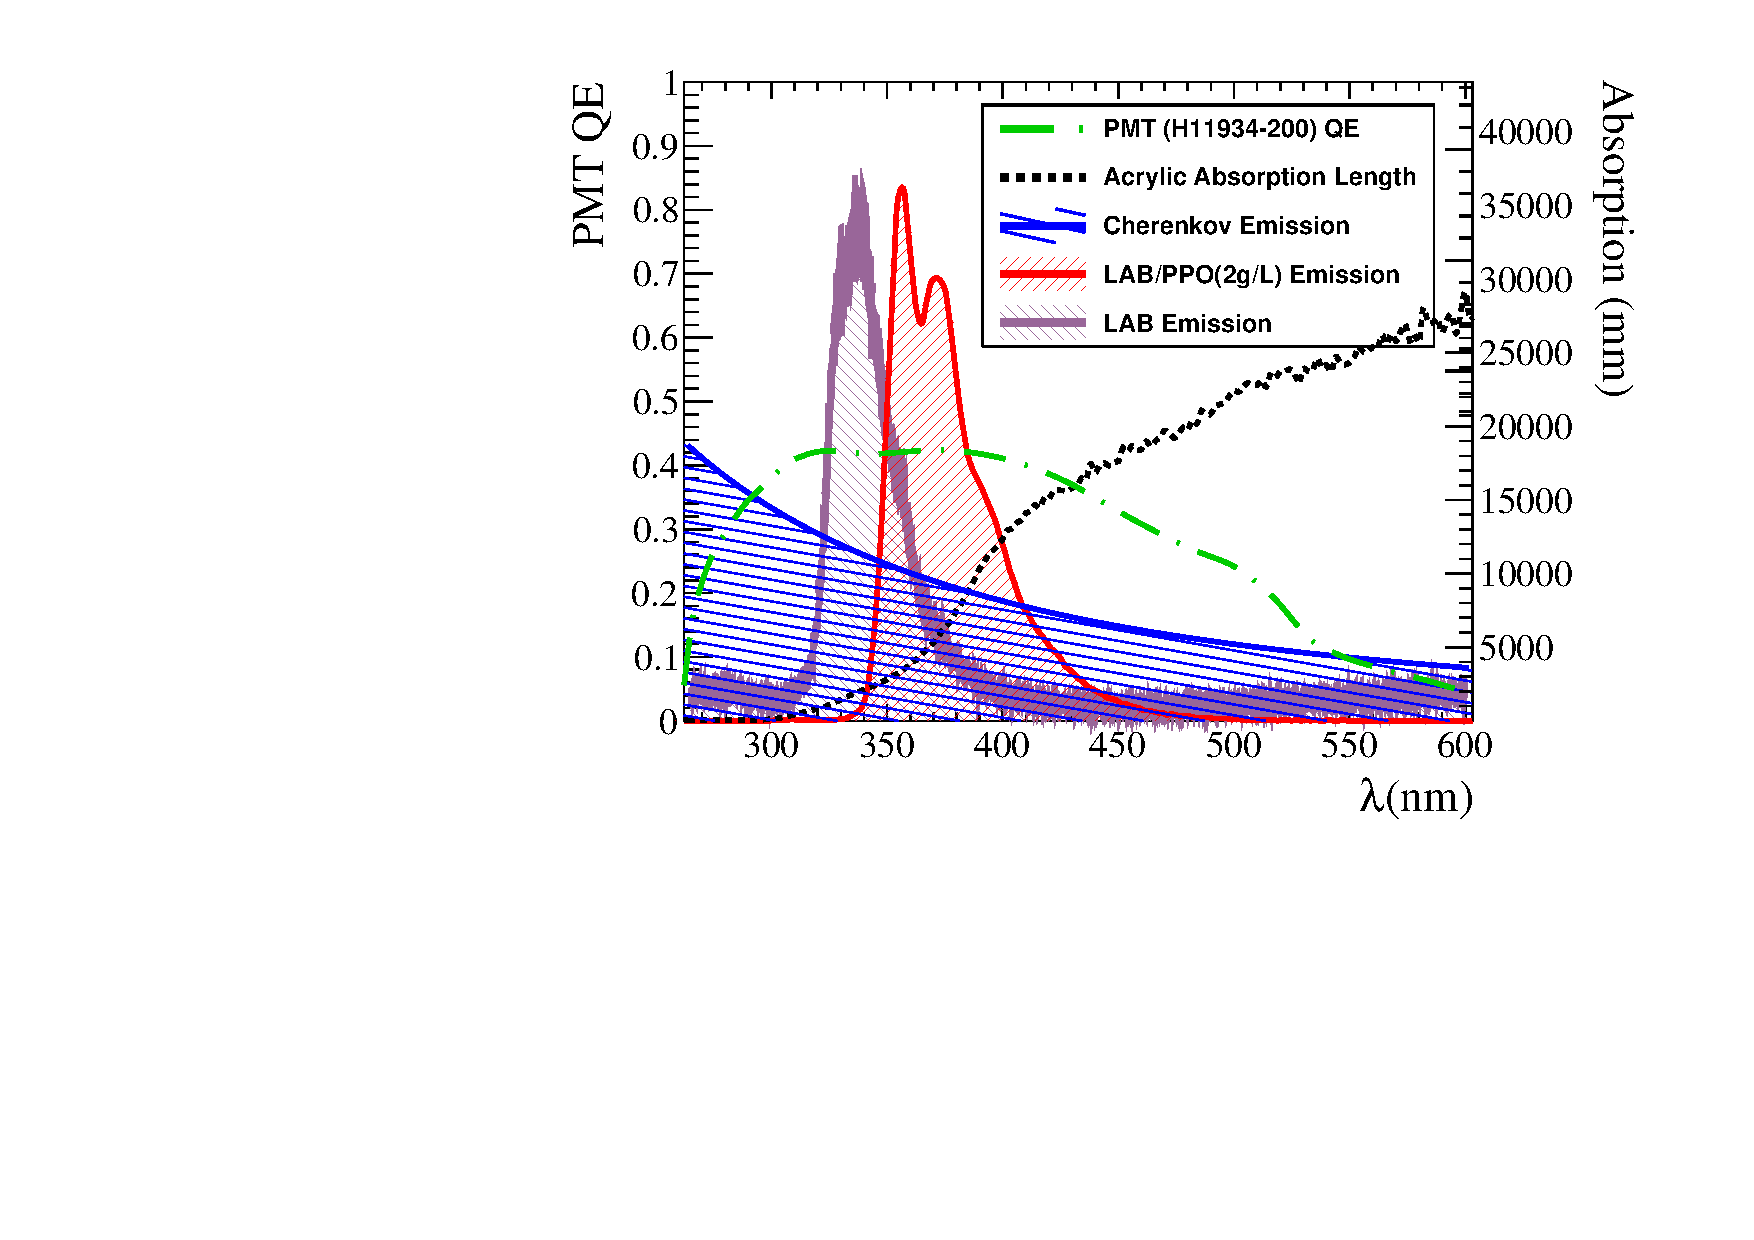
\includegraphics[width=.8\textwidth]{optics.pdf}
\caption{\label{fig:optics} PMT H11934 quantum efficiency~\cite{h11934} and UVT acrylic absorption length compared to the Cherenkov and scintillation emission spectra for pure LAB~\cite{lab_emission} and LAB loaded with 2~g/L PPO~\cite{snop_private}. The normalization of the emission spectra are shown in arbitrary units. Figure from~\cite{chess_nim}.}
\end{figure}

Each option has the potential to enhance Cherenkov photon detection, but each comes with a cost.
Detection-based on wavelength requires expensive optical filters and complicated geometries to avoid losing photons to attenuation.
Intensity-based detection requires that the scintillation intensity be low enough that the Cherenkov topology is still identifiable by contrast.
The recent development of water-based liquid scintillator (WbLS)~\cite{wbls} was in part motivated by the goal of optimizing this balance with a tunable scintillation intensity.
Finally, timing-based detection likely requires very fast (on the order of 100~ps) photon detectors, which can be very expensive.
Traditionally-used large PMTs typically have worse than nanosecond time precision, making Cherenkov light identification in a scintillation medium extremely difficult.
Smaller PMTs~\cite{h11934} can achieve timing precision of $\lesssim$ 300~ps and new micro-channel plate (MCP) photodetector technology~\cite{mcp, lappd, lappd2} can achieve  $\lesssim$ 100~ps.


This chapter describes the CHErenkov / Scintillation Separation (CHESS) experiment~\cite{chess_nim} developed as a part of this thesis, which aims to explore the intensity and timing methods of identifying Cherenkov photons in liquid scintillators. 
Development of CHESS was driven by the recent development of WbLS which allows both the scintillation light yield and timing profile of the target material to be tuned to maximize sensitivity to Cherenkov photons.  
In particular, low scintillator fraction WbLS, from 1\% to 5\% scintillator, is of interest here. 
Being mostly water, this material should have better attenuation characteristics than a pure scintillator, maximizing the likelihood of Cherenkov photons arriving unhindered to a photon detector, and should also have only fractions of scintillation photon yield of pure scintillators, making intensity-based identification of Cherenkov photons a possibility.
CHESS can also explore the potential for Cherenkov photon detection in more traditional scintillators, such as {\labppo}.

\section{The CHESS Detector}\label{s:desc}

A schematic of CHESS is shown in \Cref{fig:timing-setup}.  
An acrylic target vessel is viewed by an array of small, fast PMTs. 
The setup is designed to detect either cosmic muons or events from deployed radioactive sources.  
The primary ring-imaging measurement is performed using through-going muons.  
Vertical-going events are selected via 1-cm diameter coincidence tags above and below the target volume, ensuring a population of events with known orientation and thus a known expectation for the position of the Cherenkov ring. 
The muons produce Cherenkov and scintillation light in the target material, which is detected on the PMT array. 

The apparatus was constructed such that direct Cherenkov light from vertical muons falls on a distinct radial grouping of PMTs, forming a clear ring in the PMT array.
This yields two distinct groups of PMTs by construction: those with only scintillation photons and those with both scintillation and Cherenkov photons. 
Because Cherenkov light is known to be prompt, the earliest hits on any particular PMT can be identified as being caused by either Cherenkov or scintillation photons, depending on the radial position of the PMT.
Therefore, comparing the distribution of first-photon hit times from each radial grouping of PMTs allows one to compare prompt scintillation photons to prompt Cherenkov photons, and one can determine a time cut that results in the best sensitivity to Cherenkov photons.
The total charge collected by each radial group of PMTs also informs the intensity of the Cherenkov photons relative to scintillation photons.

\begin{figure}
\centering
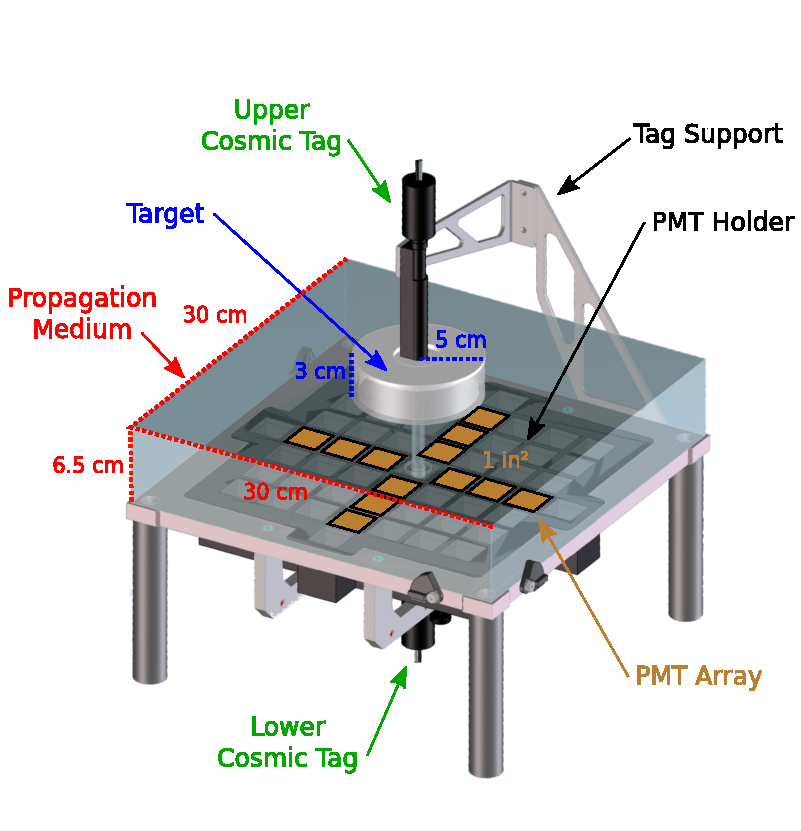
\includegraphics[width=0.54\columnwidth]{timing-schematic}
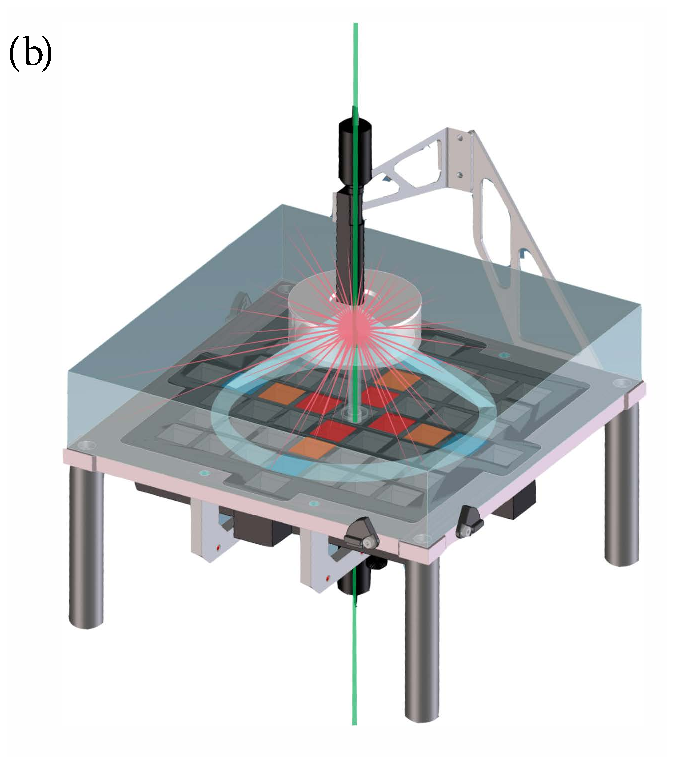
\includegraphics[width=0.45\columnwidth]{chess_timing_setup}
\caption{Detailed schematic view of the CHESS apparatus with dimensions (left), and demonstrating the muon ring-imaging technique (right). The PMT array is designed to hold up to 53 PMTs; the dozen slots occupied for this study are color coded by radius: red and orange for those hit primarily by scintillation photons, and blue for those in the expected Cherenkov ring for LAB and {\labppo}. Due to the lower refractive index, the ring from a water and WbLS targets are detected in the middle (orange) PMTs.}
\label{fig:timing-setup}
\end{figure}

\subsection{Target Vessel}
The target vessel for CHESS is a cylinder 5~cm in radius and 3~cm in height, constructed from ultraviolet-transmitting (UVT) acrylic. 
Three flat faces on the outer surface of the cylinder, each a 3-cm width square, provide surfaces for attaching a radioactive button source or optical coupling of a PMT to act as a trigger for the detector. 
A lid made of the same UVT acrylic encloses the target material in an air-tight environment using an FFKM o-ring~\cite{cog-oring} known to be chemically stable to both {\labppo} and WbLS. 
Each liquid deployed in CHESS uses a separate target to avoid contamination of the target materials.

\subsection{PMT Array}
\label{pmtarray}

One dozen Hamamatsu H11934-200 PMTs~\cite{h11934} were deployed in a cross shape beneath the target.
This geometry providing three radial groups of four PMTs each, and takes advantage of the rotational symmetry of the expected event topology. 
This particular model of PMT was chosen due to its very high quantum efficiency (QE) peaked at $42\%$ (\Cref{fig:optics}) and excellent transit time spread (TTS) of 300~ps (FWHM).

The PMTs are held in a $7 \times 7$ grid, with four additional slots on each side, as shown in~\Cref{fig:timing-setup}. 
The holder was 3D printed from black ABS plastic.
This grid allows for future expansion of CHESS with the purchase and deployment of additional PMTs in the unfilled slots.

\subsection{Cosmic Muon Tags}

Two custom-made cylindrical scintillator tags are positioned above and below the target vessel (\Cref{fig:timing-setup}) in order to tag vertical cosmic muons.  
An aluminum arm maintains the alignment of the upper cosmic muon tag while providing easy access to the target vessel.
The bottom cosmic muon tag is fixed in the center slot of the PMT array. 
Each tag consists of a cylindrical 1-cm diameter Hamamatsu PMT~\cite{h3164} optically coupled to a 1-cm diameter 5-cm tall cylinder of EJ-200 plastic scintillator~\cite{ej200}.
The scintillator is coated with white paint to reflect light into the tag PMT, and then coated with matte black paint (except for the end that is coupled to the PMT) to shield the remainder of the setup from light contamination. 

The small size of the tags results in a low angular acceptance (6$^{\circ}$ from vertical), ensuring a population of events with known orientation and thus a known expectation for the position of the Cherenkov ring.  
Given the typical muon flux at the Earth surface ($1~\mbox{cm}^{-2}\mbox{min}^{-1}$) and the angular acceptance of the tags, an event rate of $\sim4~\mu / \mbox{day}$ is predicted.
This results in datasets that are months long.

\subsection{Optical Propagation}

Cherenkov light from the vertically-going muons is emitted at approximately 45$^{\circ}$from the muon track.
This unfortunately means that an acrylic-air boundary perpendicular to the track would totally internally reflect the Cherenkov photons away from the PMTs.
To resolve this, a large UVT acrylic block (30~cm $\times$ 30~cm $\times$ 6.5~cm) referred to as the optical propagation medium was fabricated to direct photons down towards the PMTs.
The target vessel is optically coupled to the top of this propagation medium, which itself is optically coupled to the PMTs.
This ensures maximal light collection efficiency.
To prevent the vertically-going muons from creating Cherenkov light in this propagation medium, a 1-cm vertical hole was added for the muons to travel through.
Throughout the setup, EJ-550 optical grease~\cite{ej550} is used for optical coupling of components. 

\subsection{Veto Panels}\label{s:veto}

CHESS is positioned within a volume guarded by four scintillator panels (50~cm $\times$ 100~cm $\times$ 5.3~cm), as shown in \Cref{f:veto}, fabricated from EJ-200 plastic scintillator~\cite{ej200} (two on the floor and two on the sides in a corner distribution) providing effective $4\pi$ coverage. 
Each panel is instrumented with a PMT~\cite{9102ksb} which is read out for each event and used for an offline veto. The scintillator panels are used to veto cosmic events during calibration source deployment, and to reject cosmic shower events and coincidence of multiple cosmic muons in the ring-imaging analysis. 

\begin{figure}
\centering
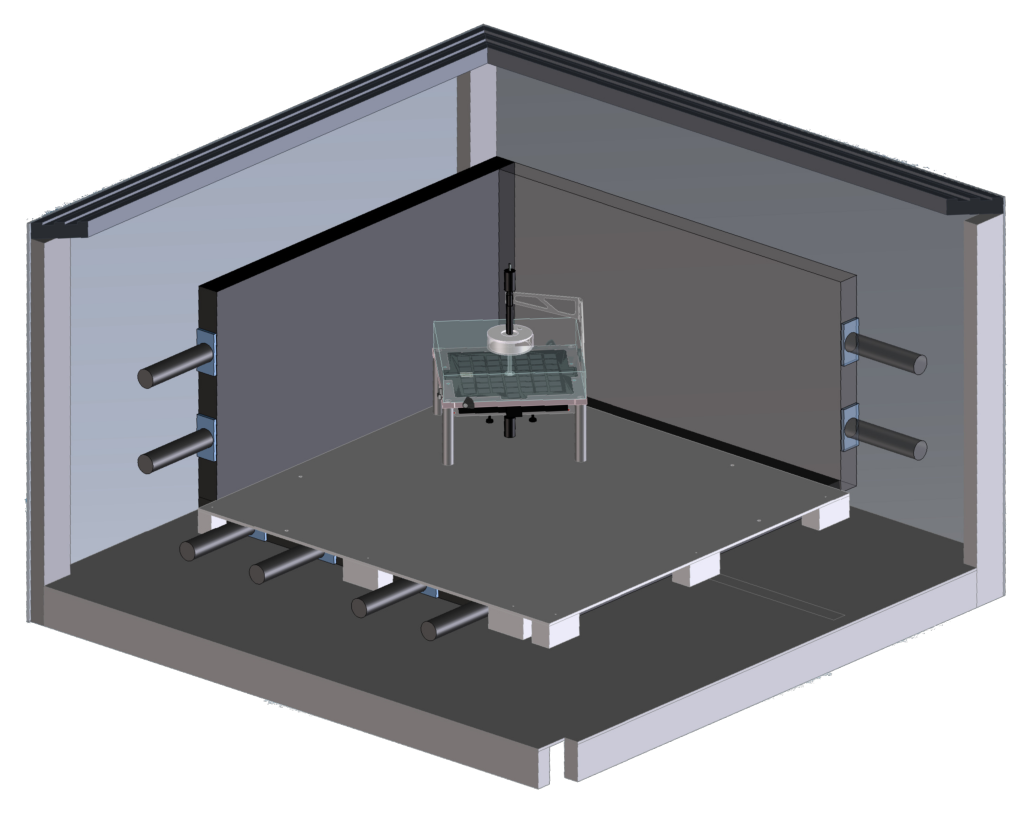
\includegraphics[width=0.7\columnwidth]{veto_panels2}
\caption{Layout of veto panels around the CHESS apparatus. }
\label{f:veto}
\end{figure}


\section{Data Acquisition \label{sec:daq}}

A schematic diagram of the data acquisition (DAQ) hardware is shown in \Cref{fig:daq}  (high voltage omitted) and described in detail in the following sections. 
The DAQ software~\cite{wblsdaq} utilizes the CAEN VME library~\cite{caen-vme} to configure and read out the digitizers and high voltage supplies, and outputs HDF5~\cite{hdf5} formatted files containing raw digitized data and metadata for each triggered event.

\begin{figure}
\centering
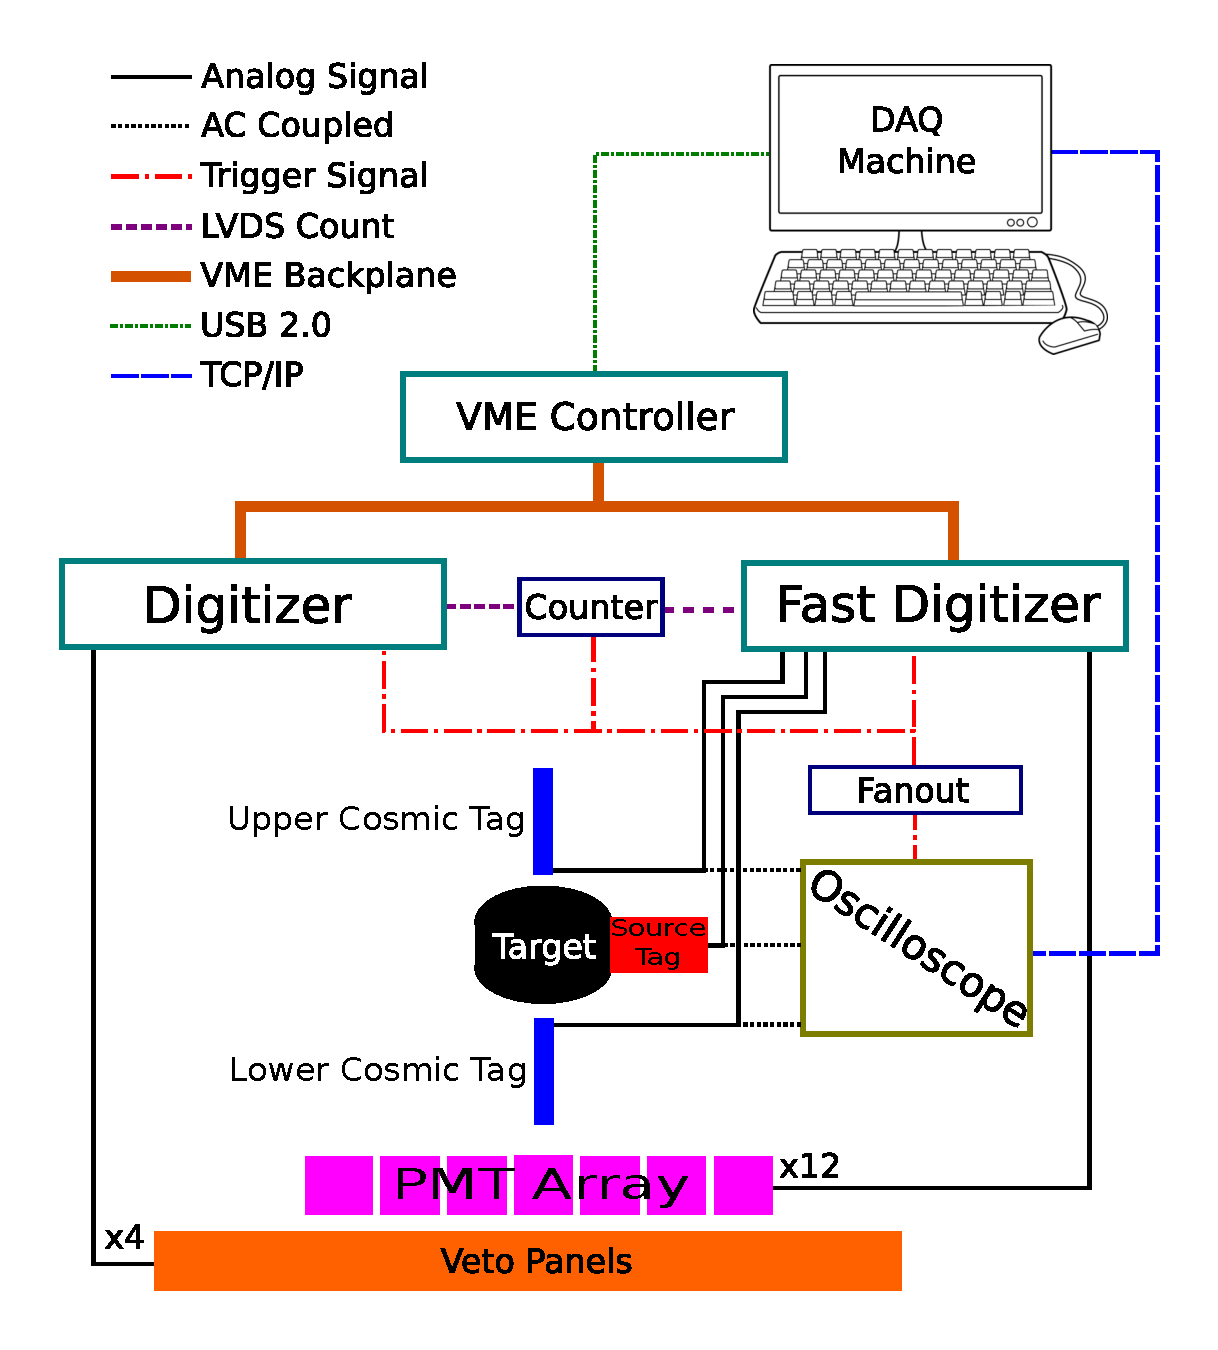
\includegraphics[width=0.7\columnwidth]{daq}
\caption{A schematic diagram of how the DAQ and hardware are connected together with signal and data paths labeled. Omitted are the high voltage supplies, which are connected to the VME backplane, and all PMTs.}
\label{fig:daq}
\end{figure}


\subsection{Readout Electronics and High Voltage}
Three six-channel high-voltage power supplies (CAEN V6533~\cite{v6533}) power the PMTs. 
The PMT output signals are connected to two CAEN digitizers: a high-precision V1730~\cite{v1730} digitizes the veto panels and source tag PMT signals, while a fast V1742~\cite{v1742} based on the DRS4~\cite{drs4} chip digitizes the PMT array and cosmic tag signals.  
The hardware is housed in a VME crate, and a CAEN V1718~\cite{v1718} VME to USB bridge is used for communications.  

The V1742 card is capable of sub-$100$~ps resolution, which exceeds the TTS of the PMT array and is therefore not a limiting factor in the time precision.  
However, on-board buffer size limits the acquisition to a maximum of 1024 samples or 200~ns. 
This shallow buffer necessitated a low-latency triggering scheme in order to contain the pertinent data in the available event window. 
The V1730 digitizer has no dead time between acquisitions, however, the V1742 introduces dead time on the order of 100~$\mu$s.  
A more significant deadtime of 30~ms is introduced by the oscilloscope-based trigger system described in the next section.
This is neither a limitation for measurements with cosmic particles, where the trigger rate is approximately $0.2$~Hz, nor for measurements with radioactive source data where the trigger rate is approximately $30$~Hz.  

\subsection{Trigger System}
\label{sec:triggering}

A LeCroy 606Zi~\cite{lecroy606zi} oscilloscope is used to produce low-latency trigger signals for the setup with programmable coincidence logic. 
Depending on the operating mode one of the following three trigger configurations are used:
\begin{description}
\item [\textrm{\textit{Bottom-only Trigger}}] A threshold condition is applied to the lower cosmic tag only. 
This is the normal operating mode for cosmic data, with the coincidence requirement applied offline.  
A rate of 4 muons/day is expected after the coincidence trigger.
\item [\textrm{\textit{Or Trigger}}] A threshold condition is applied to both of the cosmic tags, and the logical OR of the two is allowed to generate a trigger. 
This mode is used to acquire unbiased charge distributions for each cosmic tag simultaneously.
\item [\textrm{\textit{Source Trigger}}] A threshold condition is applied to the source tag. 
This is the configuration used during radioactive source deployment.
\end{description}
The oscilloscope trigger signal is fanned out to the external trigger input on the V1730 and the low-latency trigger inputs on the V1742.
The V1742 consists of four DRS4 analog sampling chips recording eight channels each.
As these four chips operate on independent high-speed sampling clocks, the trigger signal is also digitized by each chip so that fine time offsets between channels on different chips can be reliably calculated offline.  

\section{Calibration}
\label{sec:calibration}

The setup is calibrated using a $^{90}$Sr beta source in combination with a water-filled target, an LED deployed in the dark box, and a control sample of cosmic muons passing through the acrylic propagation medium. 
For source data, the veto panels are used to reject all cosmic muon events. 
Beta decay, muon ionization, and Cherenkov emission are well understood processes that help to calibrate the optical aspects of the detector. 
The following sections present the calibration scheme.

\subsection{PMT Gain}
\label{pmt-gain}
PMT gains depend on the supplied voltage, which is held constant in CHESS, and also vary between PMTs, depending on the particulars of individual manufacture.
The total charge collected by a PMT from a single PE (SPE) can be modeled as a Gaussian, so measuring the charge collected from single PEs allows one to determine the mean and width of this distribution. 
These parameters are typically measured for each PMT in a detector by using a dim light source known to have fewer than one detected photon per PMT on average.
The $^{90}$Sr beta source attached to the water target provides such a dim source.
A small PMT optically coupled to the target is used to trigger the acquisition, while SPE charge distributions are built for each PMT.

This SPE charge distribution can be sampled multiple times to produce the charge of a multi-photon event.
The charge distribution for one of the array PMTs is shown in \Cref{fig:spe_data}, where a clear SPE distribution is seen. 
Also visible in that figure is a noticeable population of multi PE events, which may be due to byproducts of muon cosmic events crossing the propagation medium, or other intrinsic radioactivity near the detector. 
Muons themselves are easily vetoed using the veto panels surrounding the setup, but high energy electrons and gammas produced by these muons are more difficult to veto, and could cause these tails in the charge distribution. 

A Gaussian fit is used to model the SPE charge distributions. 
To precisely extract the SPE parameters, the noise distribution (events with no charge) and the high charge tails of the data must be taken into account.
A Gaussian is included to model the noise, while additional Gaussians are included to account for multi-PE events. 
The parameters for this noise Gaussian and the normalization of the multi-PE Gaussians are treated as nuisance parameters in the fits.
The means of the multi-PE Gaussians are constrained to be integer multiples, $N$ for the $N$th PE, of the SPE mean, with the widths being $\sqrt{N}$ times the width of the SPE Gaussian.
This results in a fit with 7 parameters: SPE mean and width; noise mean, width, and integral; multi-PE normalization for 2 and 3 PEs.
\Cref{fig:spe_data} shows a sample fit.
Finally, the SPE width is corrected by subtracting in quadrature the width of the noise to arrive at the true width of the SPE charge distribution.

The stability of the PMT gains was checked by taking a second set of water calibration data after data taking was complete.  
The gains for all PMTs in the array were observed to be very stable within measured uncertainties.

\begin{figure}
\centering
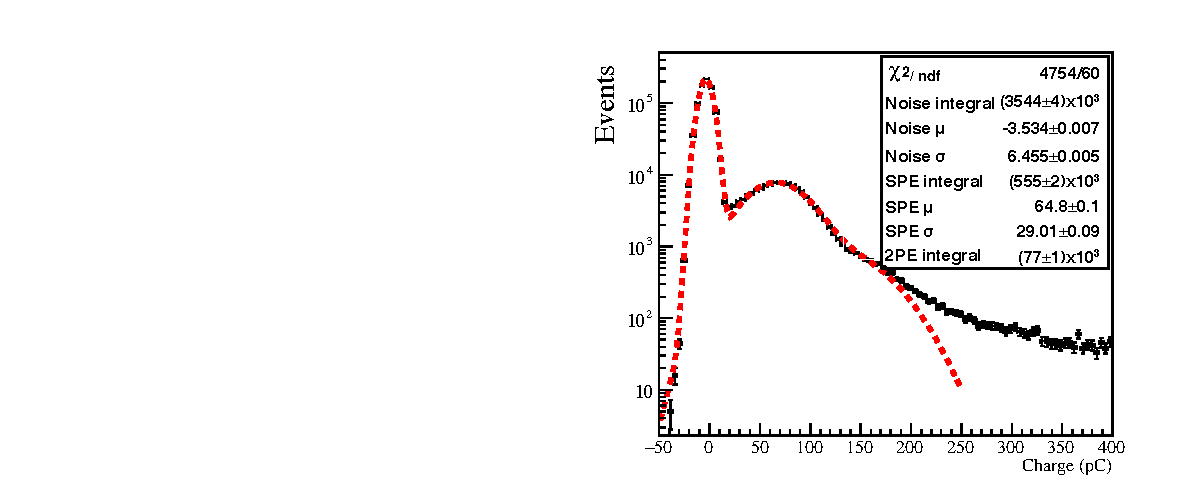
\includegraphics[width=0.7\columnwidth]{spe_ring}
\caption{SPE charge distribution for a single PMT. Data is shown as black points with error bars, and the red dashed line is the result of the fit used to extract the shape of the SPE distribution. }
\label{fig:spe_data}
\end{figure}


\subsection{PMT Pulse Shapes}
\label{sec:pmtpulses}
The characteristic SPE pulse shapes need to be well modeled in order to accurately reproduce the PMT time response in simulation. 
Events with an integrated charge from $-\frac{\sigma}{2}$ to $+\sigma$ about the mean of the SPE charge were extracted from the SPE calibration data for each PMT independently. 
The smaller bound on the negative range was introduced to avoid including noise events. 
These pulses were then normalized to unit area and a constant fraction threshold was applied to determine a common point of reference between all pulses from a single PMT.  
This threshold was used to align pulses on a per-PMT basis, and a mean value along with upper and lower RMS values were calculated for the normalized voltage in 100-ps time bins.
The result is shown for one PMT in the top panel of \Cref{fig:spe-pulse-shape}. 
The uncertainty in the pulse region is consistent with the noise of the ADCs; this was true for all PMTs. 
The extracted mean PMT pulse shapes are shown for all 12 array PMTs in the middle panel of \Cref{fig:spe-pulse-shape}. 
The PMT-to-PMT variation in pulse shape is attributed to small variations in voltage dividers, signal coupling circuits, and individual PMT construction. 
A log normal of the form 
\begin{eqnarray}
\frac{1}{\sigma \sqrt{2\pi}}\exp{\left[\frac{-\left(\log[t-t_0]-\mu\right)^2}{2\sigma^2}\right]}
\end{eqnarray}
was fit to the average pulse shape across all 12 PMTs (lower panel of \Cref{fig:spe-pulse-shape}) and the resulting fit parameters were used in the simulation to model PMT pulse shapes.

\begin{figure}
\centering
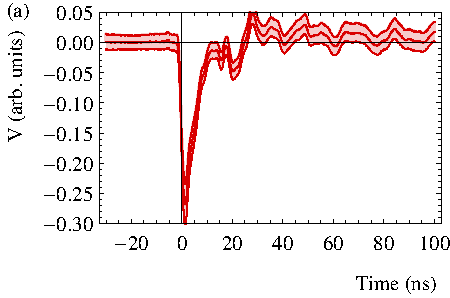
\includegraphics[width=0.5\columnwidth]{pulse_shape_ring1}
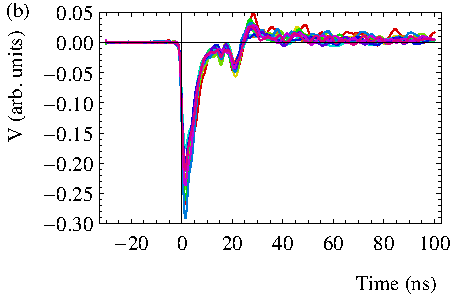
\includegraphics[width=0.5\columnwidth]{pulse_shape_norm_ring}
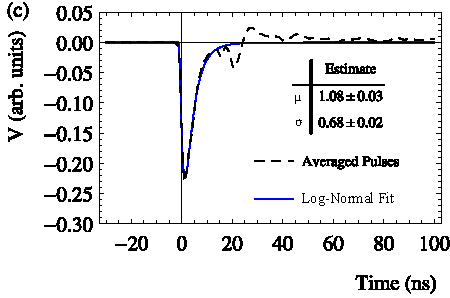
\includegraphics[width=0.5\columnwidth]{pulse_shape_lognorm_fit}
\caption{PMT pulse shape characterization.   
(a) Mean and RMS spread for one PMT, showing excellent stability in the pulse region.  
(b) Averaged pulse shapes for SPE pulses for each individual PMT. 
(c) Log-normal fit to the average pulse shape across all PMTs. 
In all cases the pulses are normalized to unit area, so the voltage is reported in arbitrary units.}
\label{fig:spe-pulse-shape}
\end{figure}


\subsection{Per-Channel Time Delays}\label{s:delay}

The total time delay due to PMT transit times, electronics, and cable lengths is measured for each individual channel and is used to correct hit times from the data. 
Time delays are measured relative to the average across all PMTs in the array. 
Typical relative delays are on the order of hundreds of picoseconds. 
The primary calibration is performed by deploying an LED at the top of the dark box, such that the light path to each PMT is similar.  A full Monte Carlo (MC) simulation of this configuration is run and used to correct the data in order to take into account PMT-to-PMT variations in photon time of flight (ToF) and geometry effects.  
Several datasets are generated by removing and reattaching the LED in order to quantify any uncertainty in the LED position with respect to the simulated one. 
Cosmic muons passing through the propagation medium are used to evaluate systematic uncertainties in the calculation of the time delays, as they provide an abundant source of prompt Cherenkov light. 
Events are selected  by requiring a coincidence between the lower muon tag and the bottom scintillator panel. 
Again, a full MC simulation is used to correct for ToF and geometry effects in the calibration.  

The time distribution for one channel is shown in the upper panel of \Cref{fig:time_delay}, where the offset represents the time delay with respect to the average. 
The measured time delays with uncertainties for each channel from each calibration are shown in the lower panel of \Cref{fig:time_delay}.  
The two datasets show the same trend across the PMT array.  
The MC-corrected LED dataset is used to define the time delays for the final separation analysis.
The difference between the two datasets is taken as a measure of  systematic error in this calibration.  

\begin{figure}
\centering
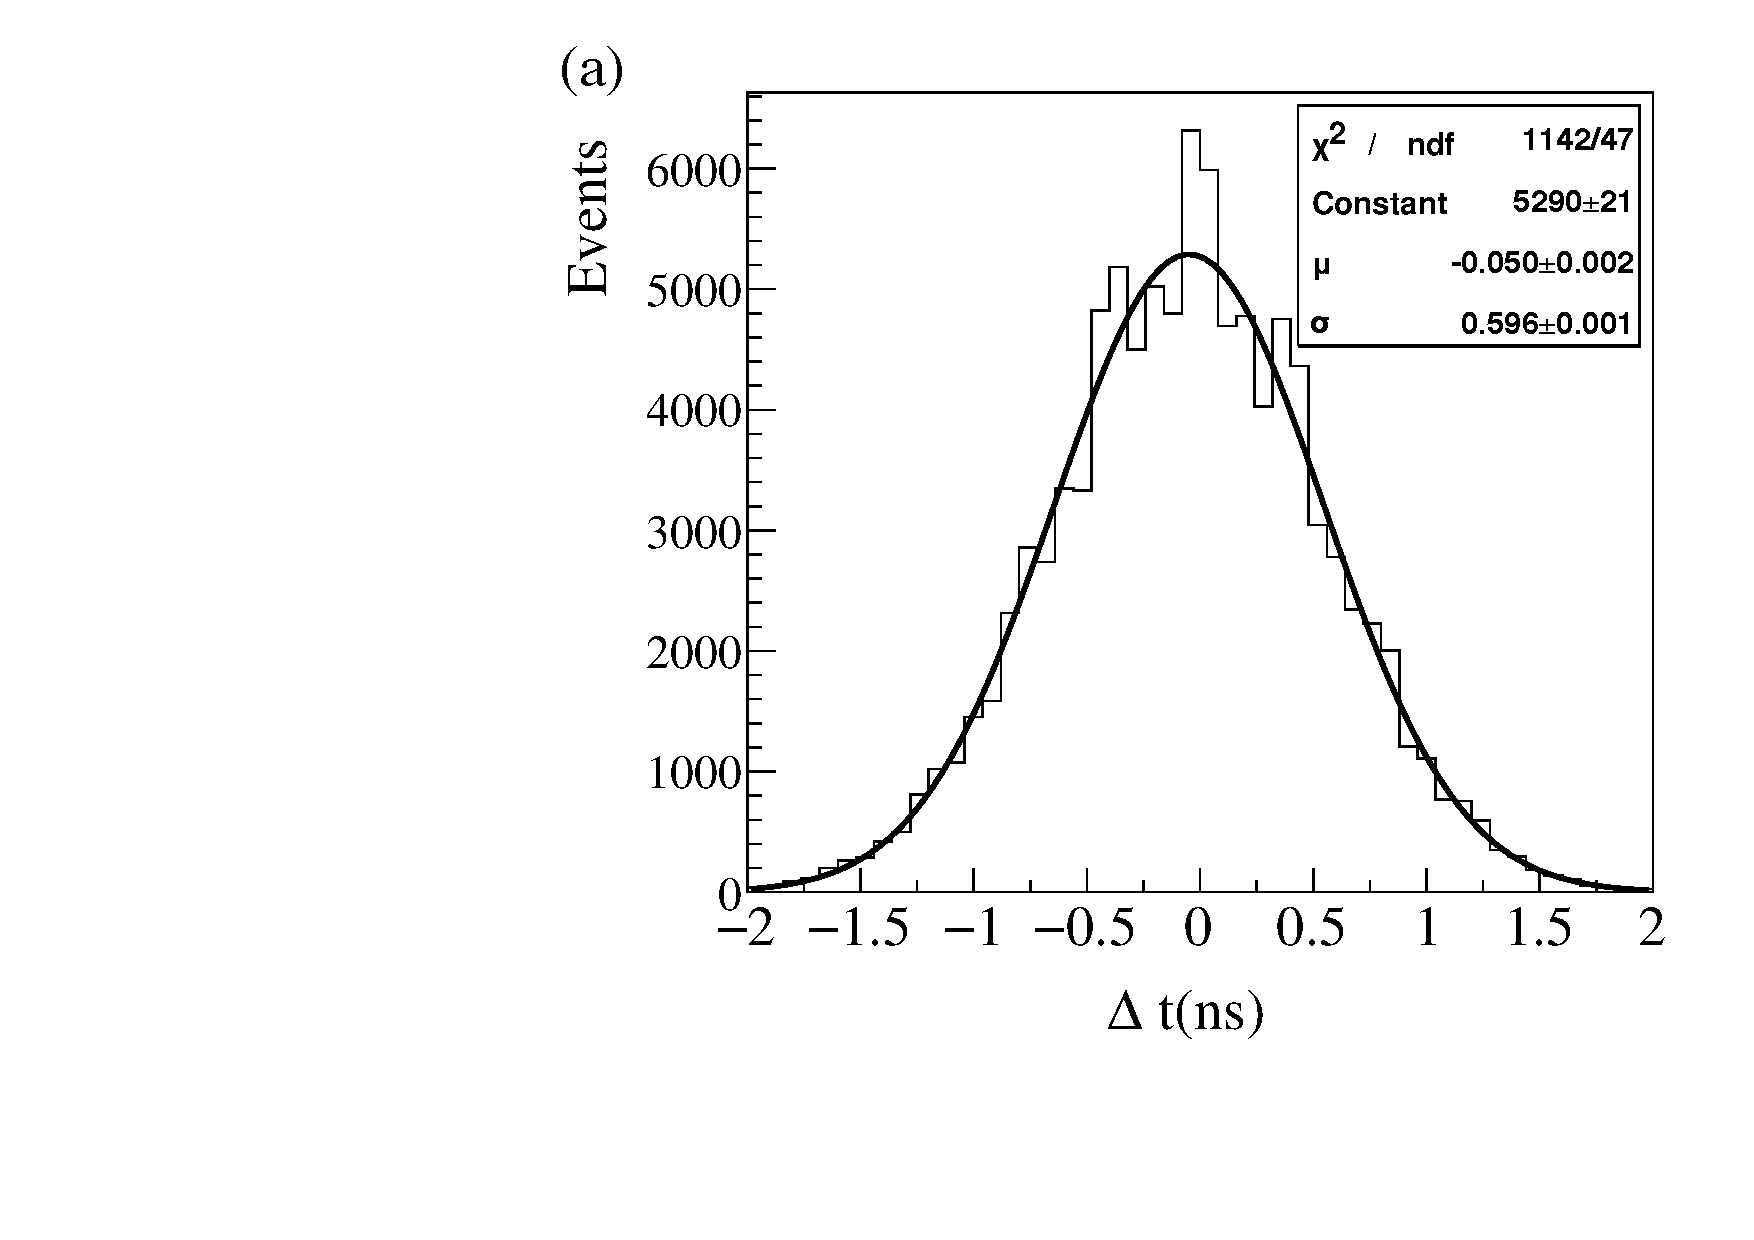
\includegraphics[width=0.6\columnwidth]{time_delays_ledtop_singlepmt}
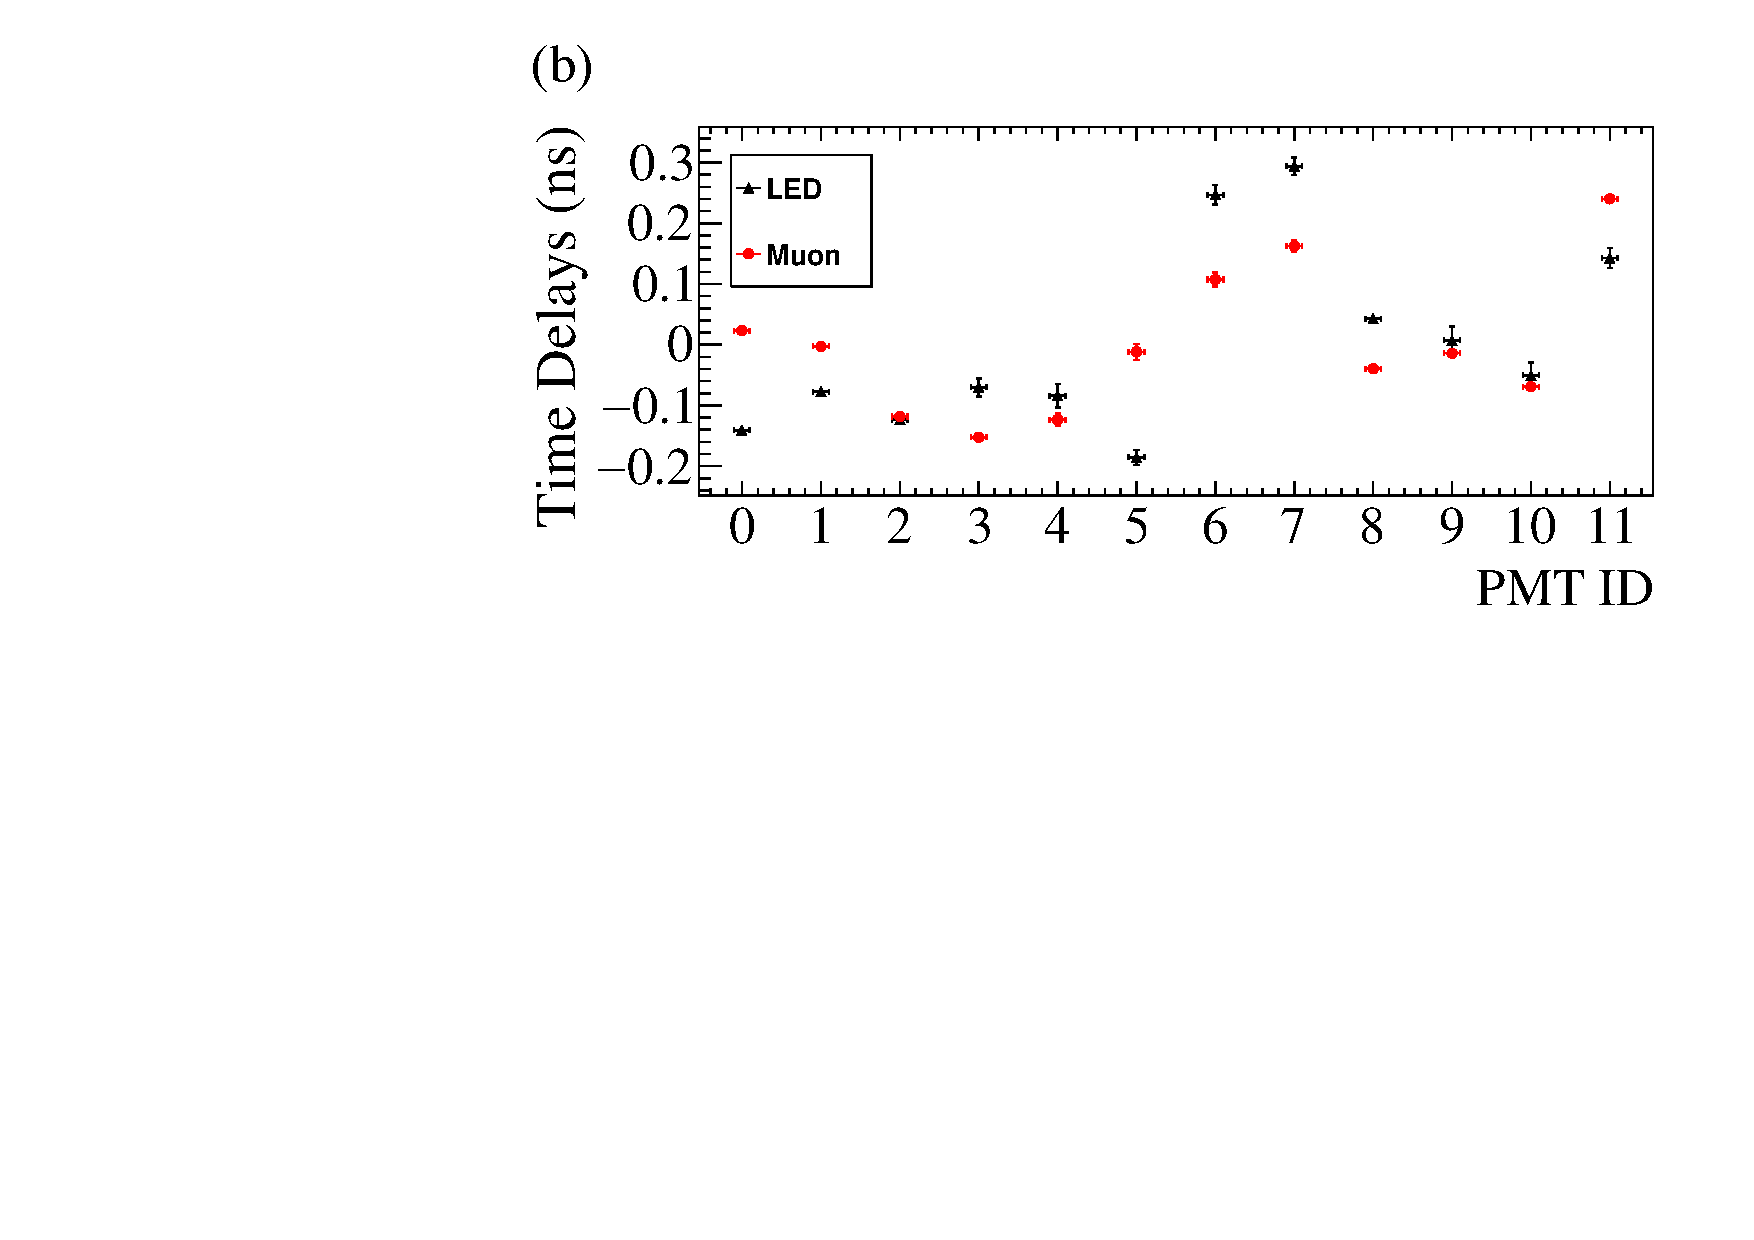
\includegraphics[width=0.6\columnwidth]{time_delays_ledaverage_muon}
\caption{(a) Time distribution for a single channel relative to a reference channel, overlaid with the Gaussian fit used to extract the relative time delay.  (b) Mean and uncertainty on the mean for the per-channel time delays.}
\label{fig:time_delay}
\end{figure}


\section{Monte Carlo Simulation}
\label{sec:simulation}

The entire setup is simulated in the open source program RAT-PAC~\cite{ratpac}, which is closely related to the RAT software used by {\snop}. 
Primary particles are produced and tracked in a complete geometry implemented in GEANT4~\cite{geant4}. 
When Cherenkov and scintillation processes take place, individual photons are tracked from the production point to the PMTs. 
Once the photon reaches the PMT, a custom model decides whether to produce a photoelectron (PE) based on the photon properties and PMT features. 
If any PE are produced in a PMT for an event, a custom DAQ simulation generates a simulated waveform for that PMT to be analyzed with the same algorithms applied to data.
These different stages of simulation are described in the following sections.

\subsection{Cosmic Muon Generator}
\label{sec:primarygen}

Muons and anti-muons are generated at $50\%$ ratio following the semi-empirical modified Gaisser distribution~\cite{gaisser-mod}. 
Generated muons are constrained to pass through the bottom tag volume, as this is the trigger signal for the detector. 
Coincidence constraints between the bottom and top tag are applied in offline analysis.
There exists the possibility that high energy delta rays (electrons produced by muon ionization) may trigger one of the cosmic tags, resulting in false coincidence.
This is reproduced in simulation by including a complete model of the holder material and geometry for both top and bottom tags.

\subsection{Photon Production \label{sec:photon_prod}}

Cherenkov production is simulated by GEANT4 by the standard model implemented in G4Cerenkov. 
The typical Cherenkov emission spectrum is shown in \Cref{fig:optics}.

Scintillation emission is handled by a minimally modified version of the GLG4Scint model~\cite{glg4sim}. 
A charged particle passing through a medium deposits an energy $E$ due to ionization. 
The total number of scintillation photons generated is not expected to behave linearly with $E$ due to quenching effects in the scintillator.
This is taken into account by GLG4Scint by using Birk's law~\cite{birks} which states that the deposited energy after quenching, $E_{q}$, is:
\begin{eqnarray}
\dfrac{dE_{q}}{dx} = \dfrac{dE/dx}{1+ k_BdE/dx},
\label{eq:birk}
\end{eqnarray}
where $k_B$ is Birk's constant, which must be determined for any particular scintillator. 
The total number of  photons produced, $N_{\gamma}$, is directly proportional to $E_{q}$, where the proportionality constant is typically called the light yield of the material. 

Scintillation photons are emitted with some characteristic time profile, $\rho(t)$, typically modeled as an exponential rise and a sum of exponentially decaying terms of various time constants.
This time profile is well described by a double exponential model~\cite{mcguire_palmer}, including both a rise time and a decay time. 
Two further decaying exponentials are included for {\labppo}, based on measurements in~\cite{labppo}. The simulated time profile is:
\begin{eqnarray}
\rho(t) \propto (1 - e^{-t/\tau_r}) \times \sum^3_i A_i e^{-t/\tau_i},
\end{eqnarray}
where $\tau_r$ is the rise time and the parameters $\tau_i$ and $A_i$ are the decay times and their scale factors.
RAT-PAC also supports the use of an arbitrary PDF as the scintillation time profile.
Similarly, scintillation photons follow some wavelength distribution, often called an emission spectrum, for which RAT-PAC accepts an arbitrary PDF.

\textit{Ex-situ} measurements for the scintillation emission spectrum, light yield, and time profile are included in the simulation. 
The procedure for generating scintillation photons draws $N_{\gamma}$ photons randomly from the emission spectrum and time profile of the scintillator under investigation. 
For reference, the spectra for LAB~\cite{lab_emission} and {\labppo}~\cite{snop_private} are shown in \Cref{fig:optics}. 


\subsection{Optical Propagation \label{sec:optics}}

Optical photons are propagated through different media by GEANT4. 
Absorption, refraction and reflection are taken into account according to the optical properties defined for each material. 
The absorption length of the UVT acrylic used in CHESS (\Cref{fig:optics}) was measured with a spectrometer and is included directly in the simulation.  
The refractive indexes for LAB and {\labppo} are considered to be the same and are taken from~\cite{snop_private}.
Photon reemission from wavelength shifting materials are simulated in a similar fashion as the scintillation process. Once a photon is absorbed in a scintillating medium, there is a finite probability that it will be reemitted by again randomly sampling the emission spectrum.

\subsection{PMT Model \label{sec:pmt_model}}

Detailed PMT geometries (glass, photocathode, dynode stack and case) are included in RAT-PAC, as well as a fast photon tracking simulation inside the PMT volume. 
Once an optical photon hits the external boundary of the PMT glass, it is propagated directly from one dielectric interface to another according relevant refractive indices until it is absorbed in the photocathode, absorbed at an interface, or escapes the PMT.
This ignores additional effects considered by GEANT4 during normal photon propagation outside the PMT, resulting in a significant speedup of the simulation.

The QE of the PMTs is taken from Hamamatsu specifications~\cite{h11934} and used by the simulation to determine whether or not to create a PE for an incident photon at a particular wavelength. 
The collection efficiency of generated PE can be simulated per PMT, however these are set to a nominal 90\% for each PMT according to Hamamatsu specifications~\cite{hamamatsu}.  
If the incident photon creates a PE, the total amplified charge and detection time are extracted from Gaussian distributions that have been previously calibrated to take into account the calibrated PMT gain and electronic delays.

The SPE charge distribution is modeled as a Gaussian truncated at zero to exclude negative charge values. 
The mean and width of this distribution are taken from the previously described gain calibration, and \Cref{fig:spe_data} shows that the Gaussian model agrees well with the data.

Each PMT has a characteristic transit time and transit time spread (TTS) that depends strongly on the internal design of the PMT. 
Nominal values for the TTS are taken from the PMT specifications and included in the simulation by assuming the detected time is Gaussian distributed.
The PMT specifications~\cite{h11934} show that the Gaussian TTS model is a very good approximation.

\subsection{DAQ Simulation \label{sec:daq_sim}}

For each event an analog waveform is generated per channel by summing the individual pulses created by each PE.
The SPE waveform shapes determined in calibration are used here, and scaled by the charge detected by each PMT.
The waveform is then digitized via a process that mimics the characteristics of the two models of CAEN digitizers used in the detector. 
High frequency electronics noise is added to these digitized waveforms following a Gaussian distribution centered at zero and with a width of $0.35$~mV and $0.88$~mV for the V1730 and V1742 cards, respectively.
These widths are measured from data by measuring the RMS of force-triggered noise data from the detector.
This allows the simulation to reliably reproduce digitized traces for each PMT for each event.

The trigger process implements the conditions described in \Cref{sec:triggering} and decides whether to create a triggered detector event. 
When an event is created, acquisition windows corresponding to the buffer size of the appropriate digitizer are captured from the simulated waveforms.
These windows are used to determine photon hit times and charge using the same process as applied to data in \Cref{s:analysis}.  
The trigger process then scans the remainder of the digitized waveform to look for additional triggers within the same simulated physics event, in an analogous way to the functioning of the physical DAQ.


\section{Waveform Analysis}\label{s:analysis}

The CHESS detector fully digitizes the PMT signals for each triggered event.
These waveforms must then analyzed to extract individual PMT charges and hit times. 
The acquisition trigger is delayed relative to the signals from the PMTs because the LeCroy oscilloscope takes about 150~ns to issue the trigger signal that is propagated to the digitizers. 
Accounting for this delay, an analysis window of $135$~ns (675 samples) is chosen to start $160$~ns (800 samples) prior to the acquisition trigger. 
A short 25~ns pedestal window prior to the analysis window is used to estimate the voltage baseline for each PMT for each event.
The baseline is subtracted off the analysis window, and the residuals are integrated to determine the total charge detected by each PMT. 
To ensure that this process works reliably, fluctuations of more than $5$~mV peak-to-valley in the pedestal window results in the event being discarded in offline analysis.  
The integrated charge is used to estimate the number of PE by dividing by the mean of the SPE distribution for that PMT as determined in calibrations (\Cref{sec:calibration}).

A discriminator is implemented in the analysis software to determine the hit time of each PMT.
If the waveform crosses a threshold given by $25\%$ of the height of a single PE pulse, a hit time is computed at that crossing.
This threshold is determined per PMT by modeling the PMT pulse shape as a log-normal pulse with parameters extracted from the fit in \Cref{sec:pmtpulses} and requiring integrated charge equivalent to the mean of the SPE distribution measured for each PMT.
This threshold is well clear of the electronics noise, as can be seen in \Cref{fig:spe-pulse-shape}. 

Linear interpolation between digitized samples is used to maximize the time precision. 
Finally, these hit times are corrected by the expected time of flight (ToF) between the center of the target vessel and each PMT in order to find the creation time of each detected photon, which can be compared between PMTs regardless of PMT position.


\section{Cosmic Muon Event Selection}\label{s:event}

A deionized water target was used to develop event selection criteria in order to select clean Cherenkov ring events.
Simply requiring a coincidence between the muon tags is not sufficient due to instrumental backgrounds and events where the muon did not cleanly travel through the setup.
Two notable backgrounds are non-vertical muons that trigger both tags and also travel through the acrylic block, and production of energetic electrons along the muon track.
In both cases, light is produced in regions other than the target, which interferes with the ability to classify detected photons based on the ring geometry of Cherenkov light.

The goal here is to develop selection criteria on water that can be applied to any other target.
These criteria are then used to select events that should contain Cherenkov rings in LS datasets.
The criteria were defined by classifying all events in the water dataset according to the clarity of a visible Cherenkov ring, and then adjusting relevant cut values to maximize acceptance of good ring candidates and minimize contamination by non-Cherenkov-like events.
The methodology is described in the following sections.

\subsection{Event Classification}\label{s:class}
Events in the pure water dataset were hand scanned in order to understand the different types of event topology and their sources.
A classification scheme was developed to sort them according to how well they matched the expected Cherenkov ring geometry, for the purposes of defining a quantitative set of event-selection criteria. 

PMTs with an integrated charge greater than one third of the SPE charge for that PMT were counted as hit.  
Hits were grouped according to the radius of the hit PMT.  
The cross-shape PMT deployment results in three radial groupings: the \textit{ inner}, \textit{ middle} and \textit{ outer} PMTs.  
The CHESS apparatus was designed such that the Cherenkov ring falls on the middle ring for a water target, and the outer ring for a pure LS target.  
The total number of hit PMTs within each grouping, 
NHit$_{inner}$, NHit$_{middle}$, and NHit$_{outer}$, was determined by summing hits across all PMTs within that group. 
A perfect Cherenkov ring in water is expected to have NHit$_{middle} = 4$ while NHit$_{inner} = \mathrm{ NHit}_{outer} = 0$. 
``Ring'' events were selected with the criteria NHit$_{middle} - \mathrm{ NHit}_{inner} - \mathrm{ NHit}_{outer} > 2$ to allow either one expected PMT to be missed or one additional PMT to be hit (but not both) to allow for minor noise contamination and increased acceptance.

``Background'' events were sorted into categories according to  event topology, in order to understand the primary sources of background.  
These included instrumental events, which had no clear ring, so-called ``follower'' events, in which a secondary particle generated Cherenkov light in the propagation medium, causing unusually high charge on the inner PMTs, and events in which a cosmic muon shower lit up the majority of PMTs within the array.

\subsection{Cut Development}\label{s:cut}
An initial selection of vertical-going cosmic muon events was achieved by requiring a triple coincidence between the cosmic muon tags and the scintillator panel directly below the detector.  

Rejection of events containing either multiple muons or secondary particles was achieved by requiring the charge on all veto panels except the panel directly below the setup (which is always hit for vertical muons) to be consistent with zero.  

The threshold values applied to the charge seen on the cosmic tags ($Q_U$ and $Q_L$ for the upper and lower tag, respectively), and for each of the muon panels ($Q_{V1}$ --- $Q_{V4}$) were selected by optimizing acceptance of ``ring'' events and rejection of ``background'' events.  
The data before and after application of these cuts is shown in \Cref{fig:event-selection-cuts}.

\begin{figure*}
\centering
\begin{tabular}{cc}
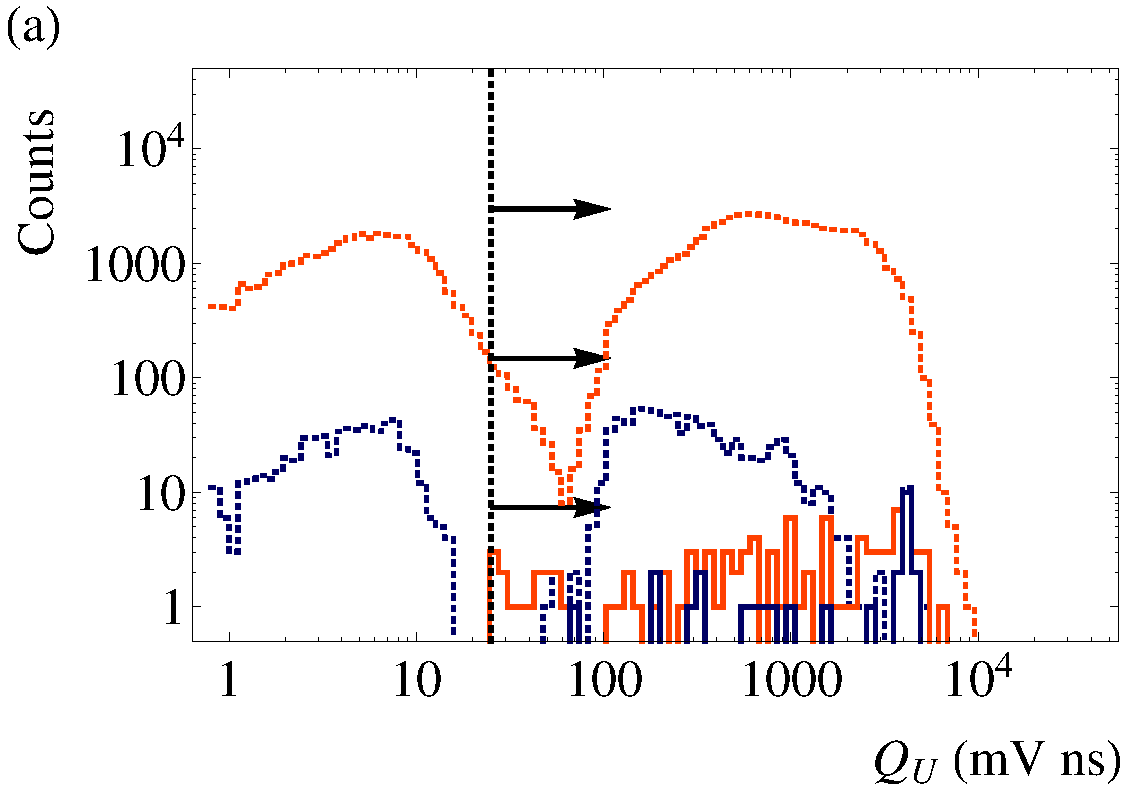
\includegraphics[scale=0.4]{water_nimpaper_cuts_gbsimpleveto_top_tag} &
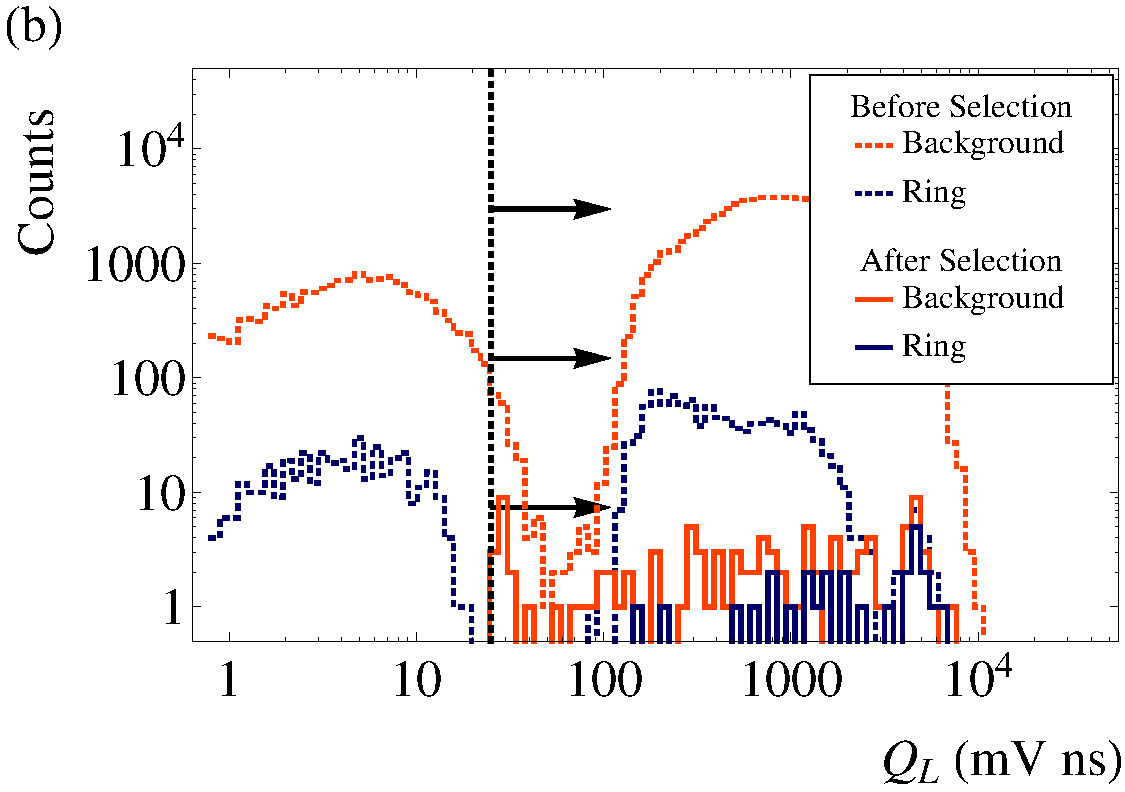
\includegraphics[scale=0.4]{water_nimpaper_cuts_gbsimpleveto_bot_tag} \\
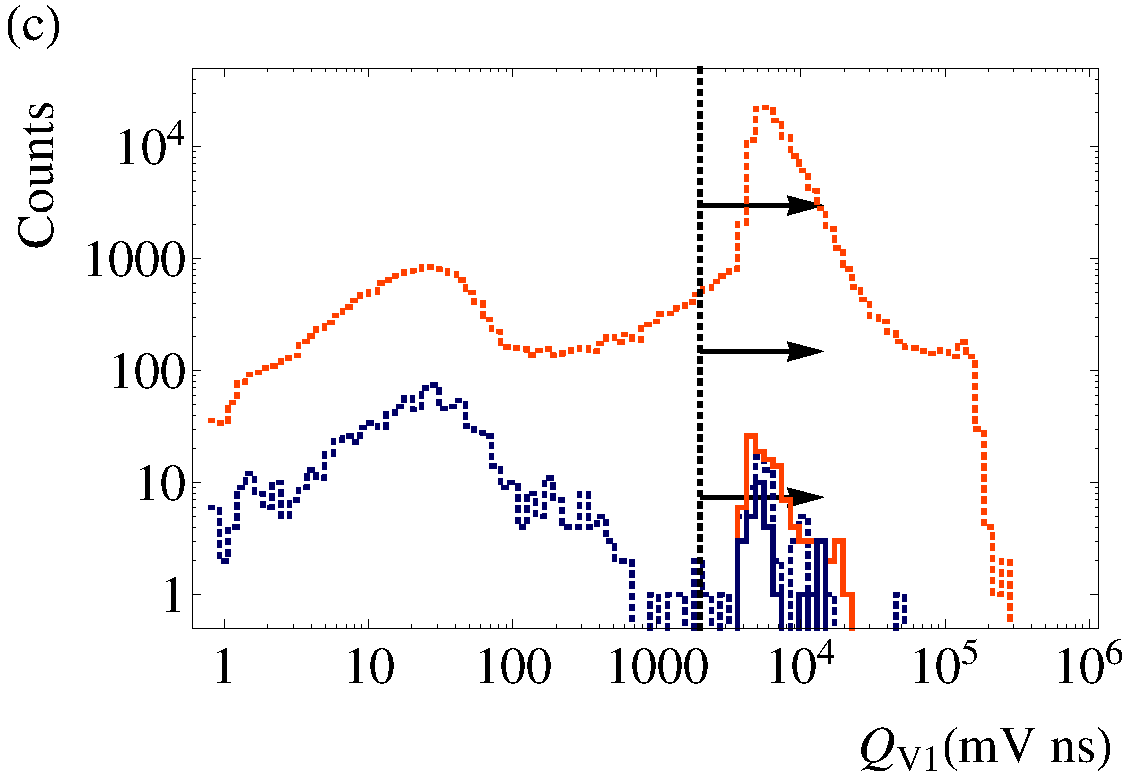
\includegraphics[scale=0.4]{water_nimpaper_cuts_gbsimpleveto_veto1} &
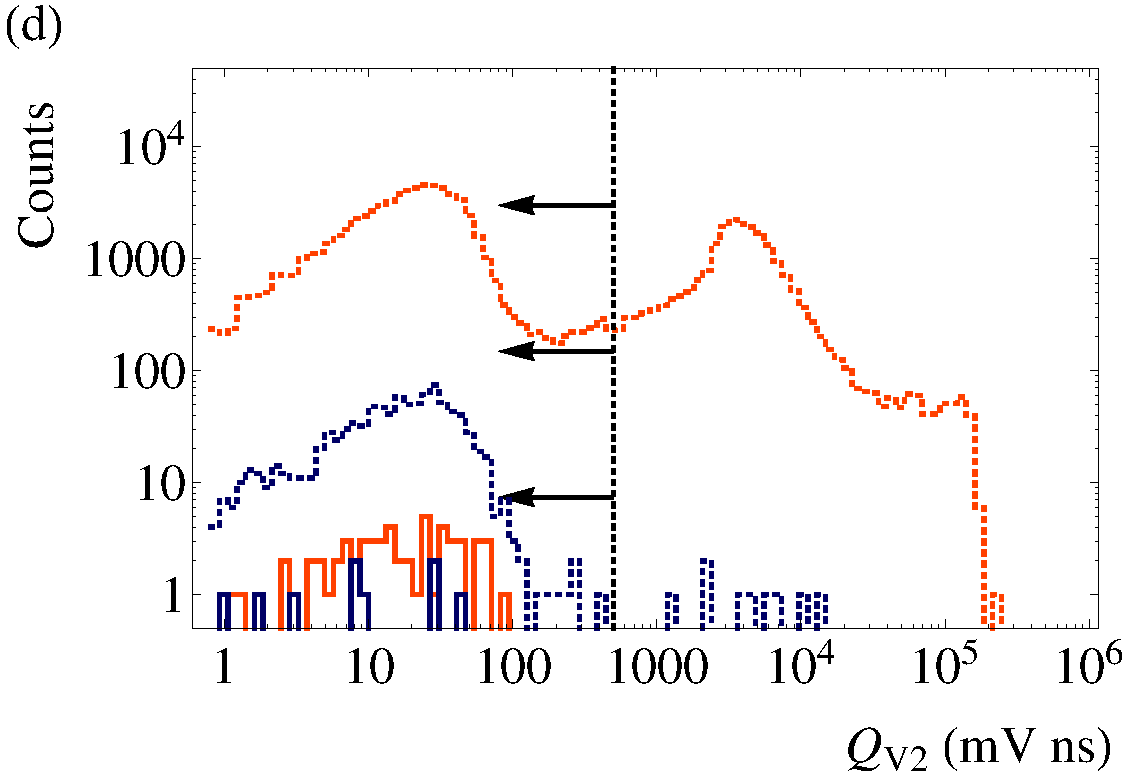
\includegraphics[scale=0.4]{water_nimpaper_cuts_gbsimpleveto_veto2} \\
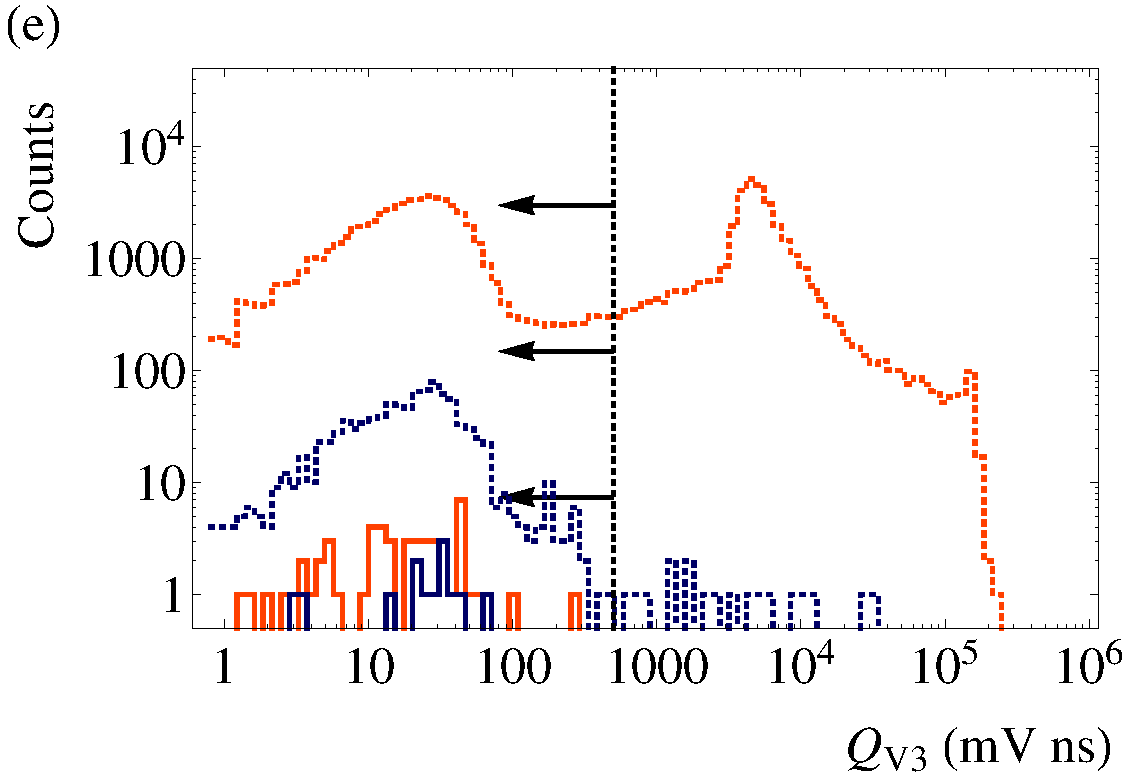
\includegraphics[scale=0.4]{water_nimpaper_cuts_gbsimpleveto_veto3} &
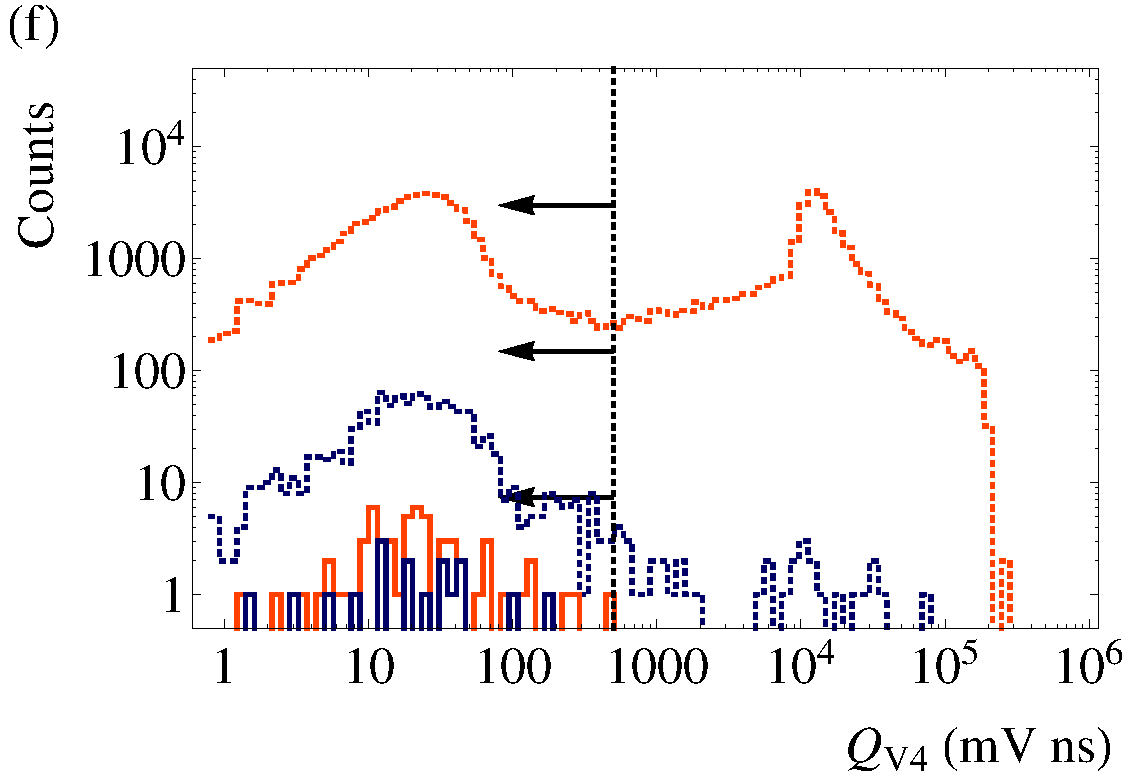
\includegraphics[scale=0.4]{water_nimpaper_cuts_gbsimpleveto_veto4} \\
\end{tabular}
\caption{(Top to bottom, left to right) Charge distribution of events on the upper and lower cosmic tags ($Q_U$ and $Q_L$) and the four muon panels ($Q_{V1}$ --- $Q_{V4}$).  Panel 1 is located directly below the CHESS apparatus.  Events are separated into ring (blue, lower line) and background (red, upper line) according to the criterion in \Cref{s:class}.  Vertical black dashed lines show the cut values in each case with arrows indicating the acceptance region.  Distributions are shown before (dashed) and after (solid) application of cuts on these 6 parameters.}
\label{fig:event-selection-cuts}
\end{figure*}

Cuts were also applied to remove so-called ``follower'' events, in which muons or muon followers generated Cherenkov light in the acrylic propagation medium.
MC indicates that two processes are responsible for a majority of these events: 
\begin{itemize}
\item \emph{Electron contamination:} The cosmic muon triggered the acquisition, but a secondary particle passed through the propagation medium.
\item \emph{Muon contamination:} The secondary particle triggered the lower muon tag and the muon itself passed through the propagation medium.  
\end{itemize}
The secondary particles do not always make it to the veto panels and therefore cannot be vetoed directly, thus the only information available for rejecting these events is the PMT array.  
Unfortunately, this means that this selection criteria is not target independent, however, the effect can be studied in MC to develop a cut on the data.
Clean cosmic muon events are expected to produce hits only on the middle PMTs (for a water target, or outer PMTs for LS).
In both cases of follower events, the majority of Cherenkov light generated in the propagation medium was observed to fall primarily on the innermost PMTs within the array.  
This was confirmed by MC simulations of each event type, which demonstrated that muon followers do produce events with this topology.   
Simulations of these events shown in \Cref{f:clipMC} show a clear tail in the PE distribution observed on the inner PMT group for both water and {\labppo} targets.
These events typically create between 30 and 400 PEs in the innermost PMTs, which is significantly higher than the expected number of PE of a clean event, allowing them to be identified and removed from the data.

\begin{figure}
\centering
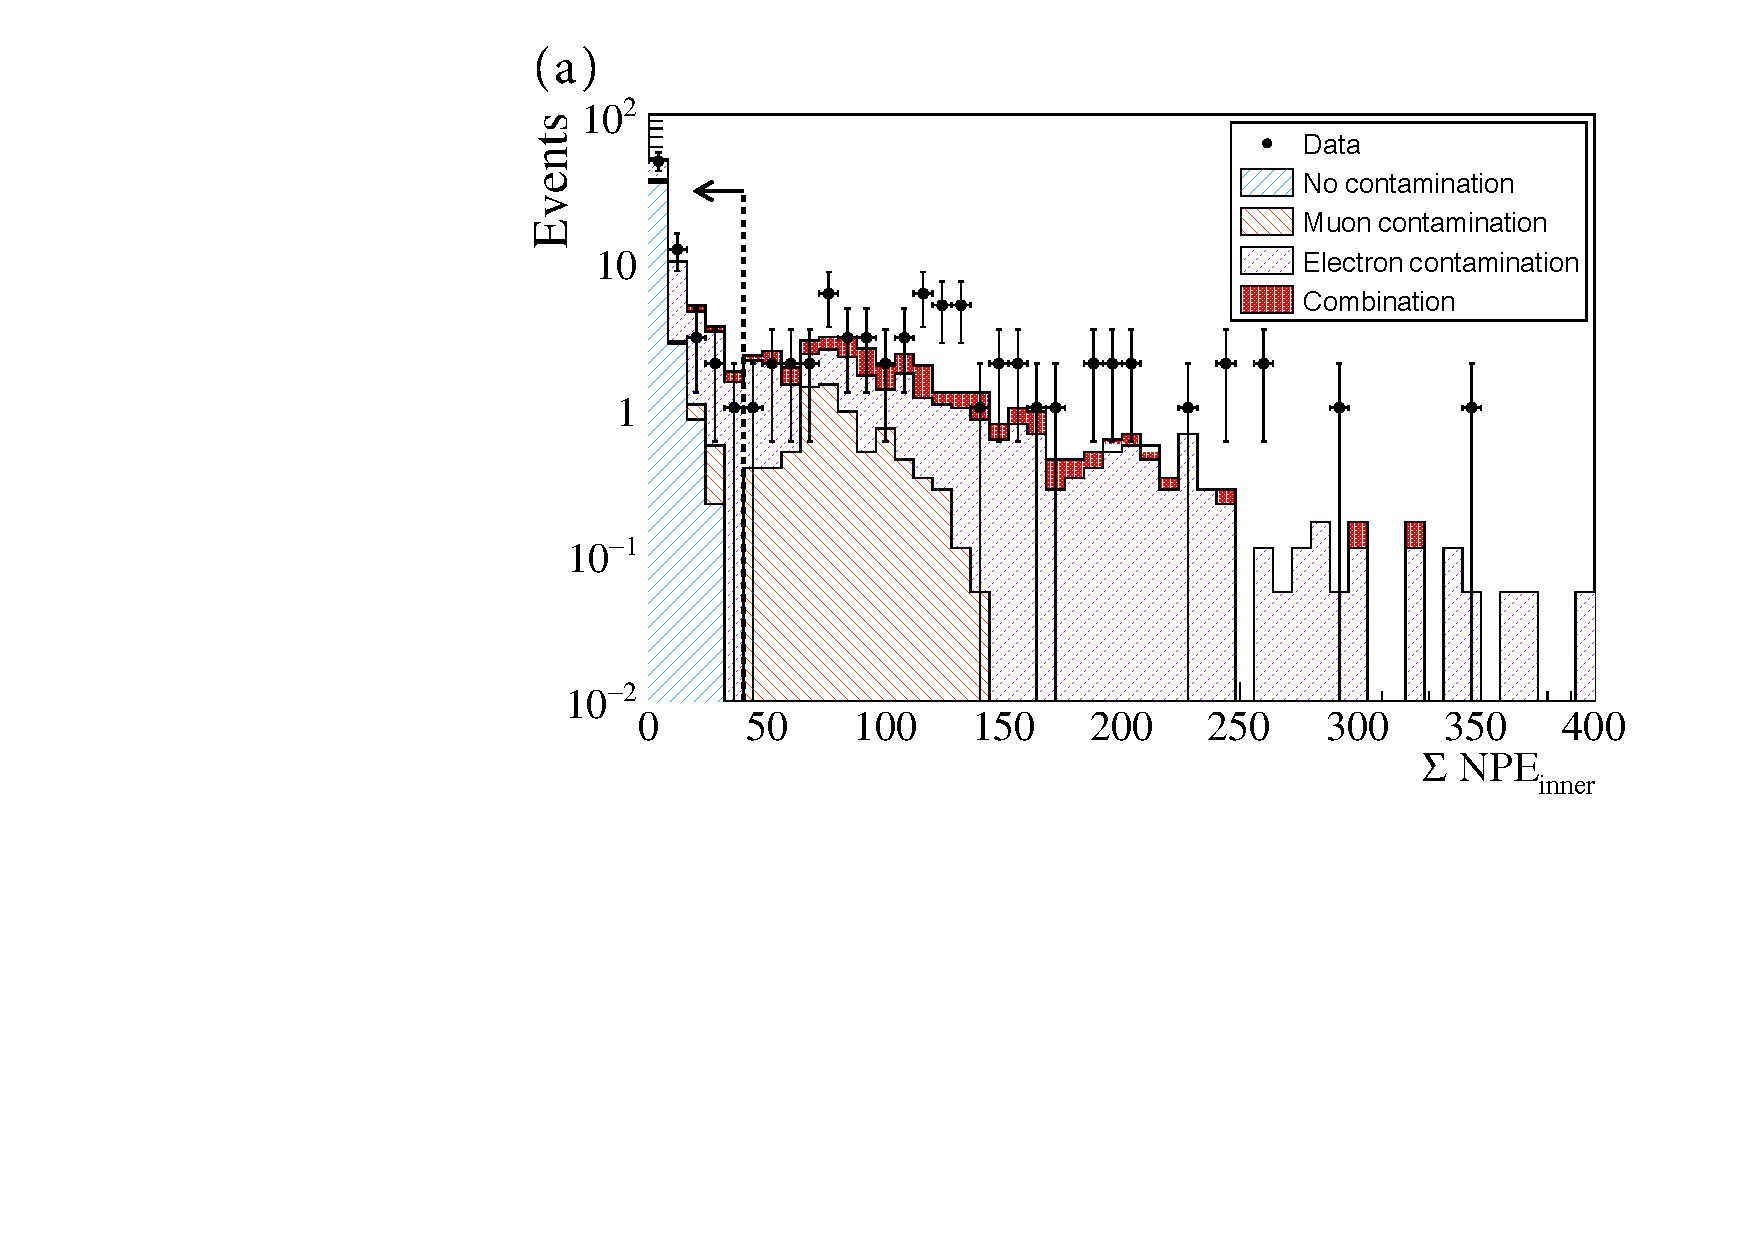
\includegraphics[width=0.6\columnwidth]{cosmic_water_clipping}
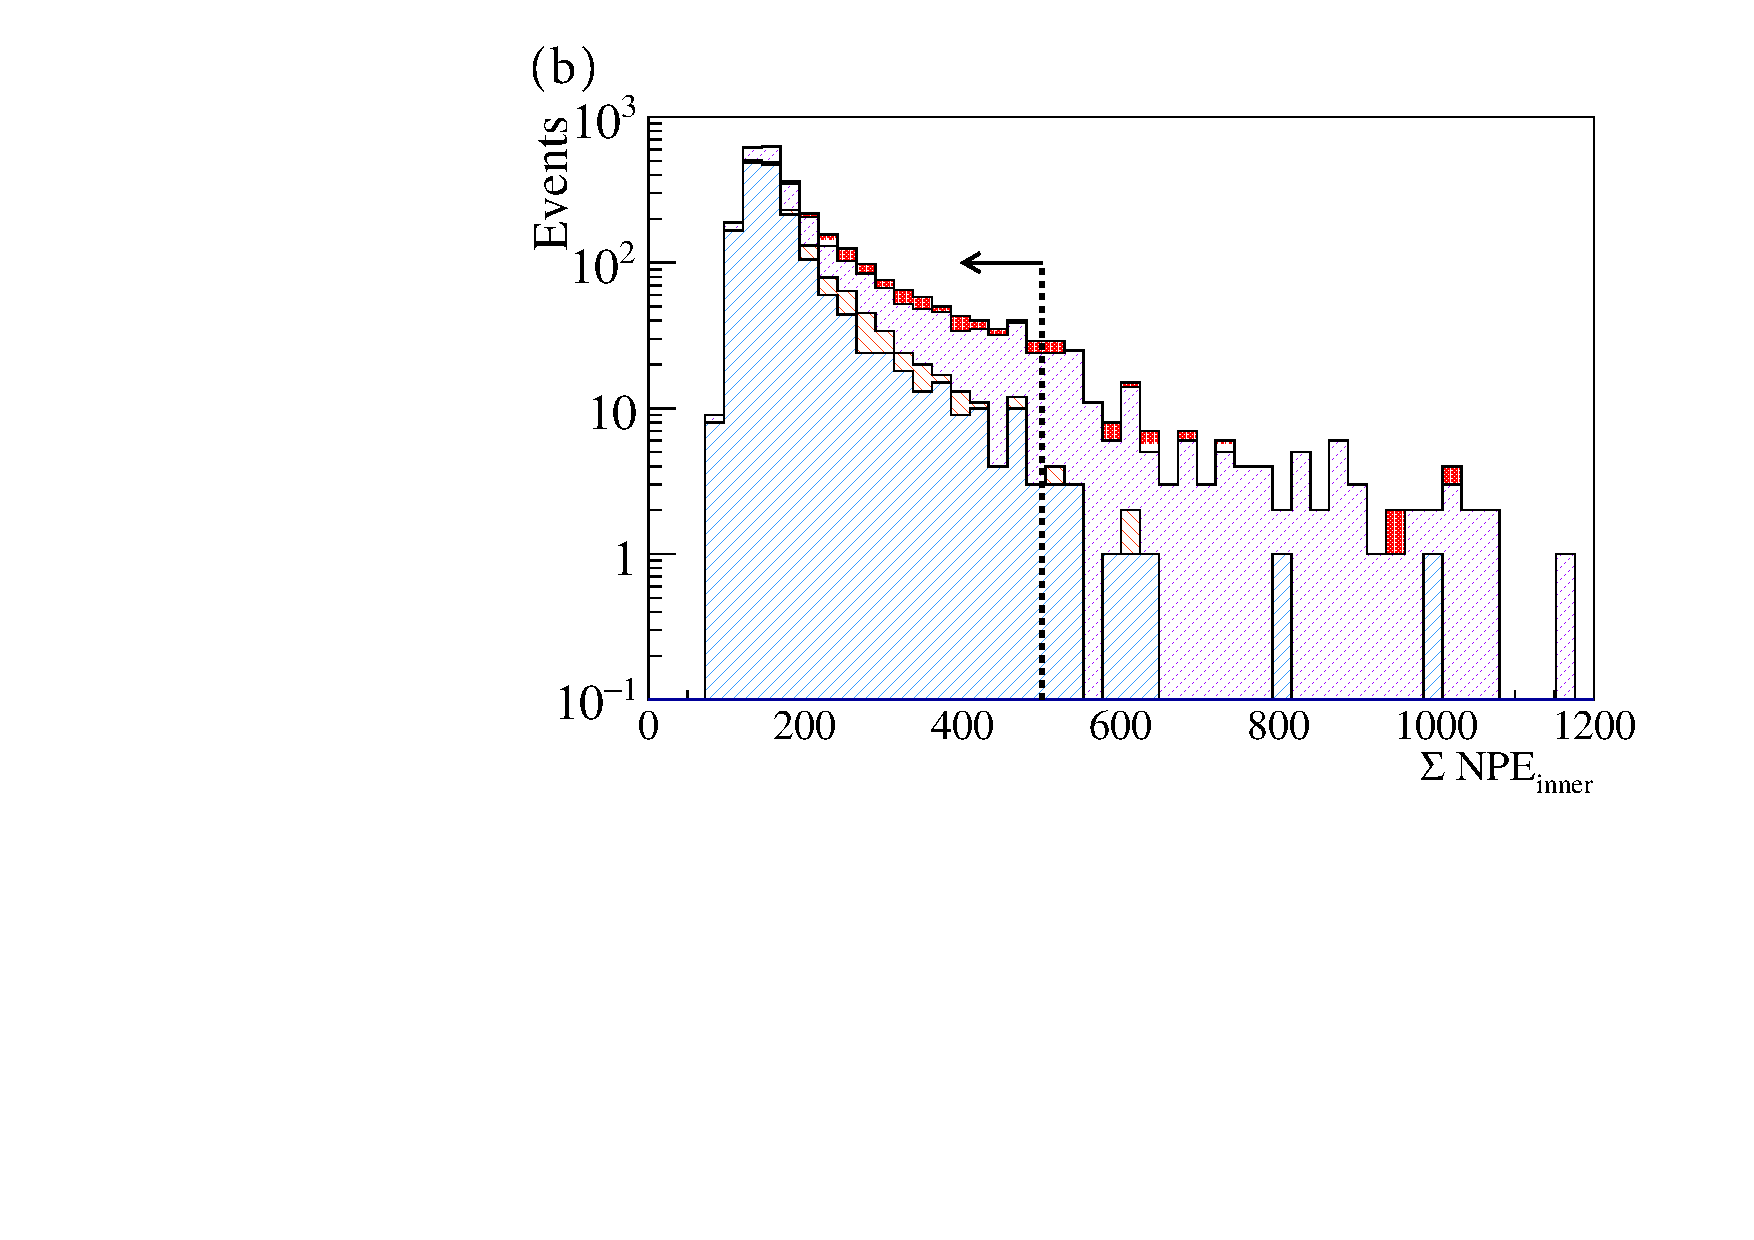
\includegraphics[width=0.6\columnwidth]{cosmic_labppo_clipping}
\caption{MC simulation of the summed PE distribution on the inner PMT group due to cosmic muon events with perfect rings (turquoise, right diagonal hatching), muon contamination (orange, left diagonal hatching), electron contamination (purple, right diagonal dashed hatching), and the total (red, solid).  (a) Water target, with water data overlaid to show the agreement, and (b) {\labppo} target.  The vertical black dashed line represents the chosen cut value, with arrows to illustrate the acceptance region. Figure from~\cite{chess_nim}.}
\label{f:clipMC}
\end{figure}

In water this total number of PE in the innermost PMTs is expected to be very low (consistent with noise), whereas in LS the total number of PE will be higher due to scintillation photons.  
However, as demonstrated in \Cref{f:clipMC}, a large fraction of follower events can still be removed with a high-charge cut.   
A cut was placed at a summed PE count of 40 for water and LAB targets, and 500 for {\labppo}.  
The cut value selected for a water target removes a large fraction of the remaining background events, with zero sacrifice in the control sample, and is expected to perform similarly for {\labppo} targets.

\section{Event-Level Analysis}\label{s:recon}

Time separation of the Cherenkov and scintillation photon populations is based on the hit-time residual distributions for each radial PMT grouping (inner, middle and outer).  
The hit-time residuals are evaluated as the PMT hit times with respect to the event time, corrected by per-channel delays (\Cref{s:delay}) and by the photon ToF.  
The ToF depends on the distance between the target and the PMTs, and on the refractive indices of the different media. 
It is estimated for each PMT radial group to be $626$~ps, $536$~ps and $473$~ps for the inner, middle and outer PMT rings, respectively.
In this way, the hit-time-residual distributions of each radial grouping represents the photon emission times in three angular bins with respect to the muon direction.

Event time is defined as the time at which the muon travels through the center of the target, and must be determined to high precision such that hit-time residuals from many events can be compared
The most straightforward event time would be with respect to the cosmic muon tags, however, given the slowness of the scintillator emission and poorer TTS of the tag PMTs, this time is not precise enough.
A higher precision event time is reconstructed from each event as the median of the hit-time residuals for the four earliest hits.
This provides a robust time reference since the prompt hits are due to Cherenkov light, which has a very sharp time profile.
A comparison of using this definition of event time and event time defined with respect to the muon tag is shown in \Cref{f:smear}, overlaid with the MC prediction in each case.  

The residual distribution with respect to the muon tag time is extremely well reproduced by the MC, demonstrating the precision of the model.
The simulation slightly under predicts the width of the higher precision distribution of residuals with respect to the reconstructed event time.  
This is most likely due to an underestimation of the PMT TTS used in the MC, so an additional time uncertainty of $\sigma=214$~ps is included in the simulation, resulting in the corrected results from \Cref{f:smear}.

\begin{figure}
\centering
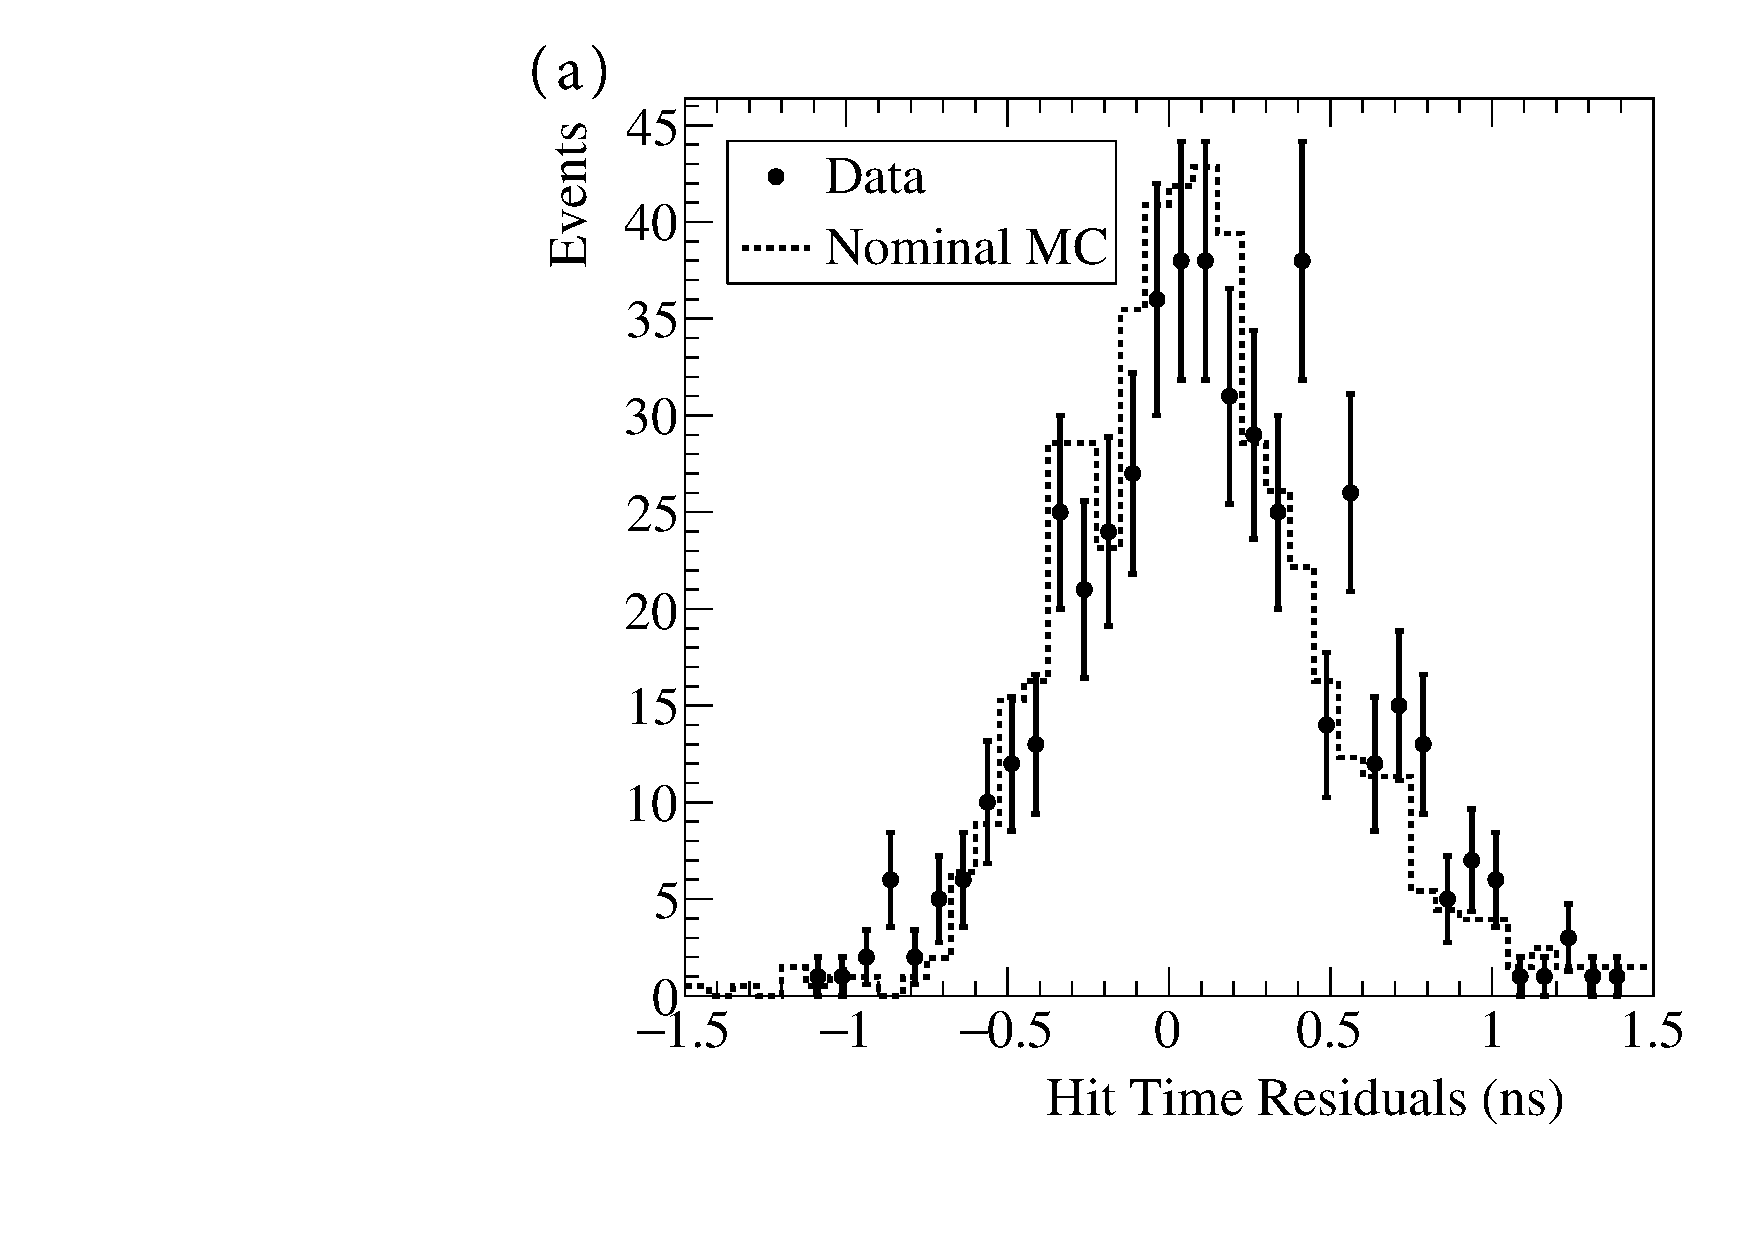
\includegraphics[width=0.49\columnwidth]{cosmic_water_timeres_trtime_dt_mc}
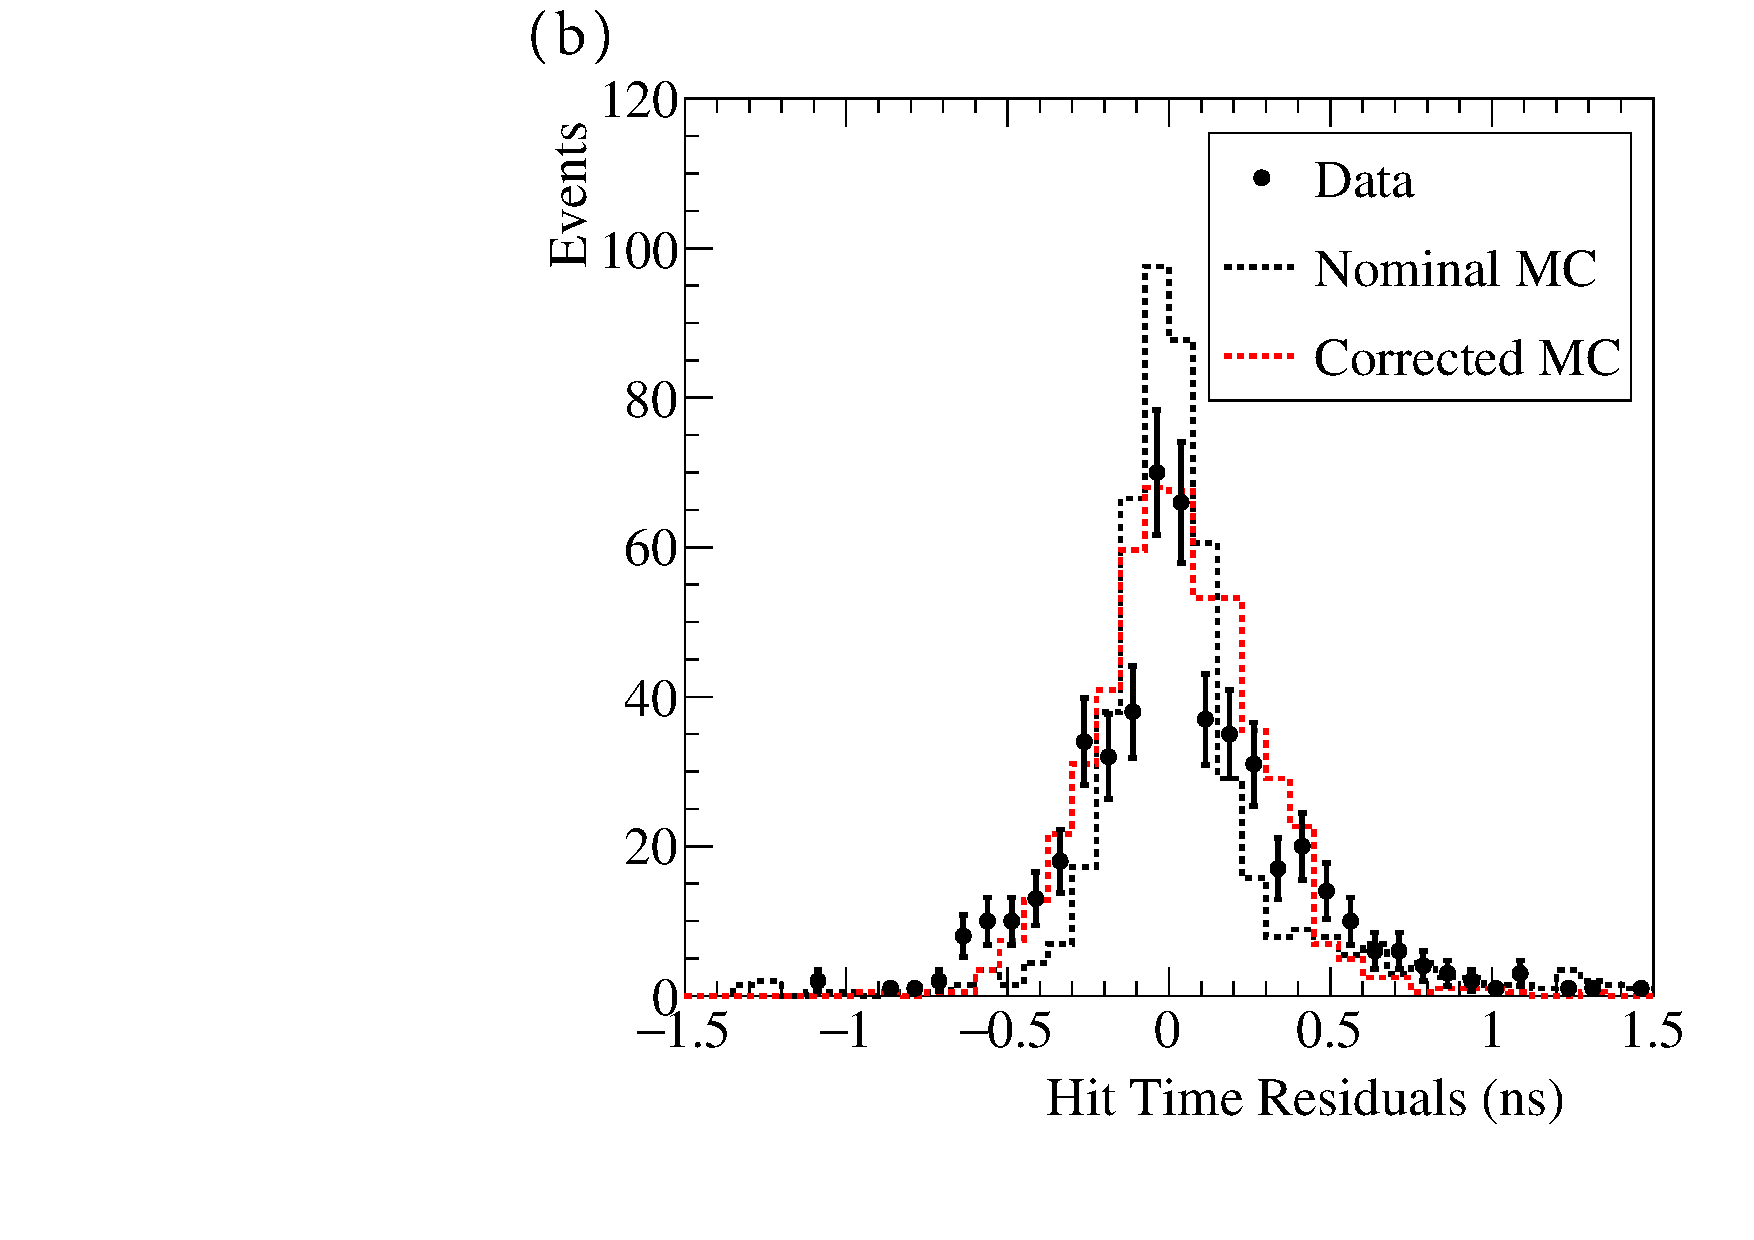
\includegraphics[width=0.49\columnwidth]{cosmic_water_timeres_dt_mc_smear}
\caption{Distribution of hit-time residuals for ring candidate events in water for middle PMTs, where the Cherenkov ring is expected. Data points are shown with statistical errors, with the MC prediction overlaid (dashed lines). 
(a) Hit times with respect to the lower muon tag time and (b) hit times with respect to the reconstructed event time.
Figure from~\cite{chess_nim}.}
\label{f:smear}
\end{figure}

\subsection{Figures of Merit}

The separation can be quantified by taking the ratio of hit counts between the outer PMTs (fast Cherenkov photons) and the middle and inner PMTs (slower scintillation photons).  
A time cut ($t < t_c$) is optimized in order to maximize separation.  
The efficiency of identifying Cherenkov hits is defined as the fraction of outer PMT hits that occur before $t_c$.  
The scintillation contamination  is given by the fraction of hits occurring before $t_c$ that are due to scintillation, \textit{i.e.} hits with $t < t_c$ on inner and middle PMT groupings for pure LAB and {\labppo} targets (inner and outer PMTs for water or WbLS targets). 

Charge separation can be achieved by taking the ratio of charge in a prompt 5~ns window to that in the full event window for each hit PMT and comparing this for the different radial PMT groupings.  
The separation is defined in an analogous manner to that for time: a threshold is optimized to maximize the Cherenkov hit detection efficiency and minimize scintillation contamination.  

\clearpage

\section{Cherenkov Ring-Imaging in Water}

\label{sec:water}

After application of the event selection criteria, 137 ring candidates were selected in the water dataset.
The number of detected PEs and first photon hit-time residuals for a typical event are shown in \Cref{fig:cosmics_water_ring_candidate}. 
The averages across the dataset for both the number of detected PEs per PMT and the hit-time residuals are shown in \Cref{fig:cosmics_water_npes}.
Both cases show a clear ring structure, indicating that CHESS is imaging Cherenkov rings and that the event selection criteria produce a clean population of events. 


\begin{figure}
\centering
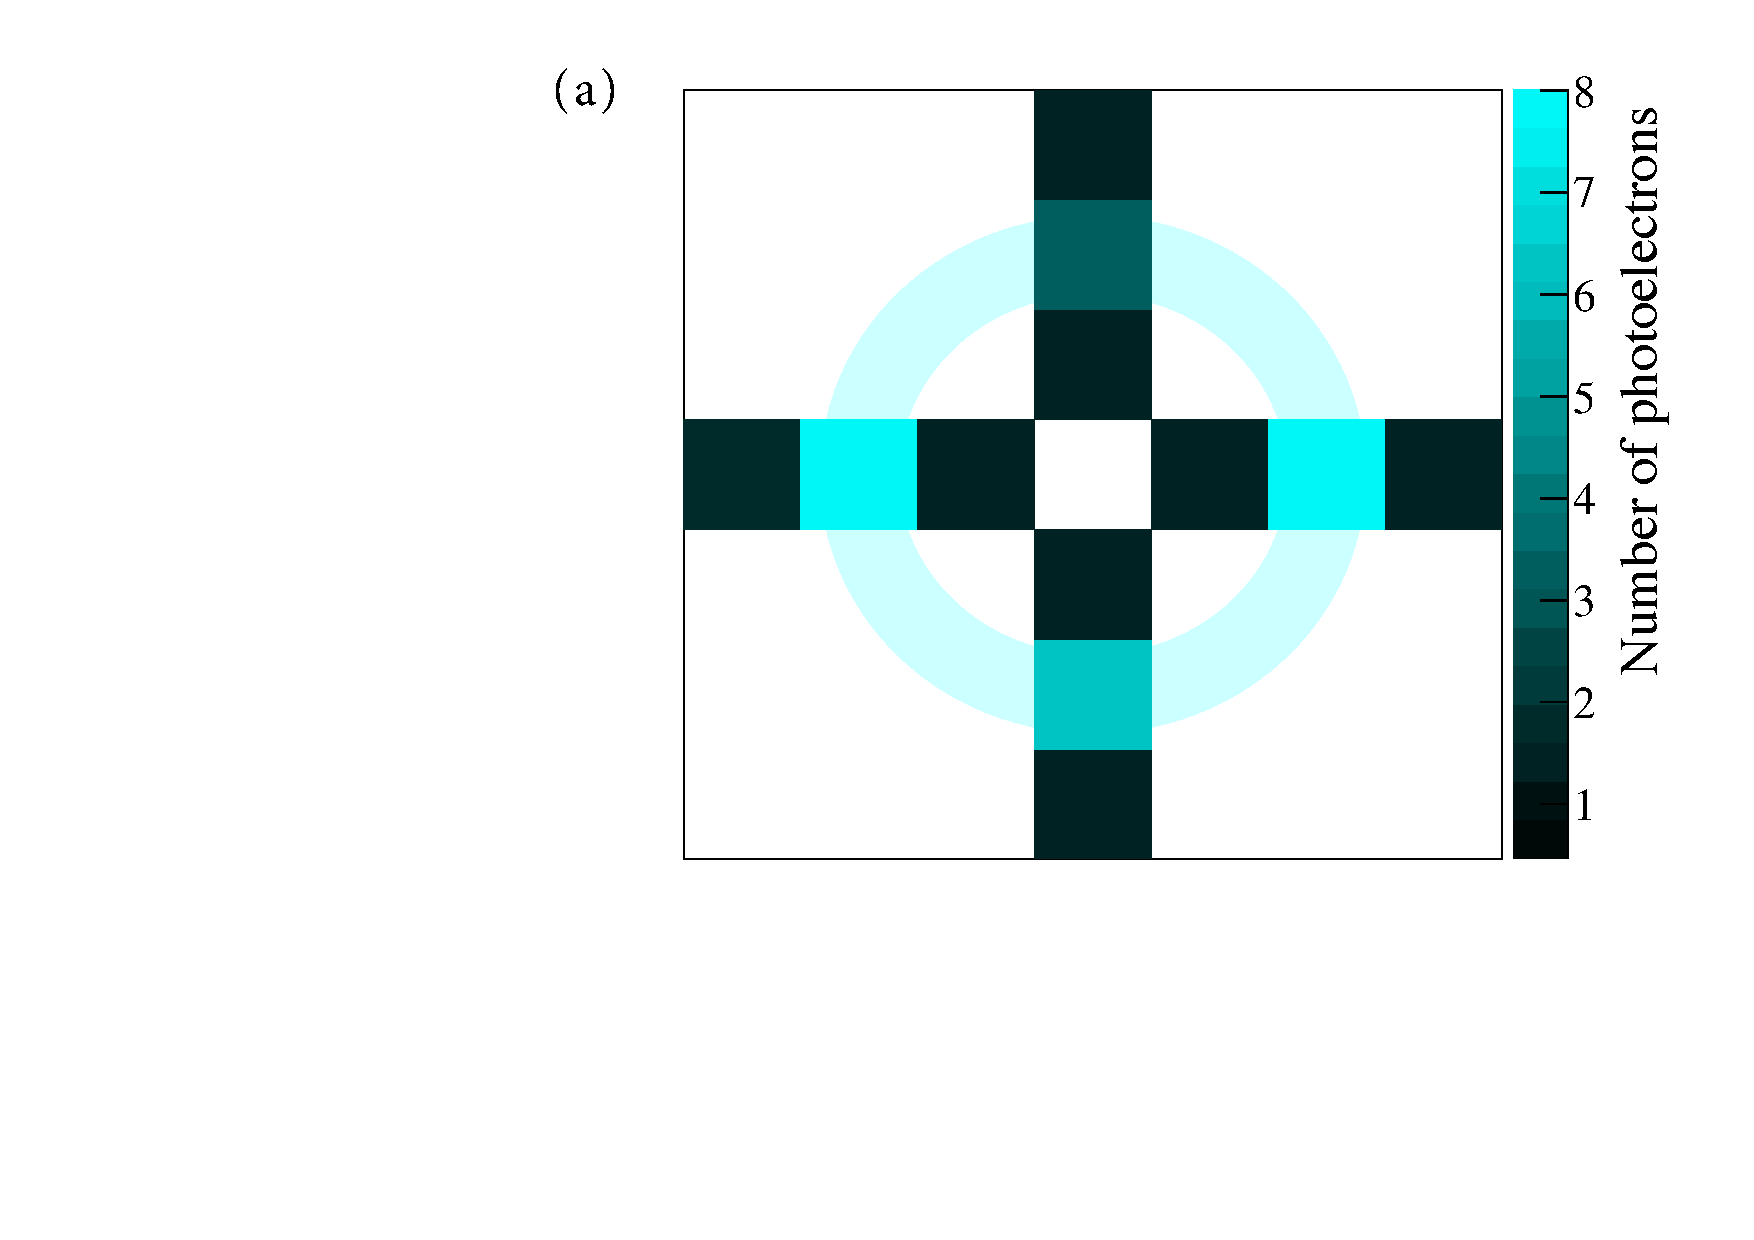
\includegraphics[width=0.47\columnwidth]{cosmic_water_ringcandidate_npe_dt}
\hfill
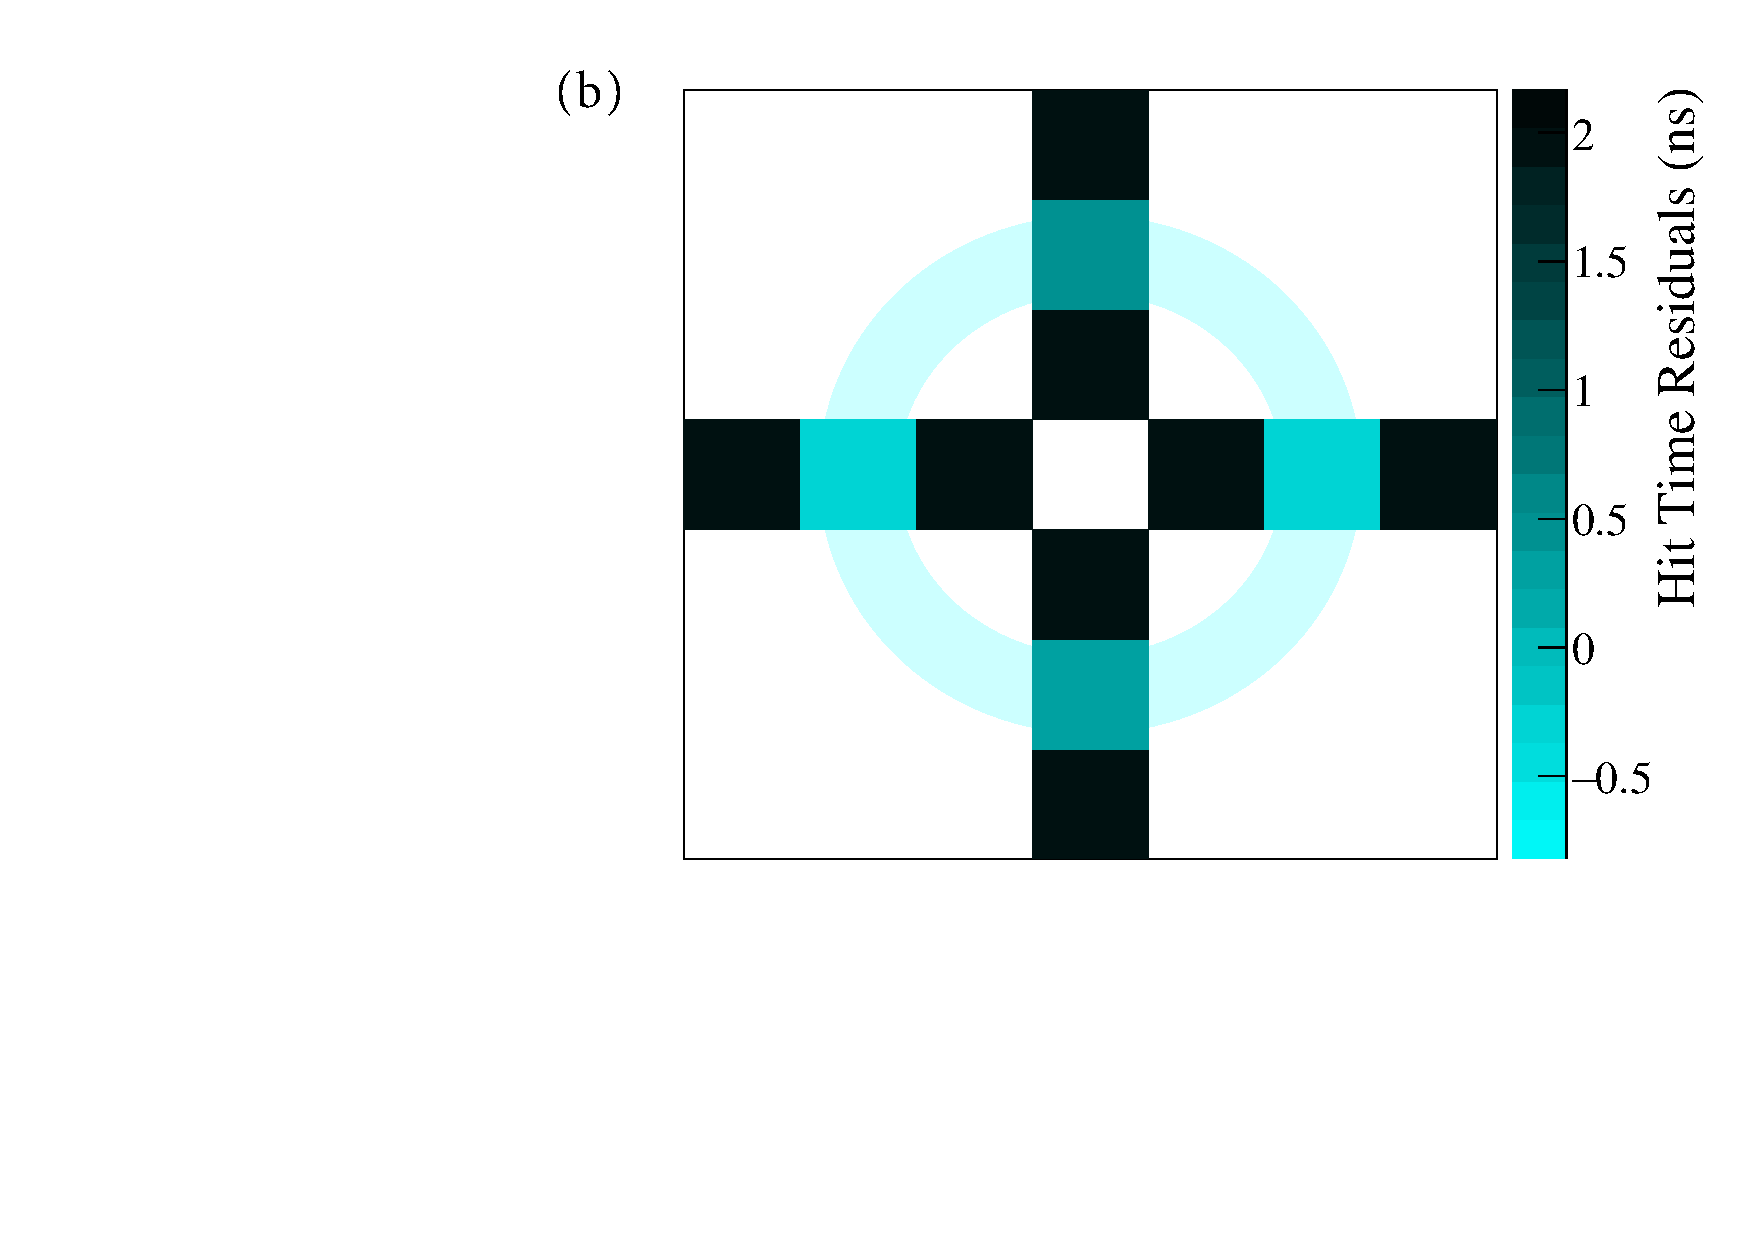
\includegraphics[width=0.47\columnwidth]{cosmic_water_ringcandidate_time_dt}
\caption{Typical ring event in the water dataset. (a) Estimated number of detected PEs and (b) hit-time residuals. Figure from~\cite{chess_nim}.}
\label{fig:cosmics_water_ring_candidate}
\end{figure}


\begin{figure}
\centering
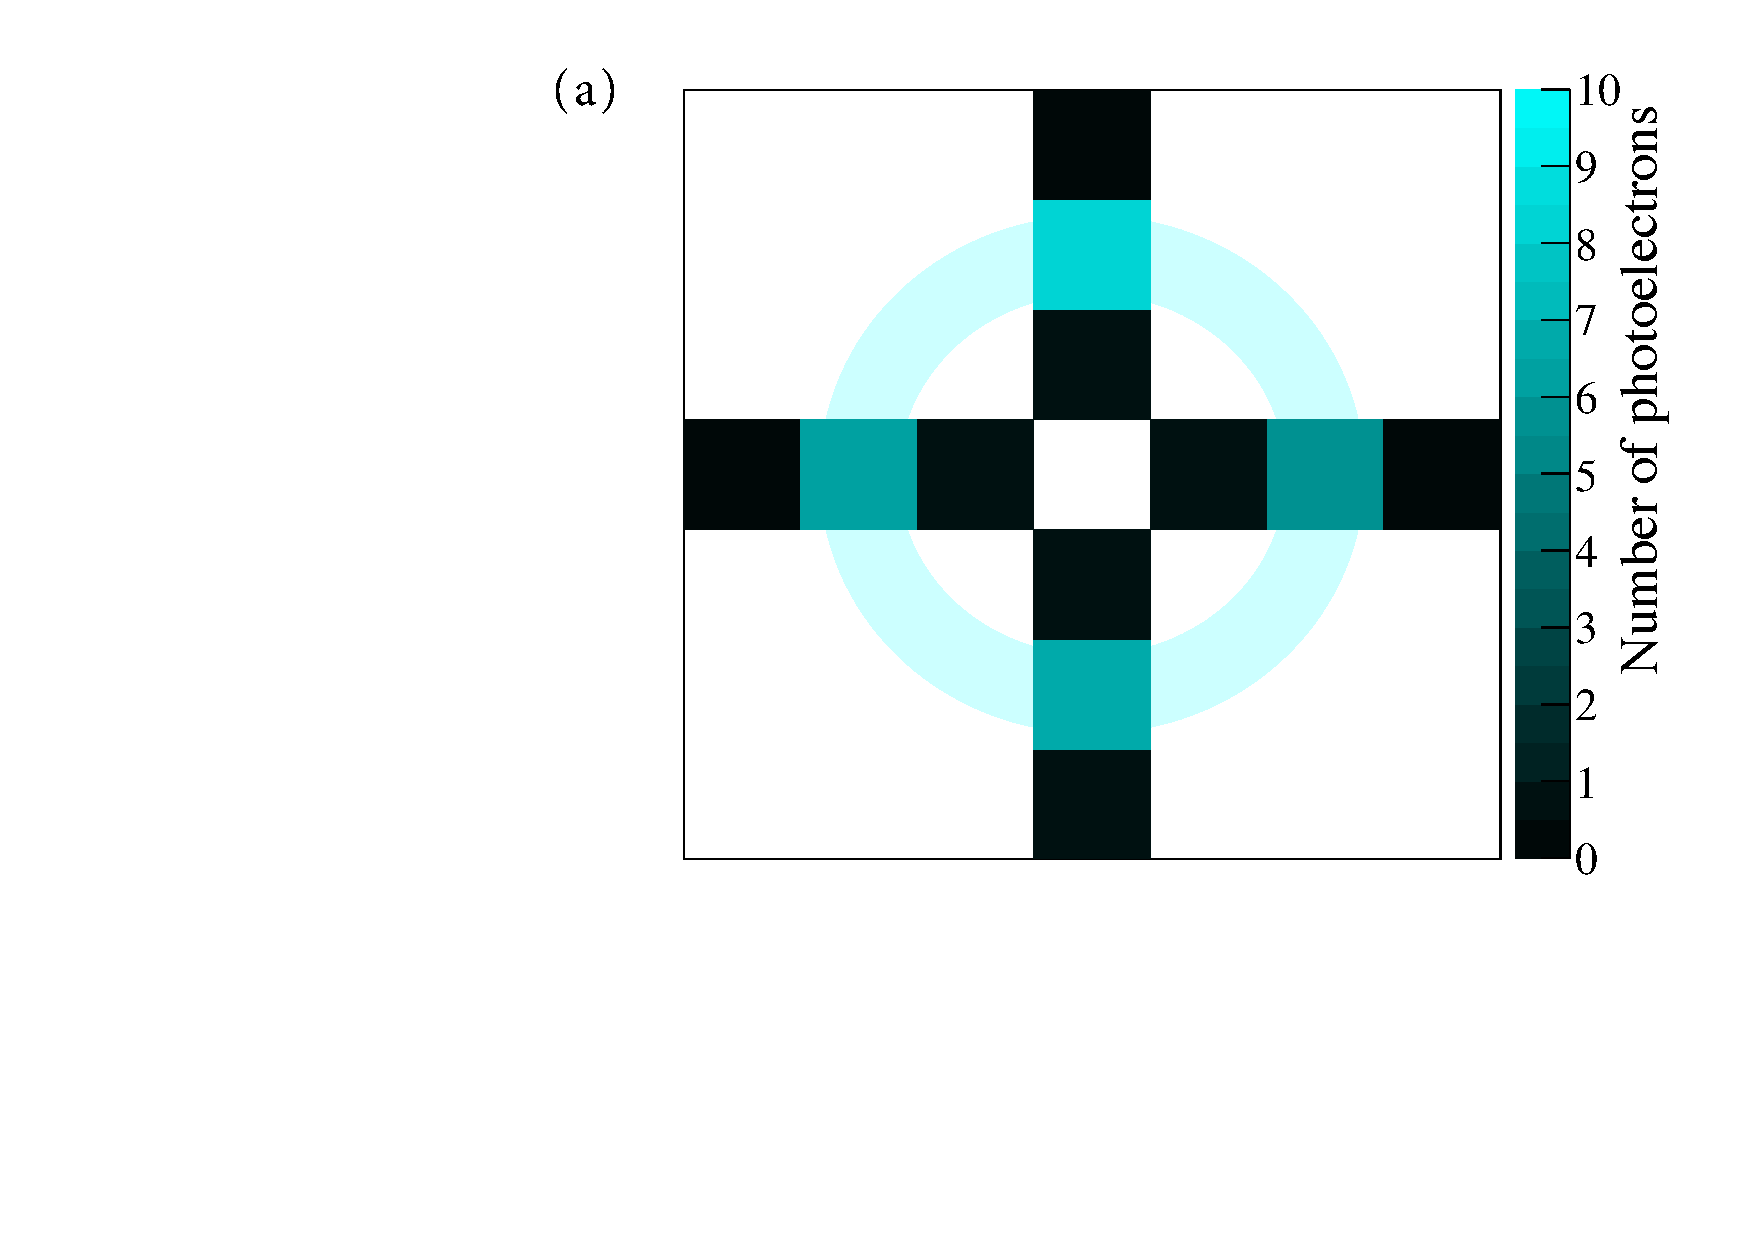
\includegraphics[width=0.47\columnwidth]{cosmic_water_ringnpe_dt}
\hfill
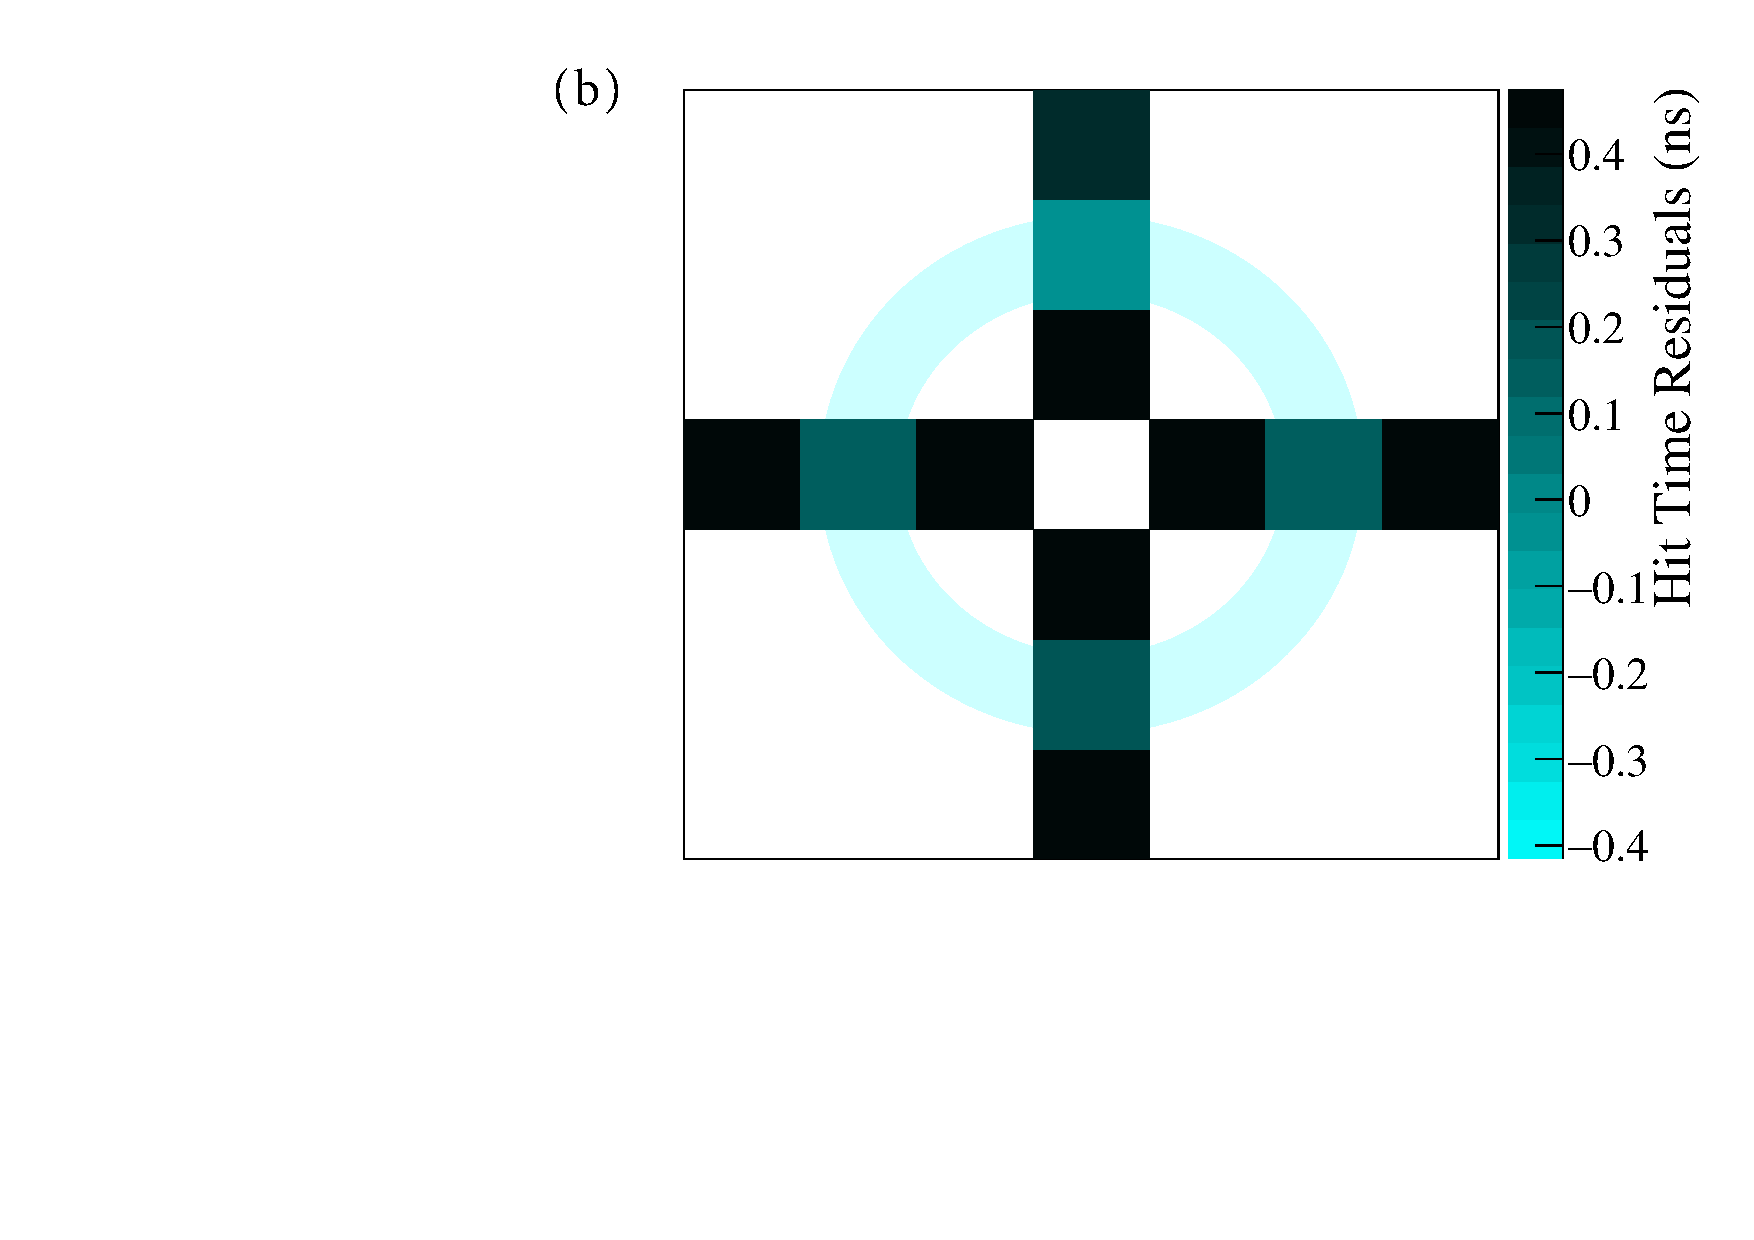
\includegraphics[width=0.47\columnwidth]{cosmic_water_ringtime_dt}
\caption{(a) Averaged number of detected PE and (b) averaged first-photon hit-time residual per individual PMT for ring candidates in water data. Figure from~\cite{chess_nim}.}
\label{fig:cosmics_water_npes}
\end{figure}


The distributions of hit-time residuals for each PMT radial group (inner, middle and outer PMTs) are shown in \Cref{fig:cosmics_water}, with the MC prediction overlaid. 
The Cherenkov ring is only expected to hit the middle PMTs with a water target, and this is clearly demonstrated.
Importantly, the MC accurately predicts the hit-time residual distribution for the Cherenkov hits. 


\begin{figure}
\centering
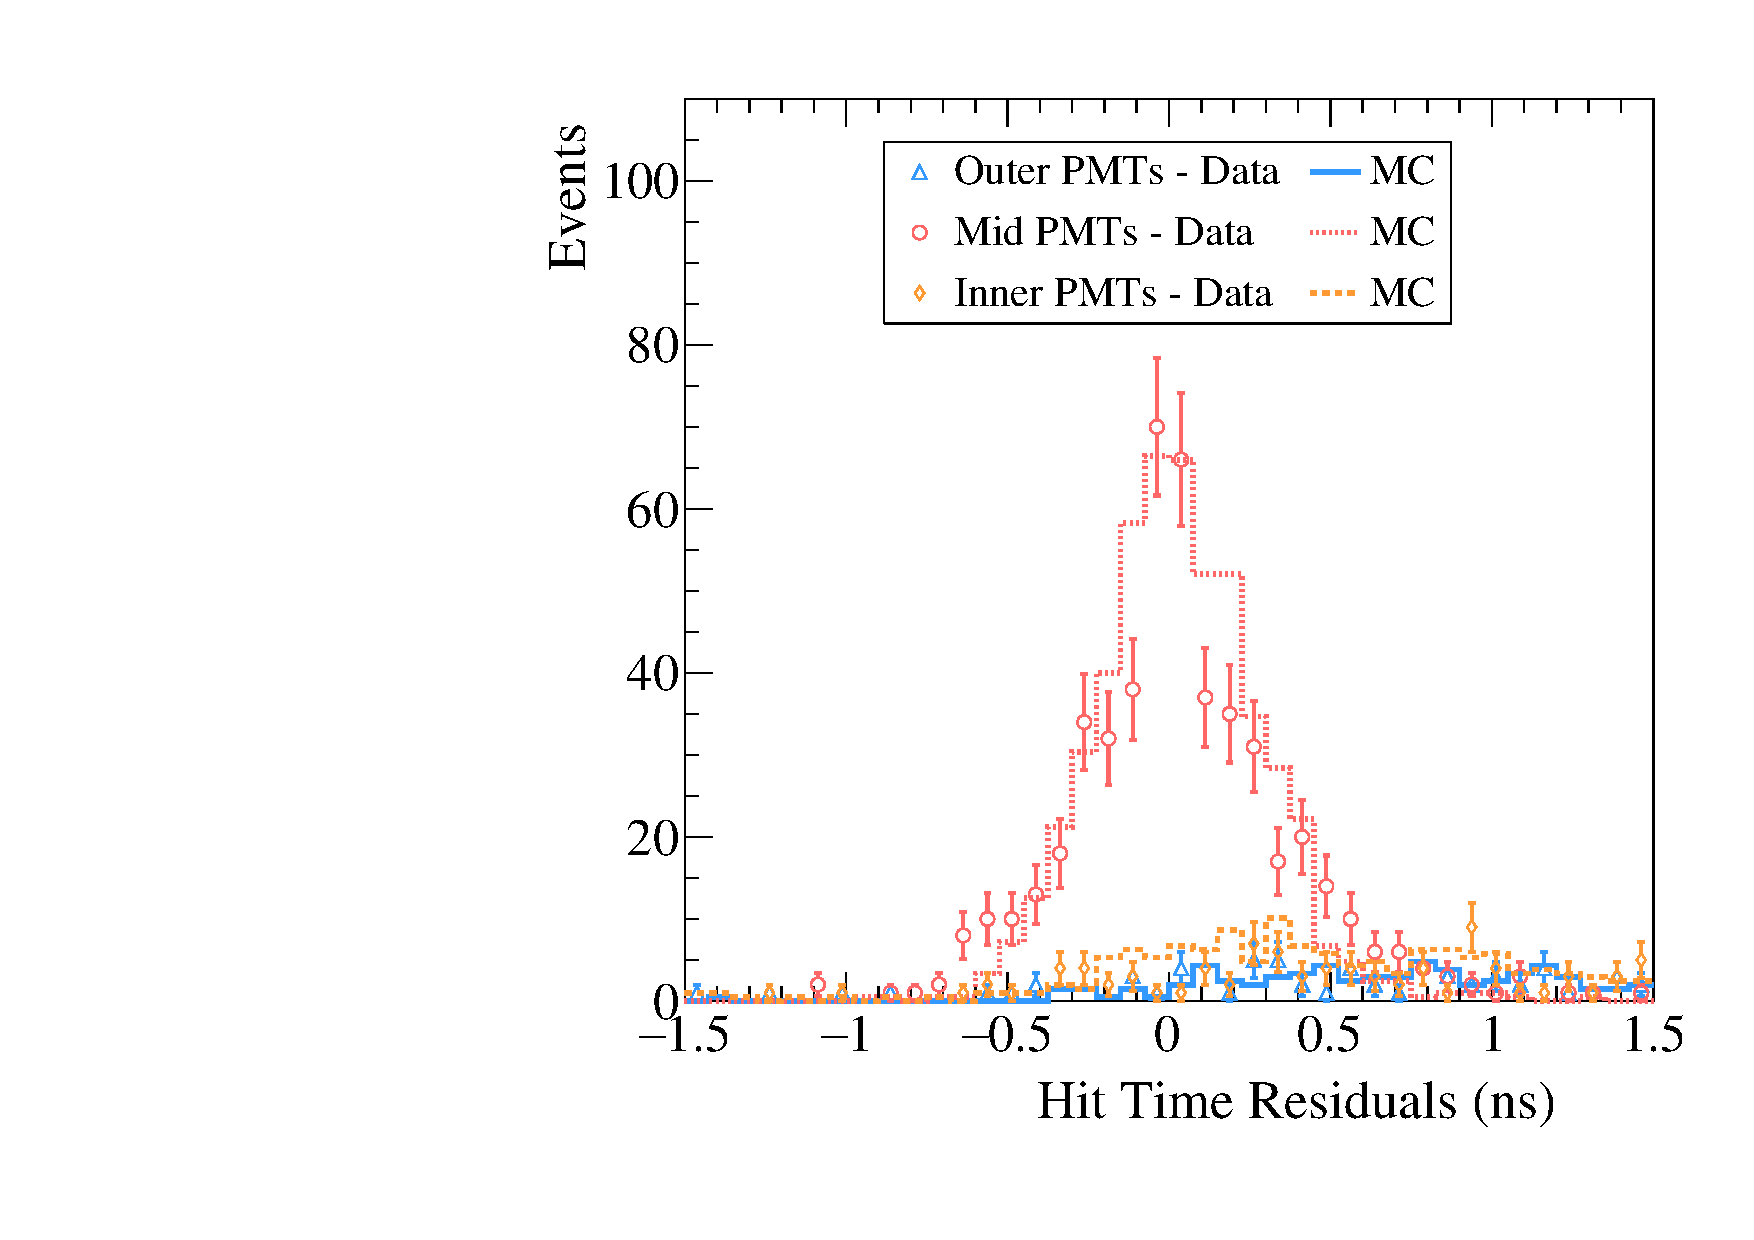
\includegraphics[width=0.7\columnwidth]{cosmic_water_25pctpe_time_smear}
\caption{Distribution of hit-time residuals for ring candidate events in water for each PMT radial group. Data points are shown with statistical errors, with the MC prediction overlaid (dashed lines). Figure from~\cite{chess_nim}.}
\label{fig:cosmics_water}
\end{figure}


The sharp time distribution of Cherenkov light provides a way to estimate the time resolution of CHESS.
Assuming a delta function for the Cherenkov profile, the time resolution of CHESS is the width of the measured hit-time residual distribution: $338\pm 12$~ps FWHM. 
This is appropriately close to the manufacturer estimate of the PMT TTS: 300~ps FWHM. 

\clearpage

\section{LAB Results}

\label{sec:lab}

Prior to moving to {\labppo}, pure LAB was deployed. 
The PPO component enhances the light yield significantly, so LAB by itself is expected to have low scintillation light yield, and perhaps a visible Cherenkov ring geometry.
After applying event selection criteria, $117$ ring candidates were identified in the LAB dataset. 
An example event is shown in \Cref{fig:lab_ring} for both time and charge, with the average across the dataset shown in \Cref{fig:lab2}. 
A clear ring structure can be observed in both cases. 

\begin{figure}
\centering
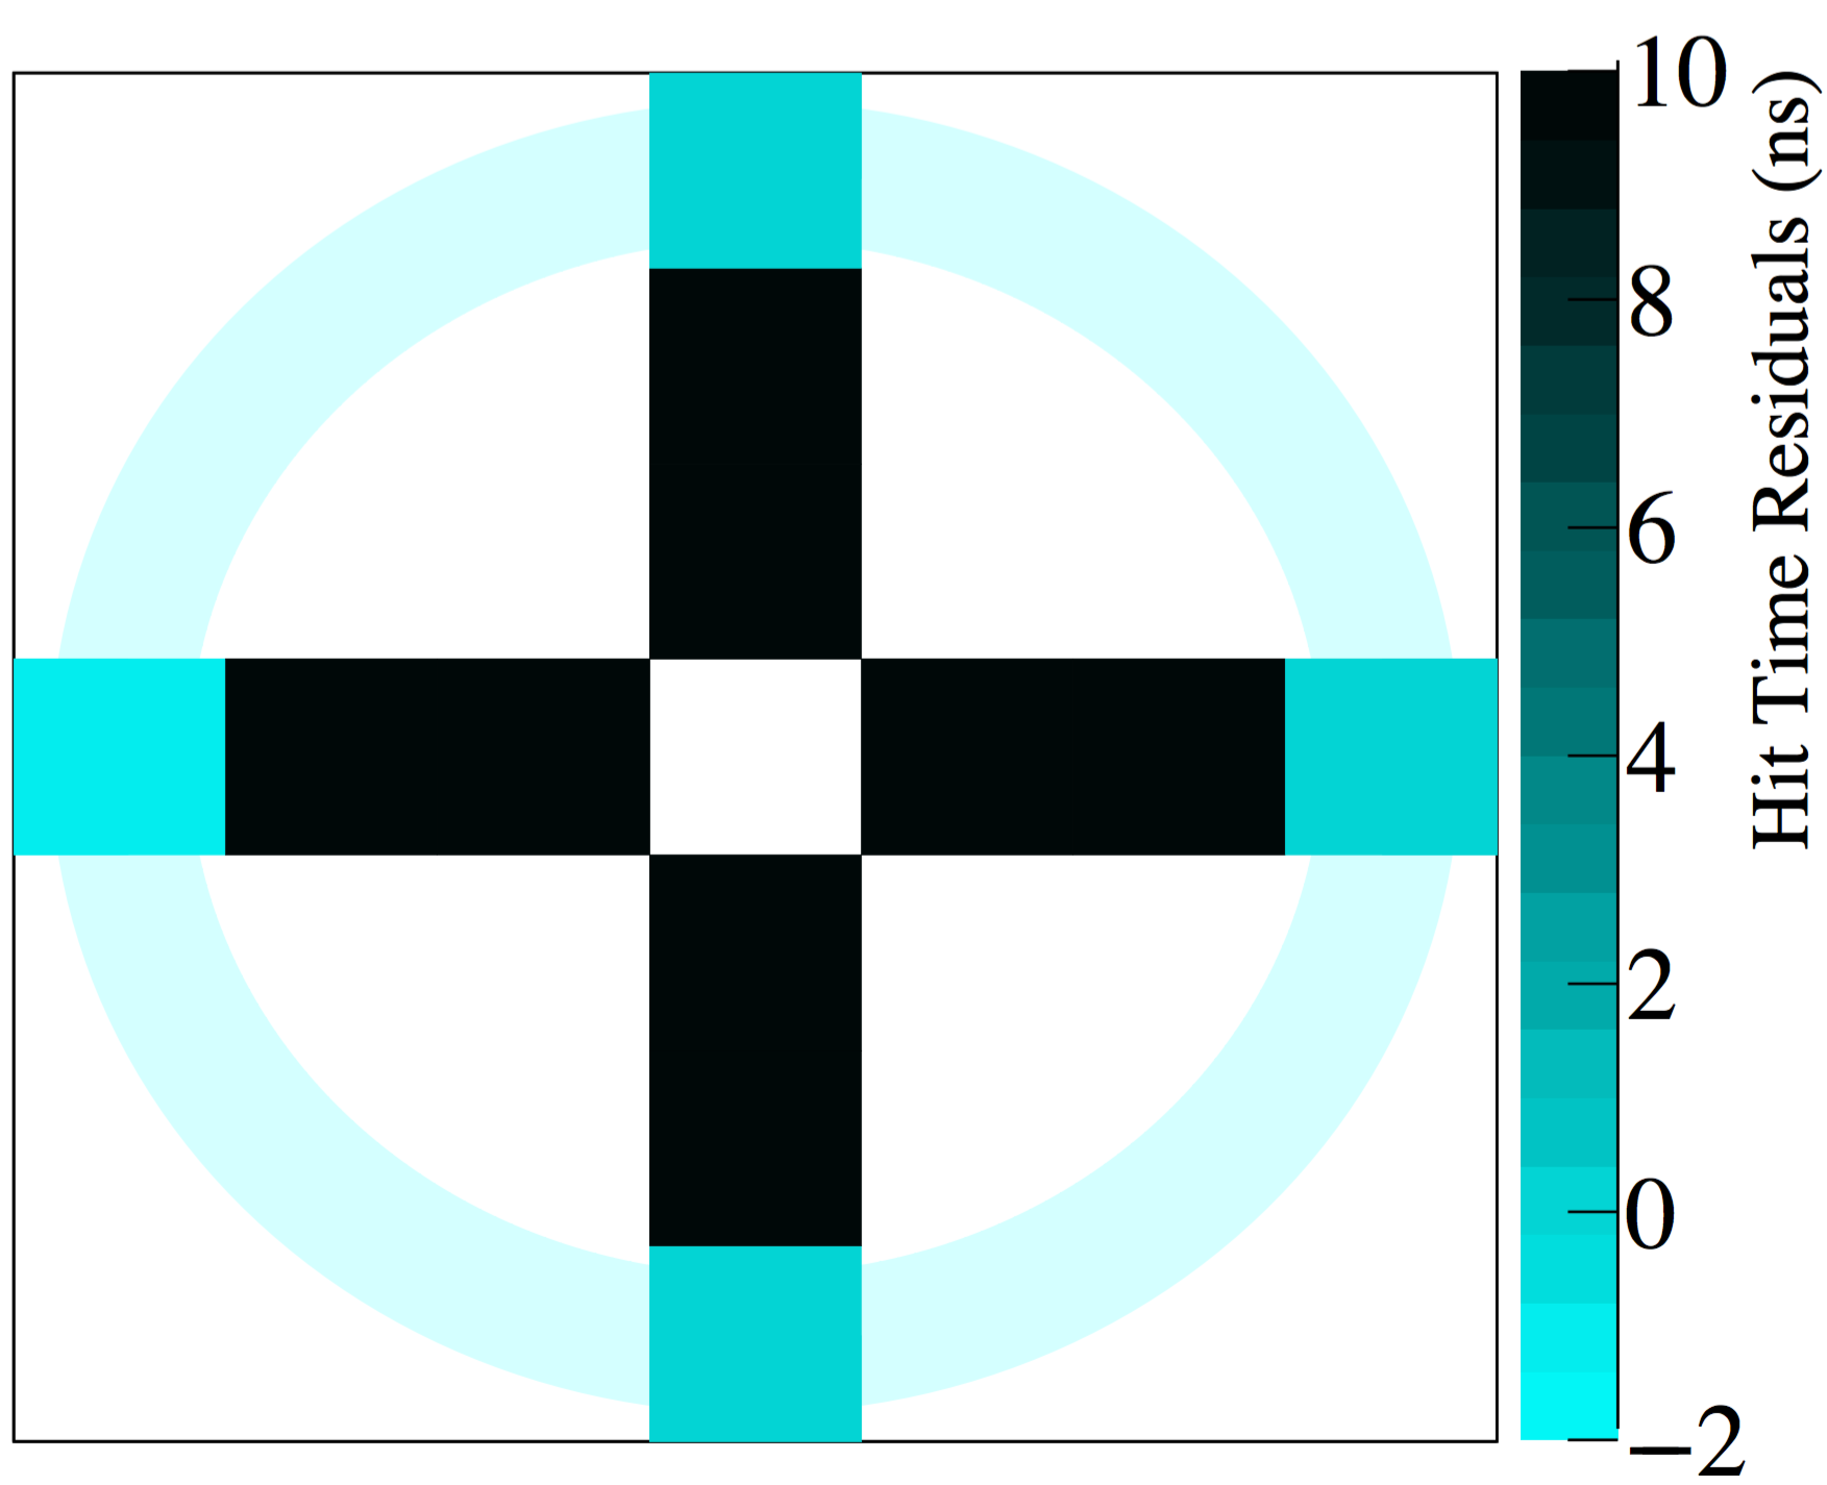
\includegraphics[width=0.47\columnwidth]{cosmic_lab_ringcandidate_time_dt}
\hfill
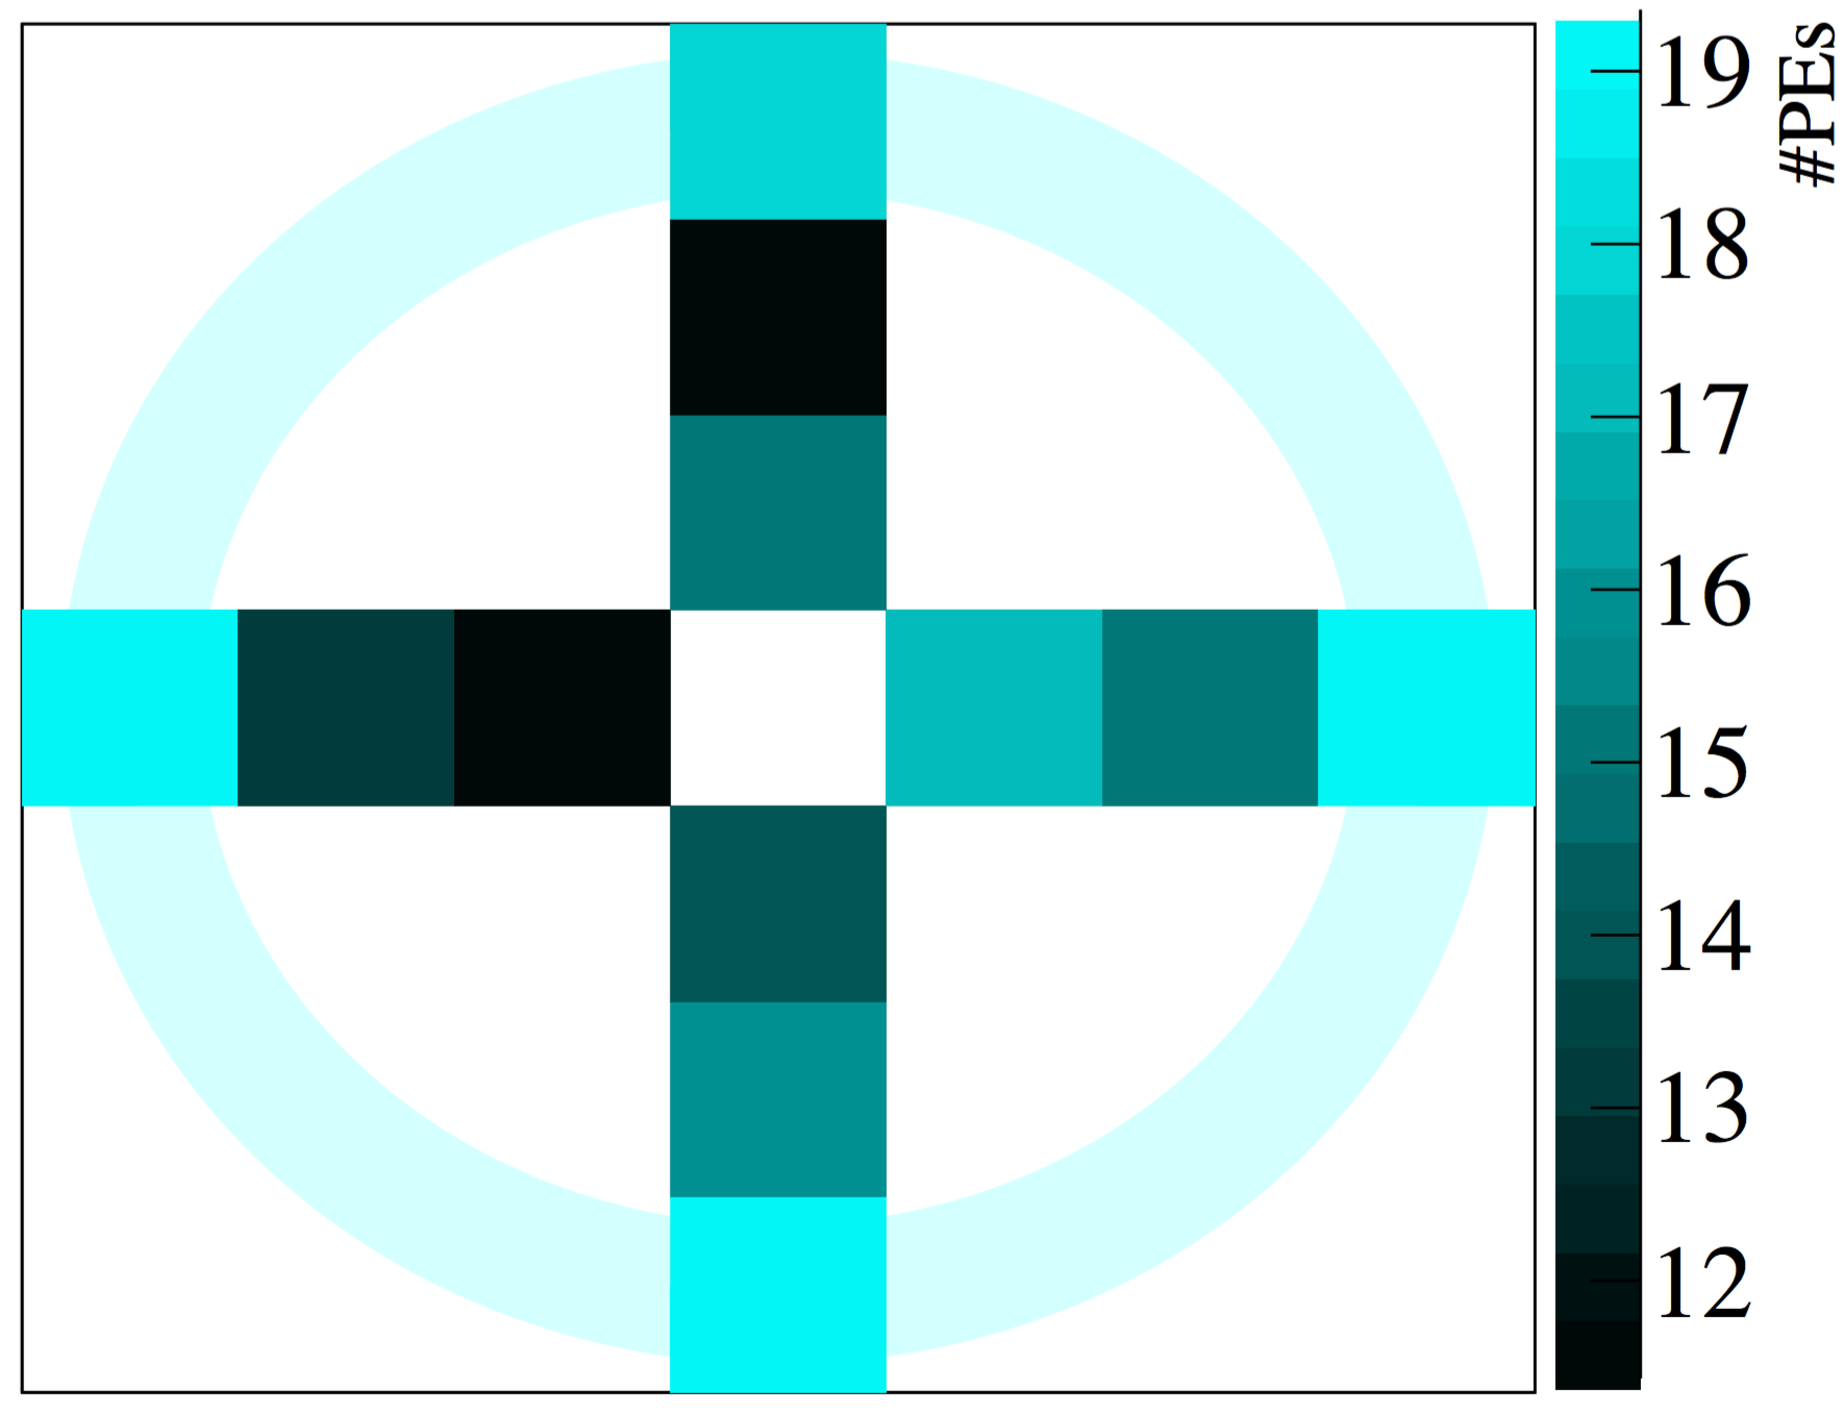
\includegraphics[width=0.47\columnwidth]{cosmic_lab_ringcandidate_npe_dt}
\caption{A single ring candidate event in LAB. Hit-time residual (left) and number of PE versus PMT position (right). Figure from~\cite{chess_lab}.}
\label{fig:lab_ring}
\end{figure}

\begin{figure}
\centering
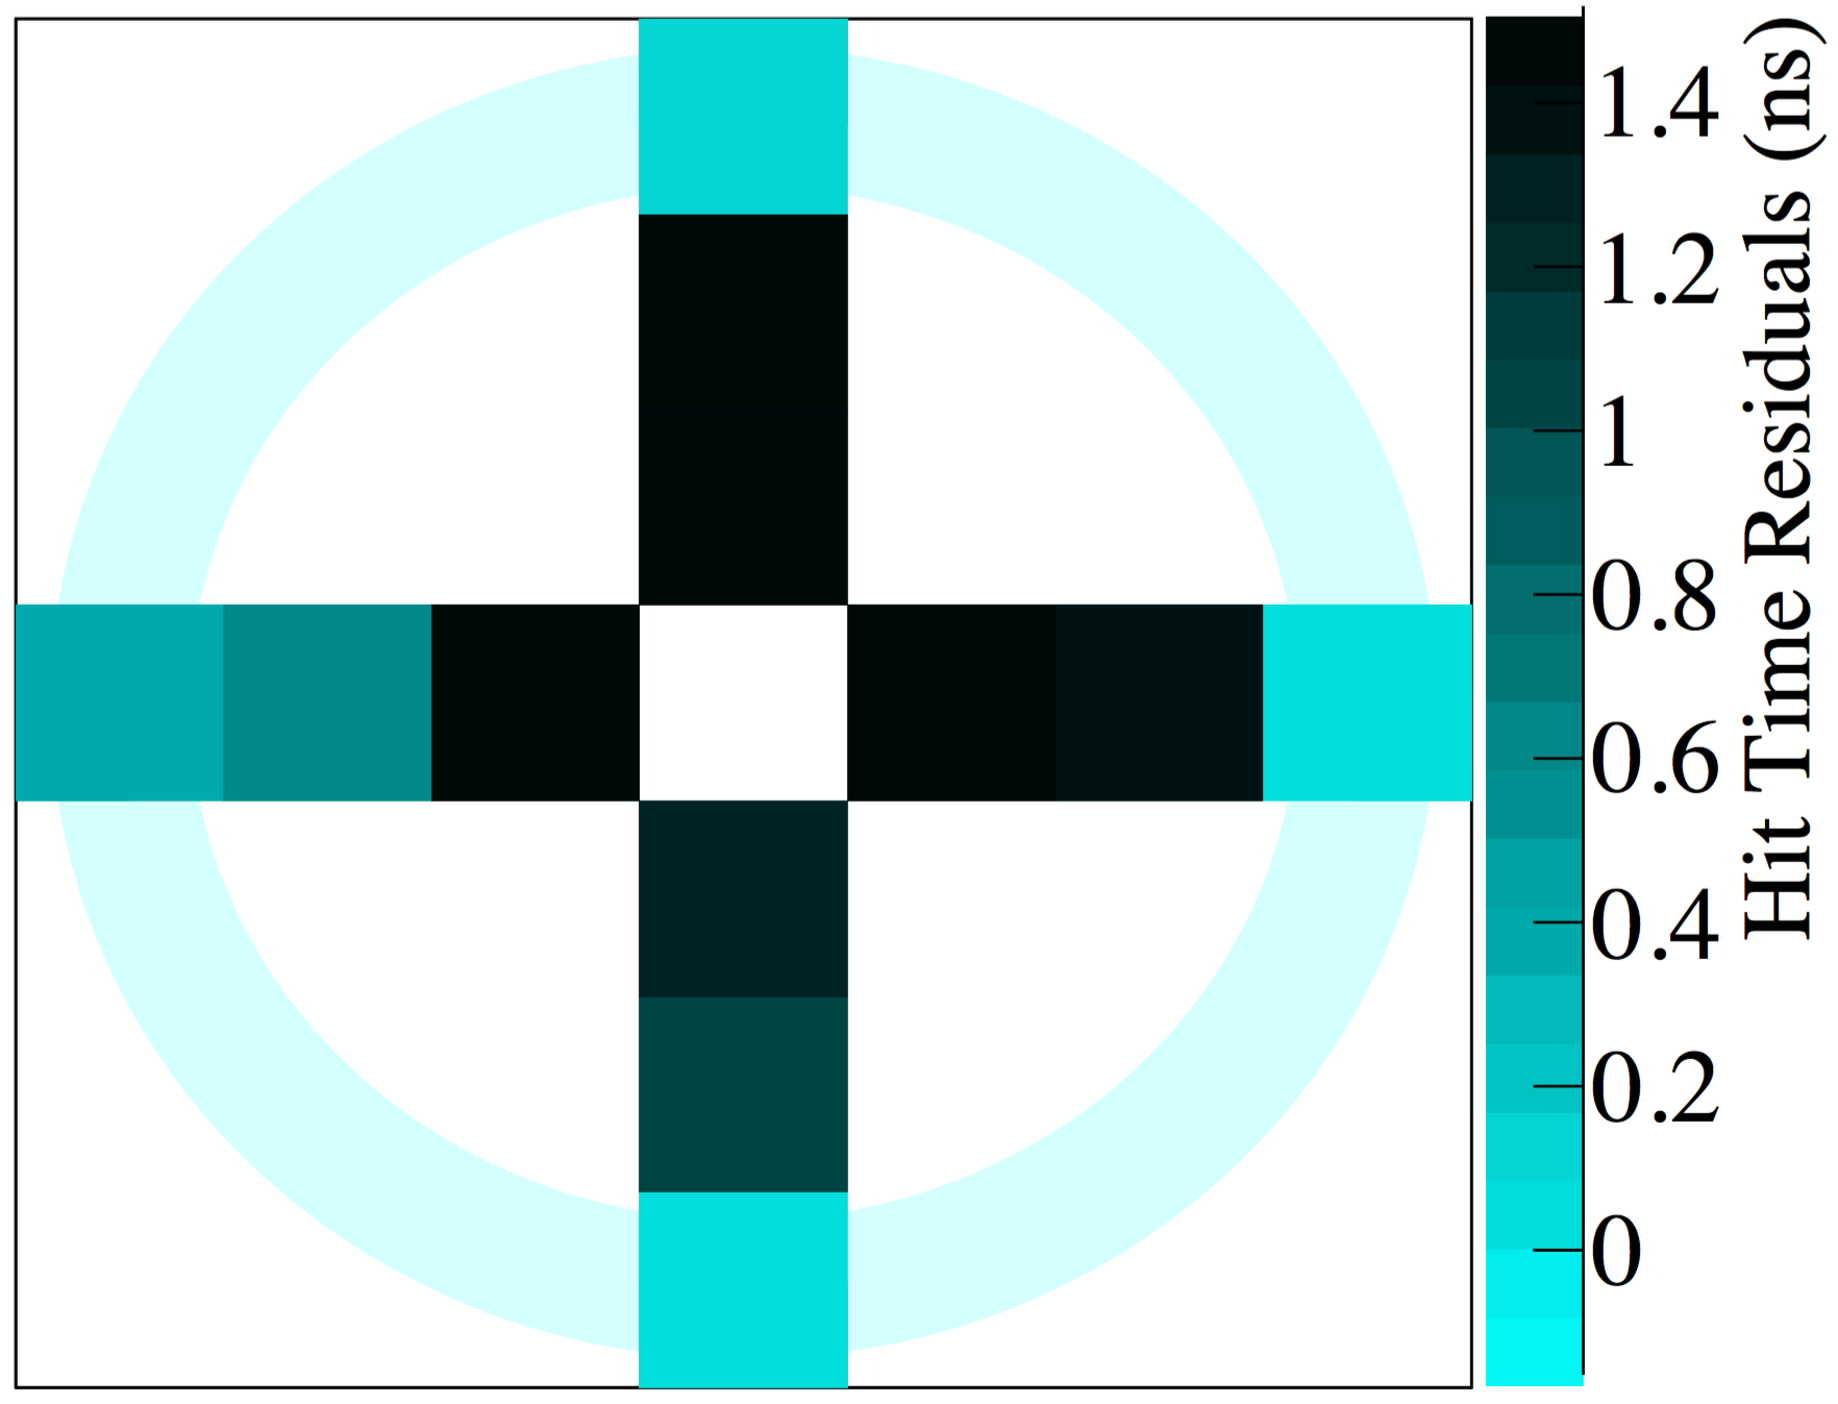
\includegraphics[width=0.47\columnwidth]{cosmic_lab_ringtime_dt}
\hfill
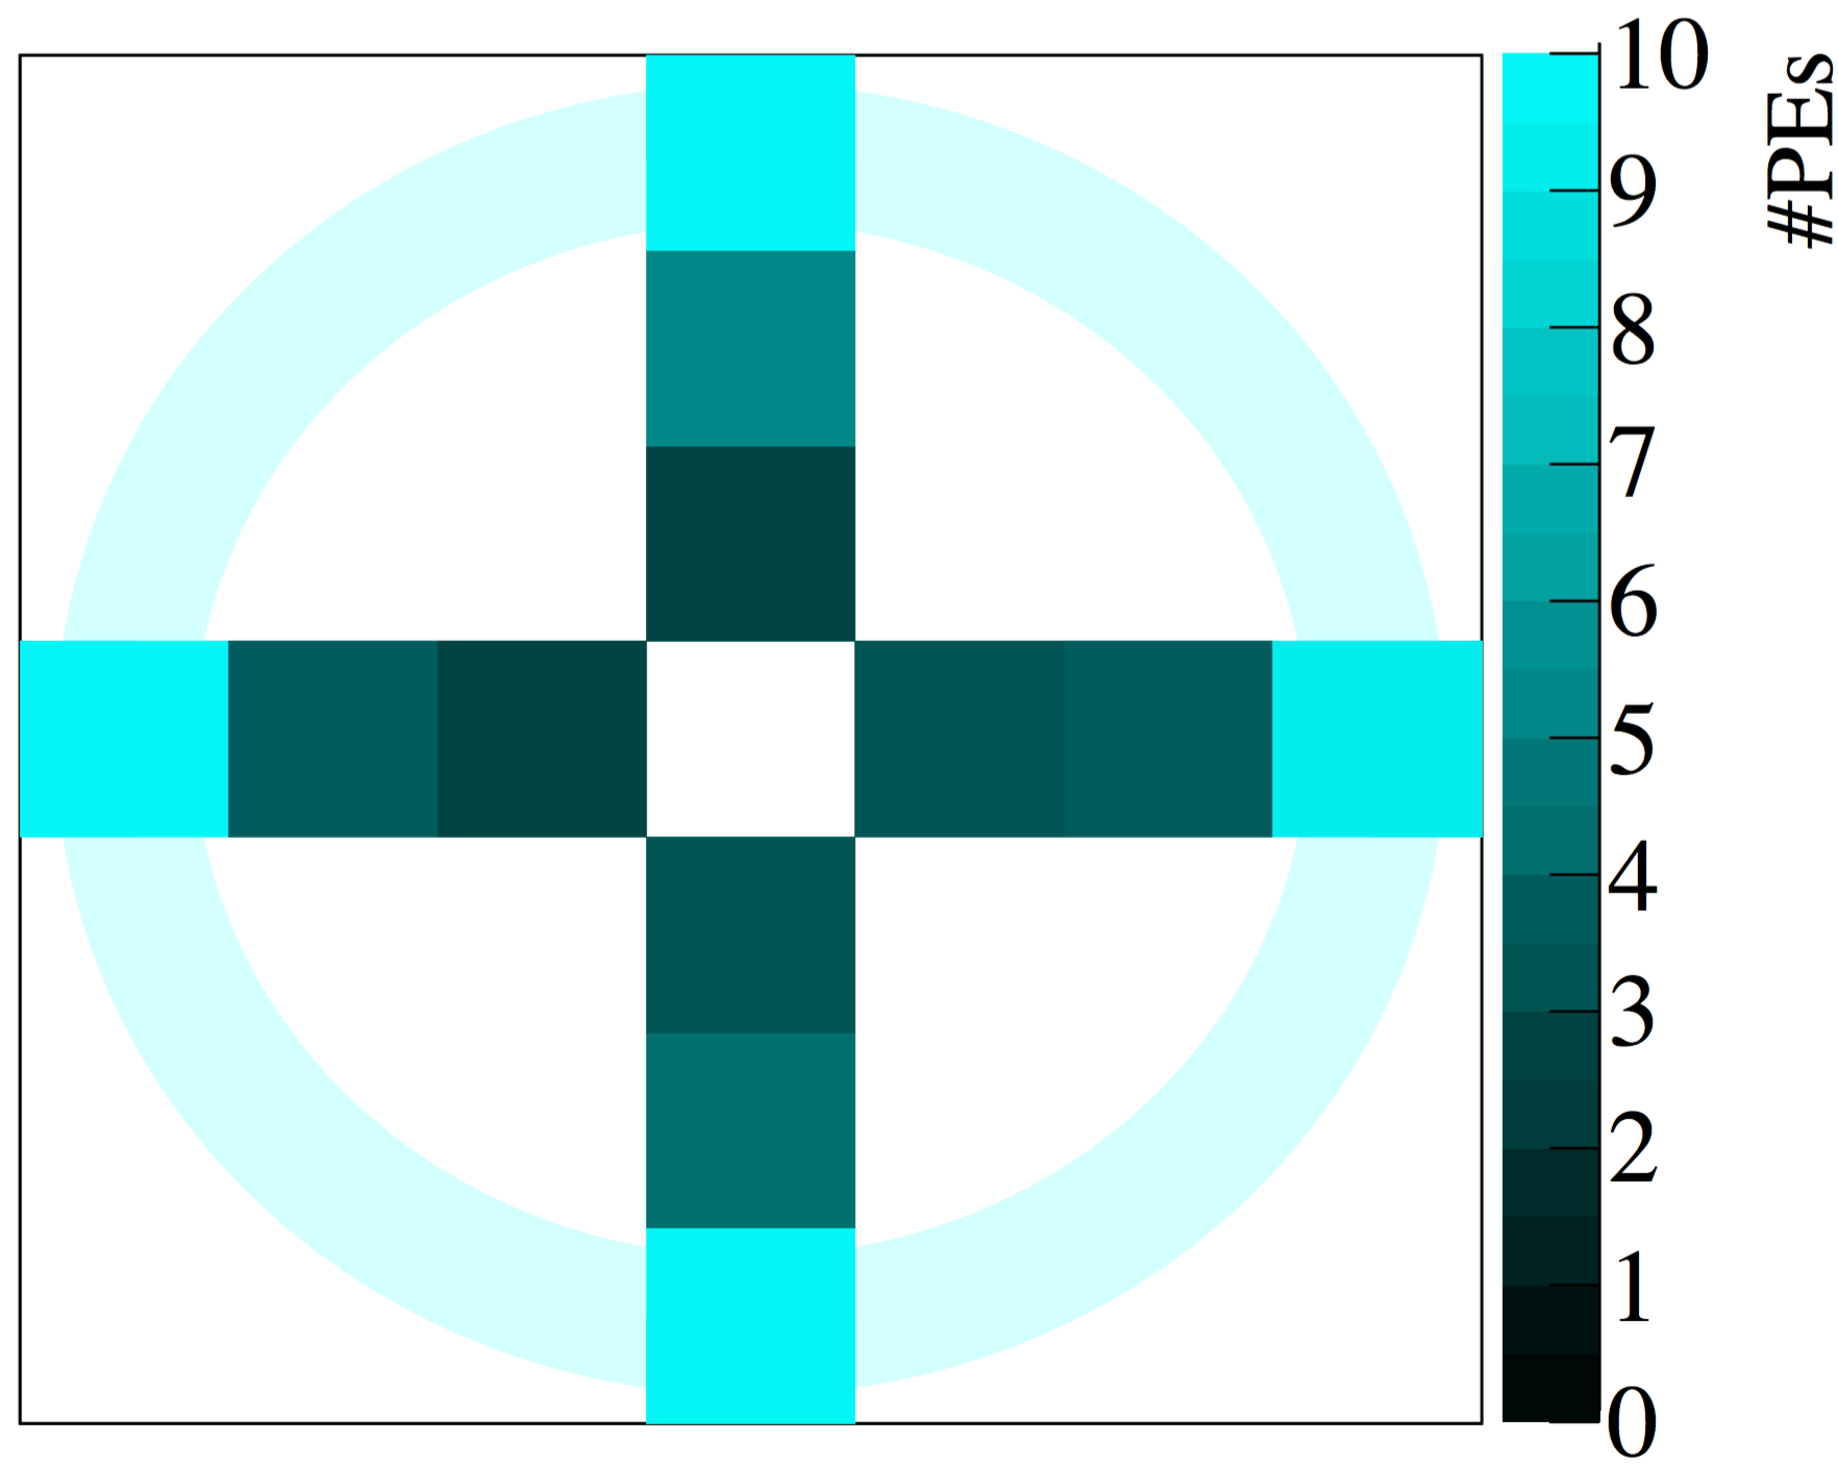
\includegraphics[width=0.47\columnwidth]{cosmic_lab_ringnpe_dt}
\caption{Average hit-time residuals (left) and average number of PE versus PMT position (right) for ring candidate events in LAB. Figure from~\cite{chess_lab}.}
\label{fig:lab2}
\end{figure}


The hit-time residual distributions for LAB are shown in \Cref{fig:lab} individually for the three radial PMT groupings, for data and MC. 
Unlike water, the larger refractive index of scintillators means that the Cherenkov photons should now fall on the outer grouping of PMTs.
The outer PMTs register the earliest hits, while the distributions for the middle and inner groups are broader and peak later, consistent with the slower scintillation light component. 
MC indicates that the early features in the inner and middle PMT groups are primarily due to Cherenkov light contamination from secondary electrons not removed by the event selection criteria.
The MC reproduces data well, supporting the conclusion that true Cherenkov / scintillation separation has been observed. 

The optimal timing cut for LAB is $ t_c = 0.4$~ns,  yielding $83\pm2$(stat.)$\pm2$(syst.)\% Cherenkov detection efficiency, with contamination of $11\pm1$(stat.)$\pm0$(syst.)\%. 
Better separation might be achieved by eliminating the Cherenkov contamination in the inner and middle PMTs via improvements to CHESS.

\begin{figure}
\centering
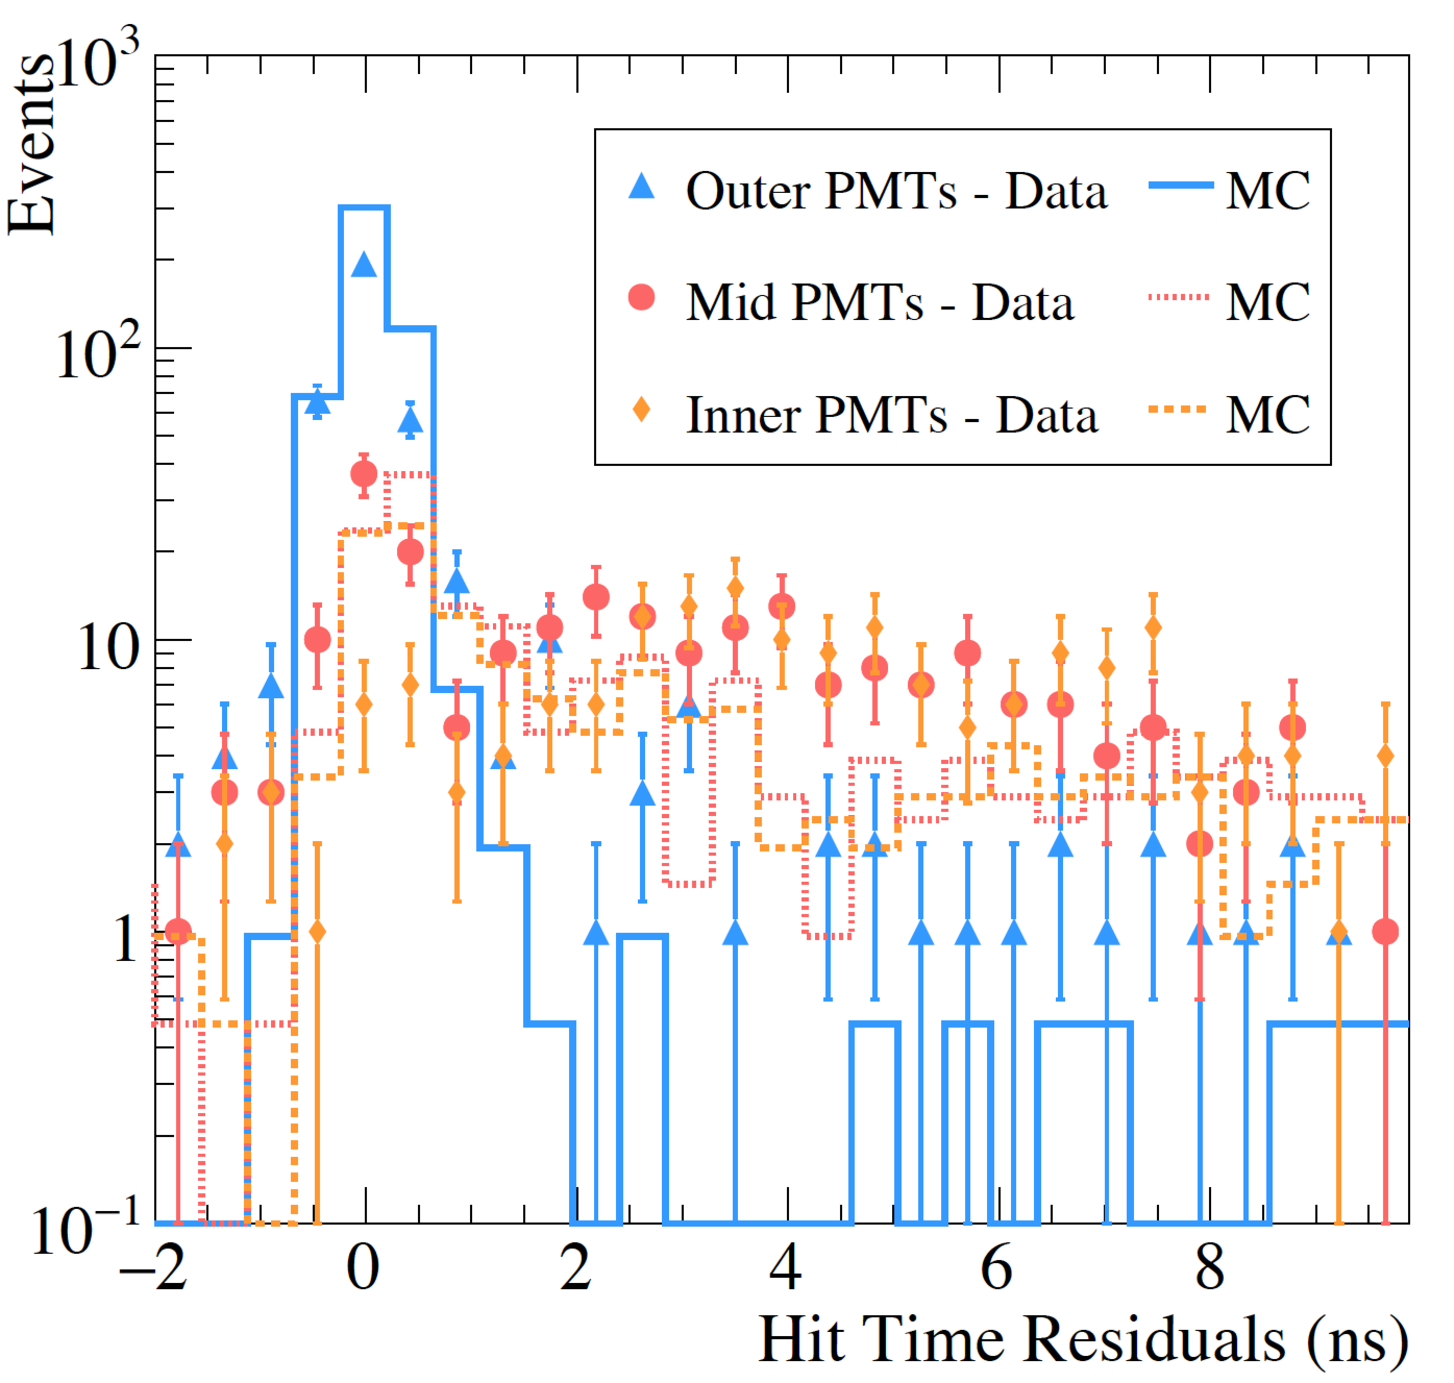
\includegraphics[width=0.7\columnwidth]{cosmic_lab_time_smear}
\caption{Hit-time residual distributions in LAB for data and MC. Figure from~\cite{chess_lab}.}
\label{fig:lab}
\end{figure}

\Cref{f:labQ} shows threshold of $Q_{\rm ratio}=0.09$ gives a Cherenkov detection efficiency of $96\pm2$(stat.)$\pm0$(syst.)\% with contamination of $6\pm3$(stat.)$\pm0$(syst.)\%.

\begin{figure}
\centering
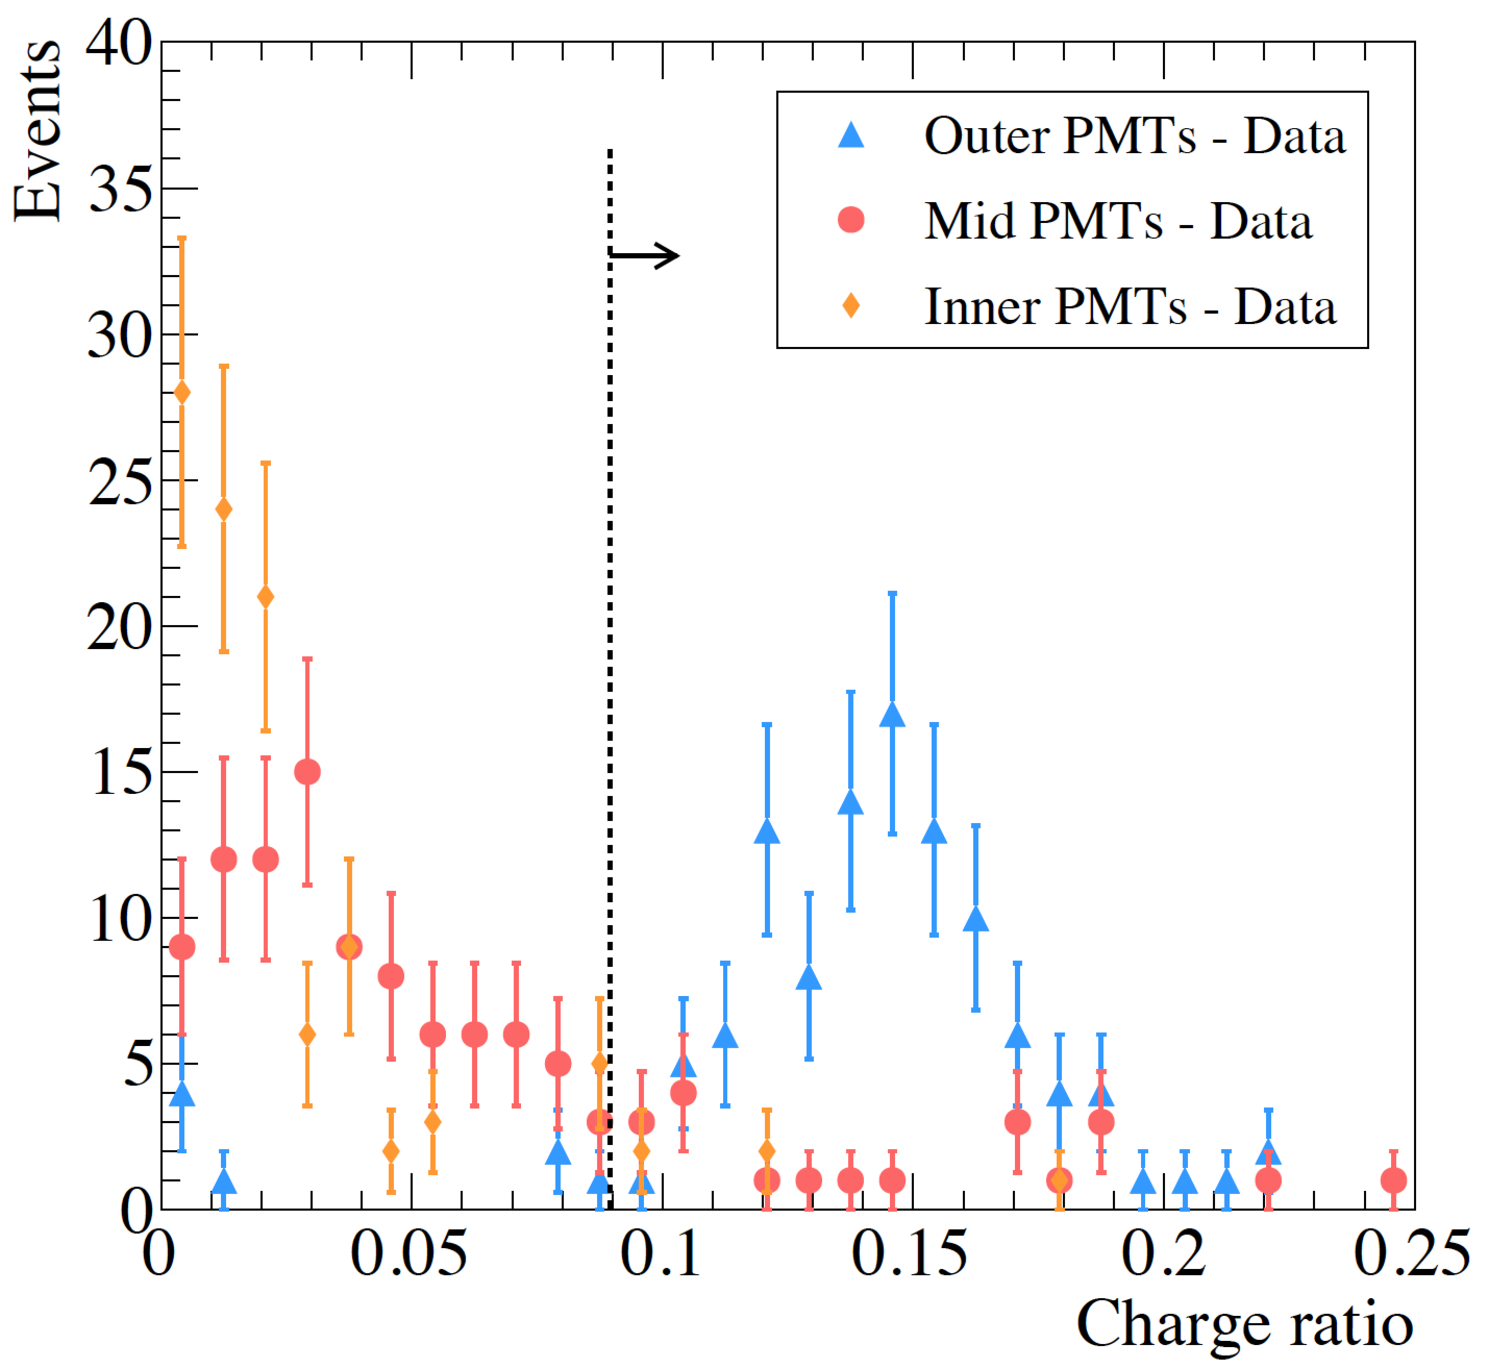
\includegraphics[width=0.7\columnwidth]{cosmic_lab_qratio5ns_led_dt}
\caption{Ratio of charge in a prompt, 5~ns window to the total charge for each hit PMT  for pure LAB. Figure from~\cite{chess_lab}.}
\label{f:labQ}
\end{figure}

\clearpage

\section{\texorpdfstring{\labppo}{LAB+PPO} Results}
\label{sec:labppo}

With Cherenkov ring-imaging demonstrated in water and pure LAB, an {\labppo} target was then deployed.
After applying event selection criteria, $103$ ring candidates were identified in the {\labppo} dataset. 
The scintillation component of {\labppo} is far too bright to identify remaining Cherenkov photons based on an intensity metric, so only the time separation metric is expected to show good results here.
Like LAB, the Cherenkov photons from {\labppo} should fall on the outermost PMTs.
The topology of a typical event, and the average across the dataset, are shown in \Cref{fig:labppo_ring}.  Again a clear ring structure can be observed. 
\begin{figure}
\centering
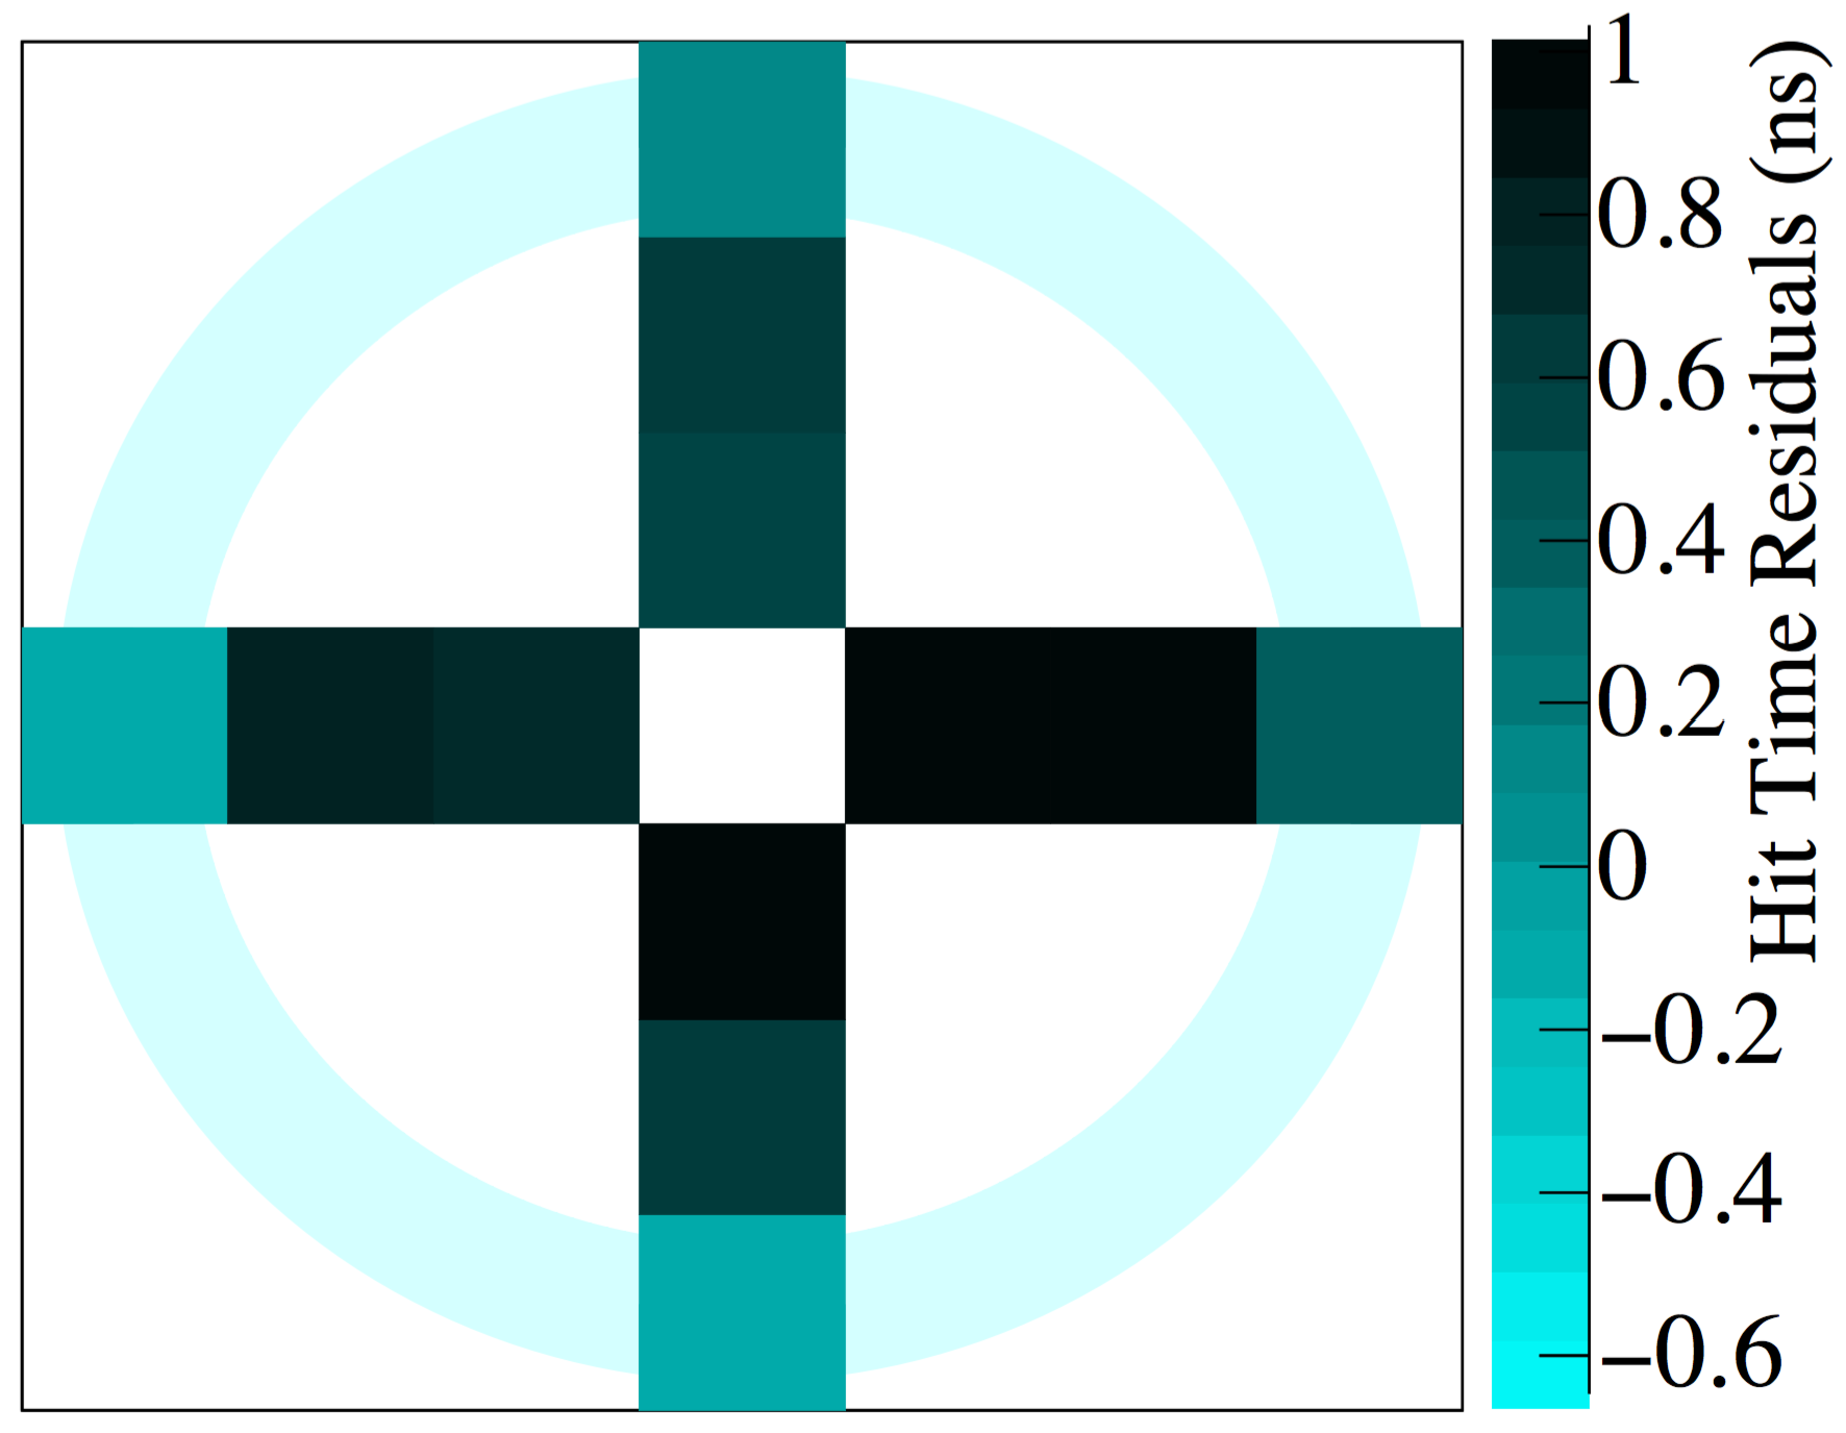
\includegraphics[width=0.47\columnwidth]{cosmic_labppo_ringcandidate_time_dt}
\hfill
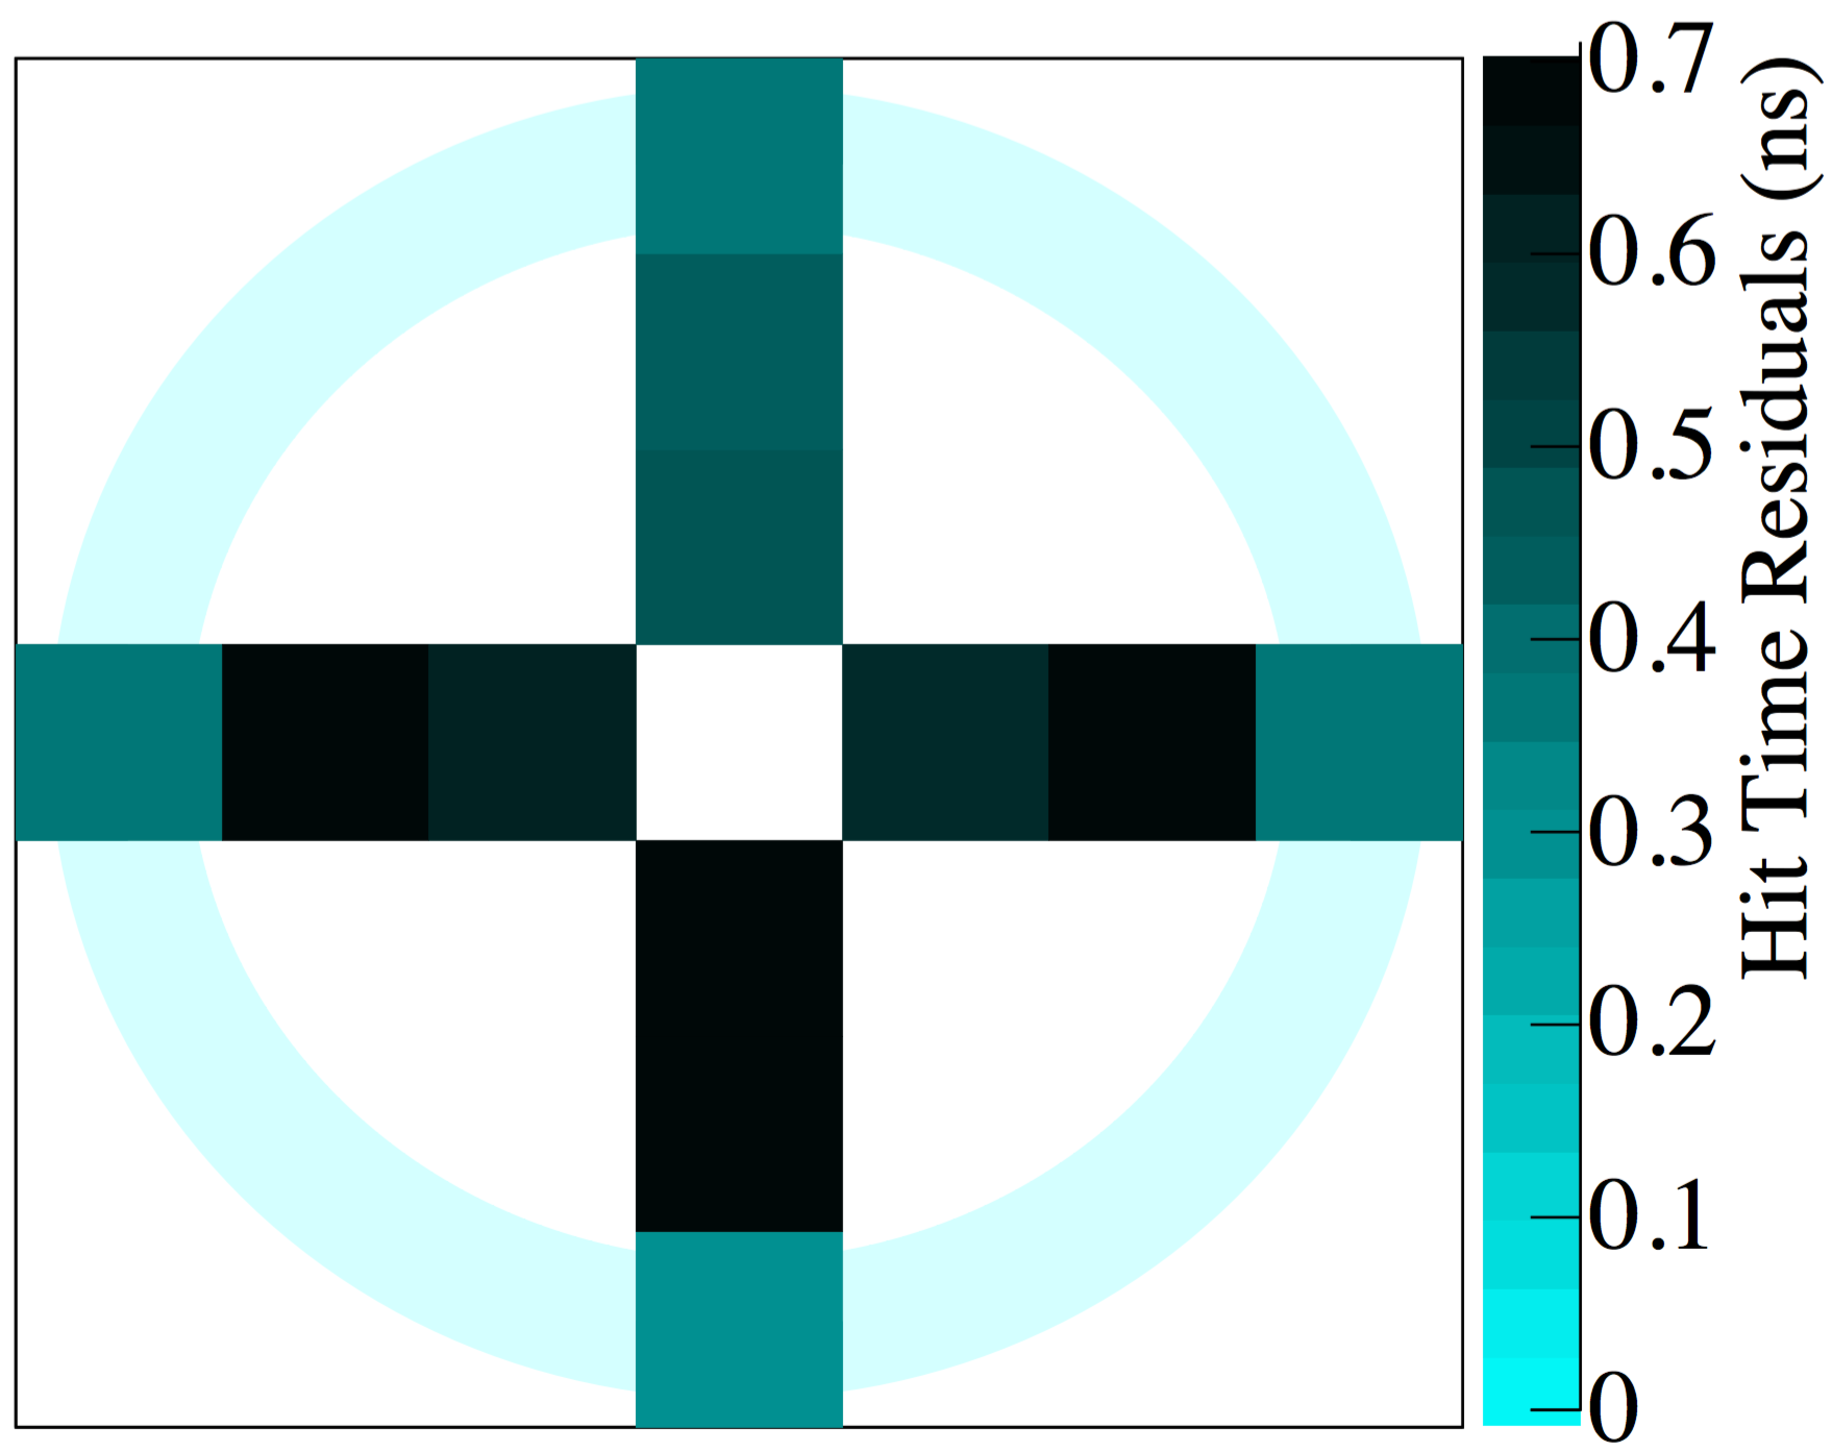
\includegraphics[width=0.47\columnwidth]{cosmic_labppo_ringtime_dt}	
\caption{Hit-time residuals versus PMT position for a single ring candidate event (left) and the average across all events (right) in {\labppo}. Figure from~\cite{chess_lab}.}
\label{fig:labppo_ring}
\end{figure}
Hit-time residual distributions are shown in \Cref{fig:labppo}, where the early Cherenkov hits on outer PMTs are clear. 
The separation is less distinct than for pure LAB.
This is expected, as the scintillation channel for pure LAB is much slower than the scintillation channel for PPO, which dominates the light output of {\labppo}.
The MC shows good agreement with data.  
A cut at $ t_c = 0.4$~ns yields Cherenkov detection efficiency of $70 \pm 3 $(stat.)$\pm0$(syst.)\% with contamination of $36 \pm 3 $(stat.)$\pm4$(syst.)\%. 

\begin{figure}
\centering
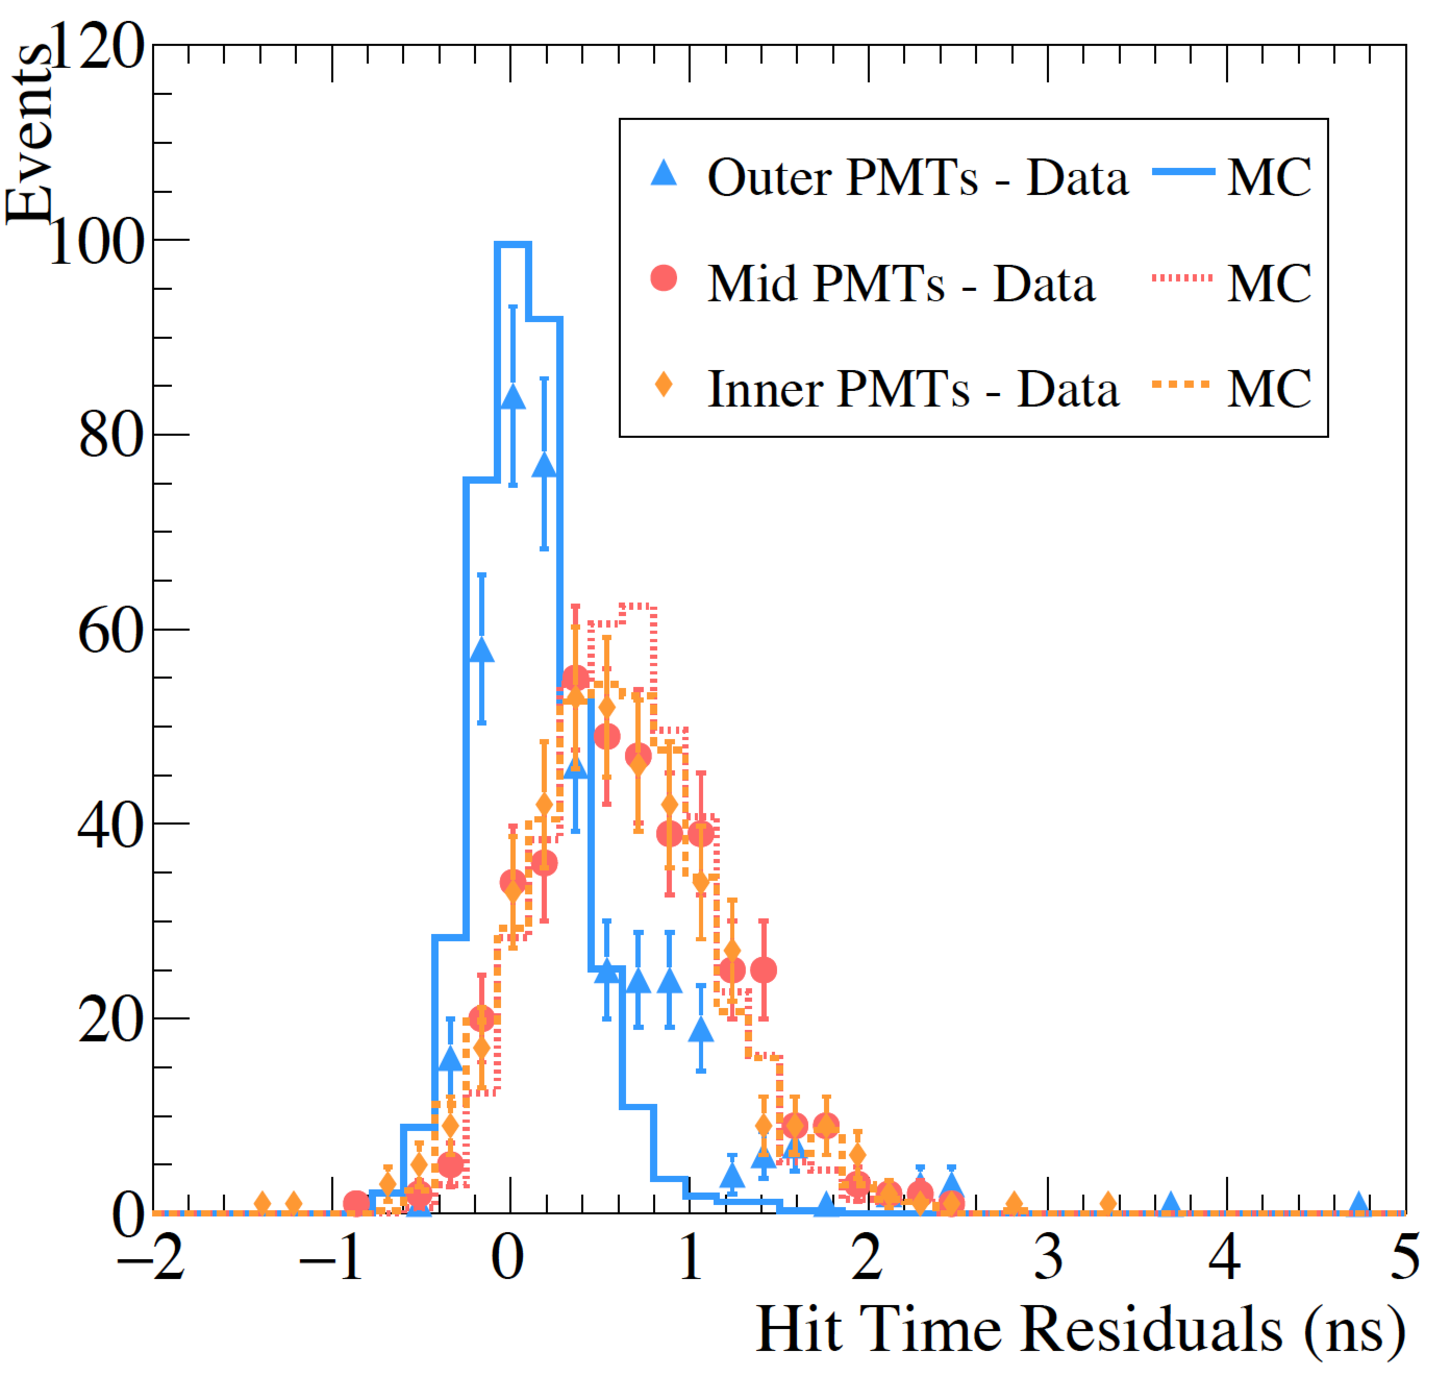
\includegraphics[width=0.7\columnwidth]{cosmic_labppo_time_smear_0p75nsrtime}
\caption{Hit-time residual distributions in {\labppo} for data and MC. Figure from~\cite{chess_lab}.}
\label{fig:labppo}
\end{figure}

The charge ratio for {\labppo} is shown in \Cref{f:labppoQ}. 
The separation is more difficult in {\labppo} due to higher scintillation yield.  
Nevertheless, a threshold of $Q_{\rm ratio}=0.038$ gives a Cherenkov detection efficiency of $63\pm4$(stat.)$\pm7$(syst.)\% with contamination of $38\pm3$(stat.)$\pm2$(syst.)\%.

\begin{figure}
\centering
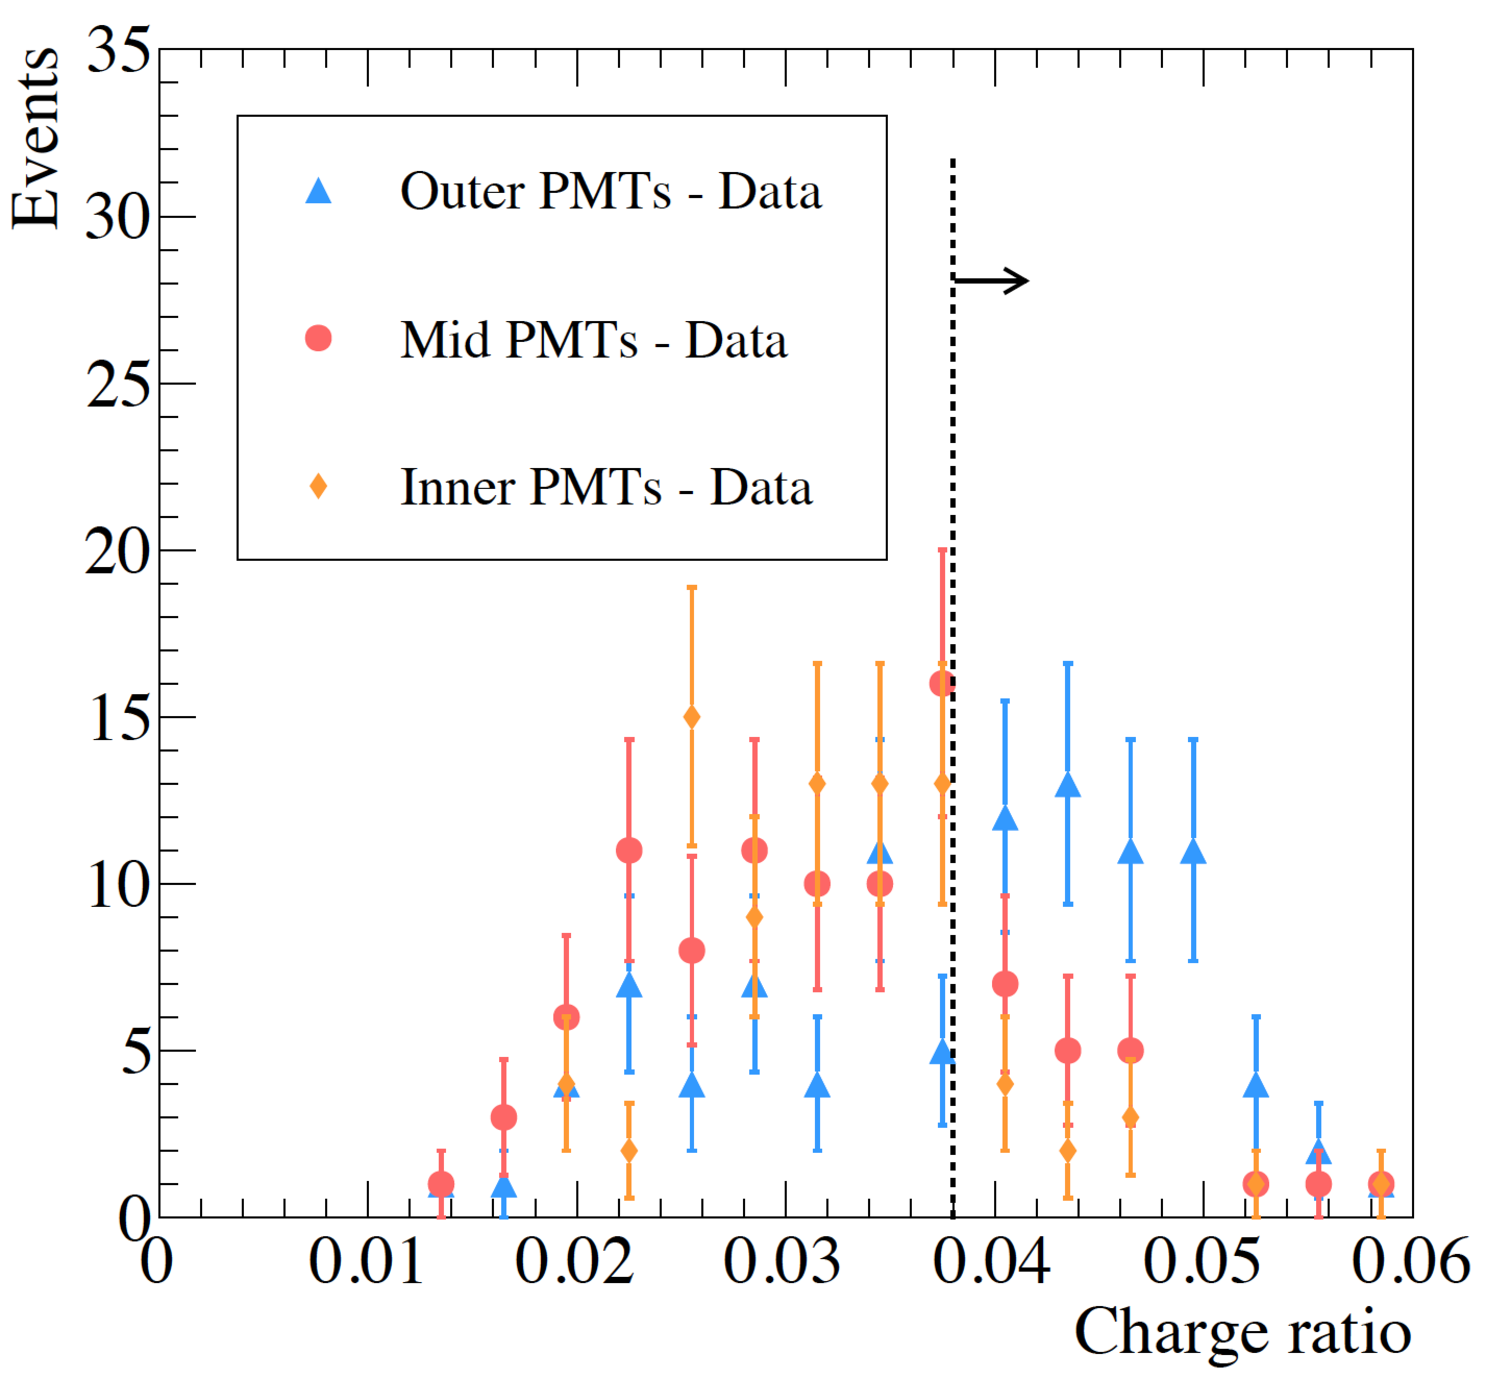
\includegraphics[width=0.7\columnwidth]{cosmic_labppo_qratio5ns_led_dt}
\caption{Ratio of charge in a prompt, 5~ns window to the total charge for each hit PMT for {\labppo}. Figure from~\cite{chess_lab}.}
\label{f:labppoQ}
\end{figure}

\clearpage

\section{Water-based Liquid Scintillator Results}
\label{sec:wbls}

Finally, CHESS was used to evaluate the Cherenkov / scintillation separation capabilities of WbLS.
Shown in this section are timing and charge results for 1\%, 5\%, and 10\% scintillator mixtures that are expected to have roughly 1\%, 5\%, and 10\% of {\labppo} light yield.
Because the scintillation component is expected to be very dim for the lower scintillator fractions, the results shown here for charge are directly in units of PE instead of the charge ratio shown for brighter LS in previous sections.
The refractive index of these low scintillator fraction WbLS materials is very similar to water, so the Cherenkov ring is expected to fall on the middle radial grouping of PMTs.

\subsection{1\% WbLS}

After applying selection criteria to the 1\% WbLS dataset, 130 ring candidates are found.
The average hit-time residuals and average charge observed by each PMT is given in \Cref{fig:wbls1pct_avg}.
In both cases, this material looks very similar to water with a dim scintillation component.
The hit-time residual distributions shown in \Cref{fig:wbls1pct_tresid} indicate a clear population of prompt Cherenkov photons on the middle grouping of PMTs.
Similarly, the total number of PE distributions shown in \Cref{fig:wbls1pct_totalq} clearly shows that the middle group of PMTs, seeing Cherenkov and scintillation photons, detect about a factor of 5 more PE than the other populations, which see only scintillation light.


\begin{figure}
\centering
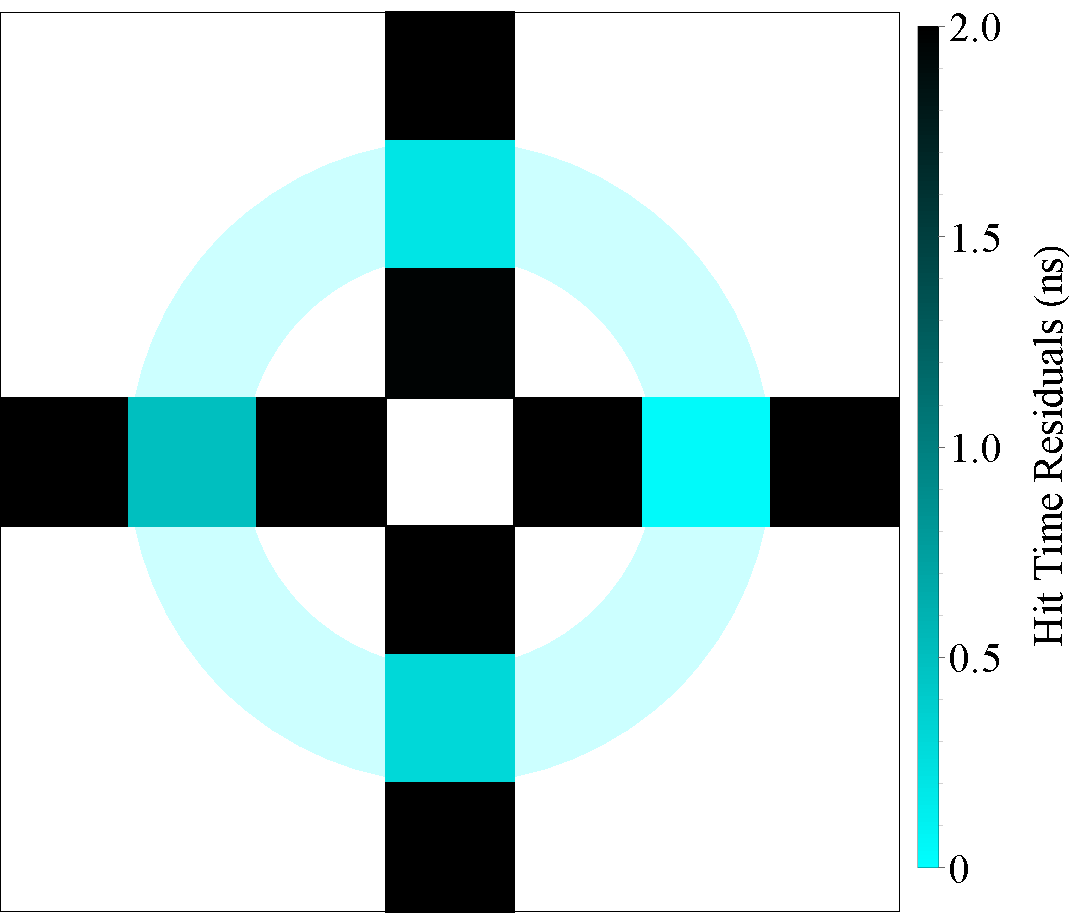
\includegraphics[width=0.47\columnwidth]{wbls_1pct_avg_time}
\hfill

\includegraphics[width=0.47\columnwidth]{wbls_1pct_avg_charge}
\caption{\label{fig:wbls1pct_avg}The average hit-time residuals (left) and average number of detected PE (right) for all selected events in the 1\% WbLS dataset.}
\end{figure}

\begin{figure}
\centering
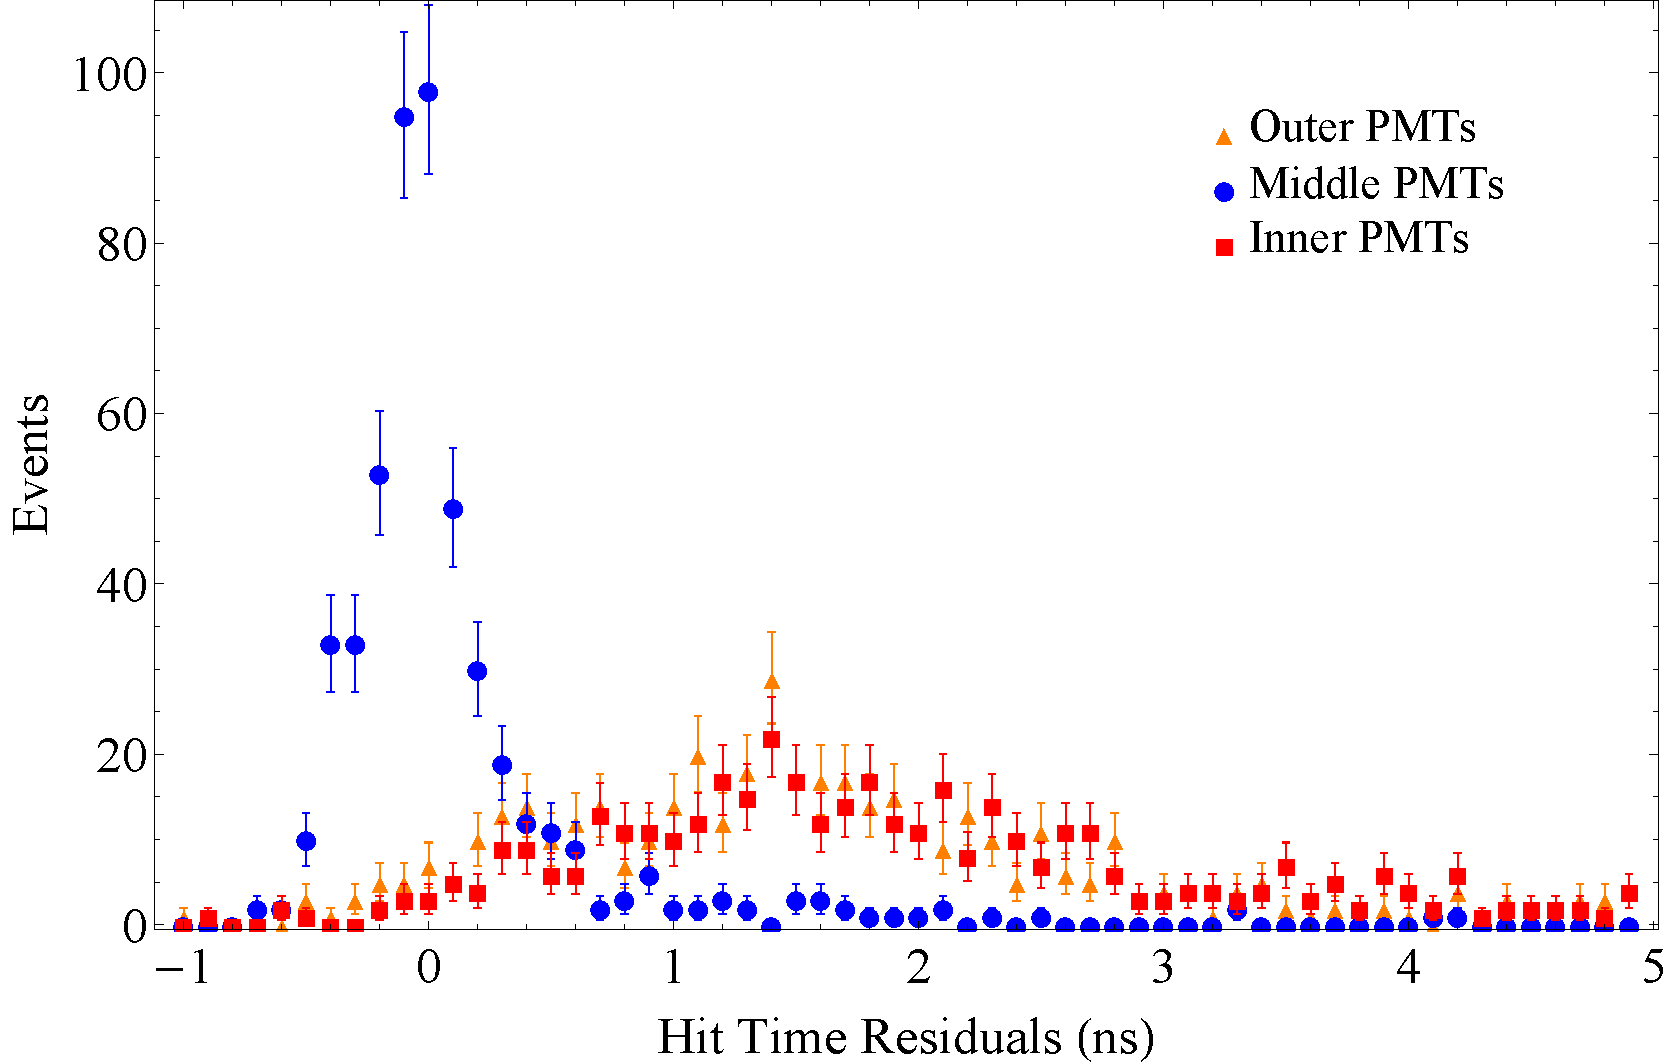
\includegraphics[width=0.8\columnwidth]{wbls_1pct_hittimes}
\caption{\label{fig:wbls1pct_tresid}A histogram of the hit-time residuals for all selected events in the 1\% WbLS dataset grouped by PMT radius.}
\end{figure}

\begin{figure}
\centering
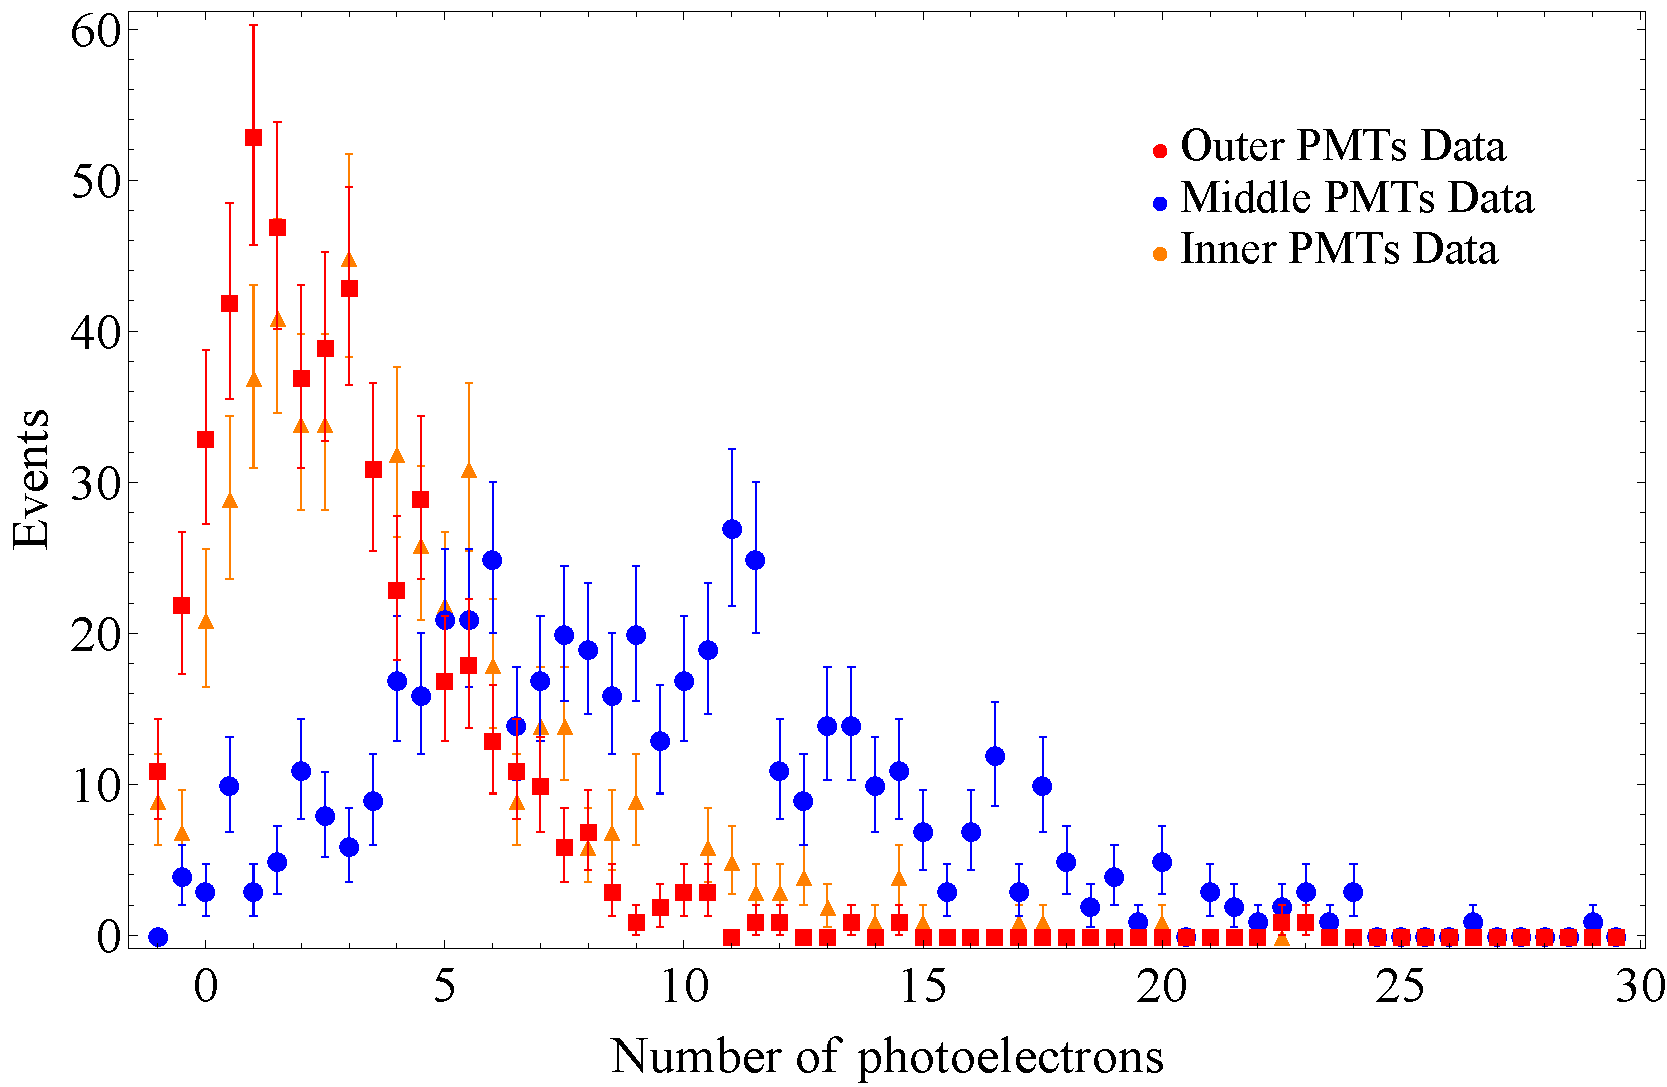
\includegraphics[width=0.8\columnwidth]{wbls_1pct_charge}
\caption{\label{fig:wbls1pct_totalq}A histogram of the total number of PE for all selected events in the 1\% WbLS dataset grouped by PMT radius.}
\end{figure}

\clearpage

\subsection{5\% WbLS}

After applying selection criteria to the 5\% WbLS dataset, 83 ring candidates are found.
The average hit-time residuals and average charge observed by each PMT is given in \Cref{fig:wbls5pct_avg}.
Relative to the 1\% WbLS results, the scintillation component is notably brighter, resulting in a poorer contrast in charge.
The hit-time residual distributions shown in \Cref{fig:wbls5pct_tresid} still indicate a clear population of prompt Cherenkov photons on the middle grouping of PMTs, meaning time-based separation is still viable.
The total number of PE distributions shown in \Cref{fig:wbls5pct_totalq} indicate charge based separation will be more difficult than 1\% WbLS.
The middle group of PMTs does observe a slightly higher number of PE on average, so there is potential for Cherenkov photon detection via intensity.

\begin{figure}
\centering
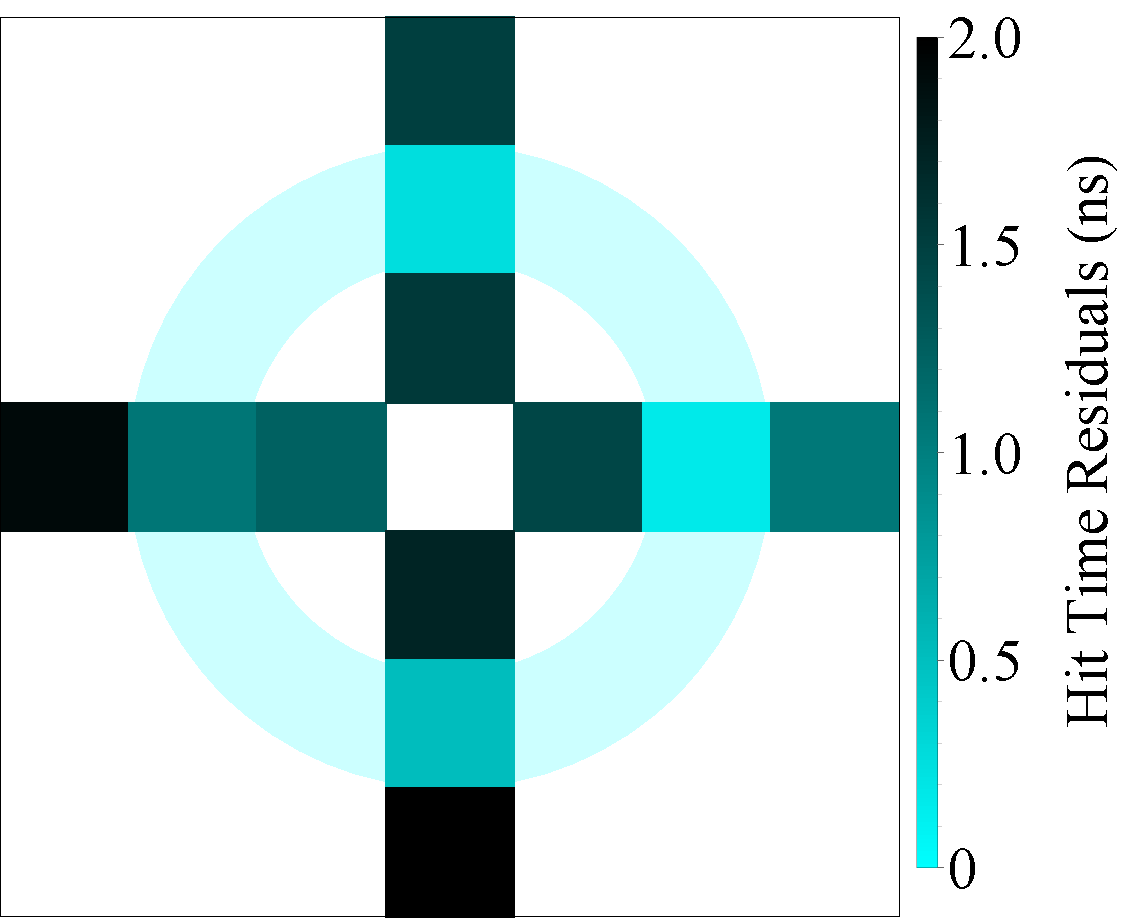
\includegraphics[width=0.47\columnwidth]{wbls_5pct_avg_time}
\hfill
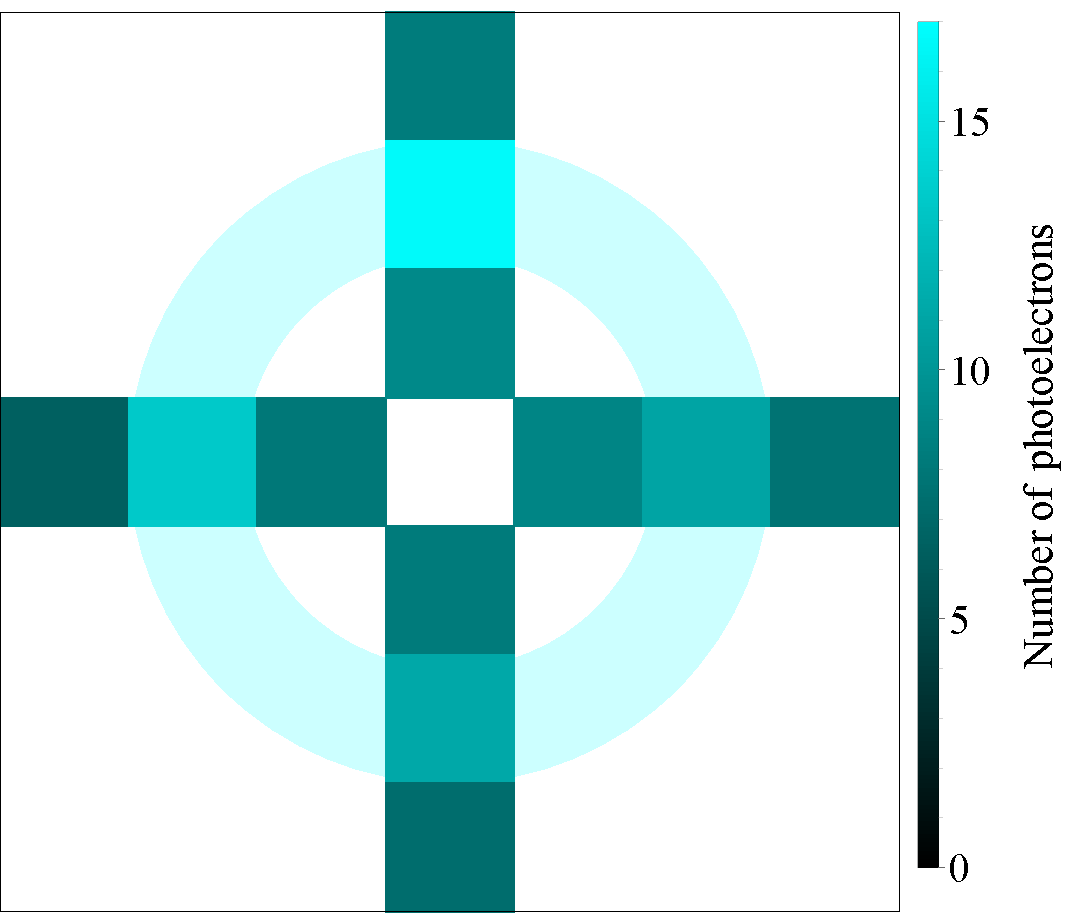
\includegraphics[width=0.47\columnwidth]{wbls_5pct_avg_charge}
\caption{\label{fig:wbls5pct_avg}The average hit-time residuals (left) and average number of detected PE (right) for all selected events in the 5\% WbLS dataset.}
\end{figure}

\begin{figure}
\centering
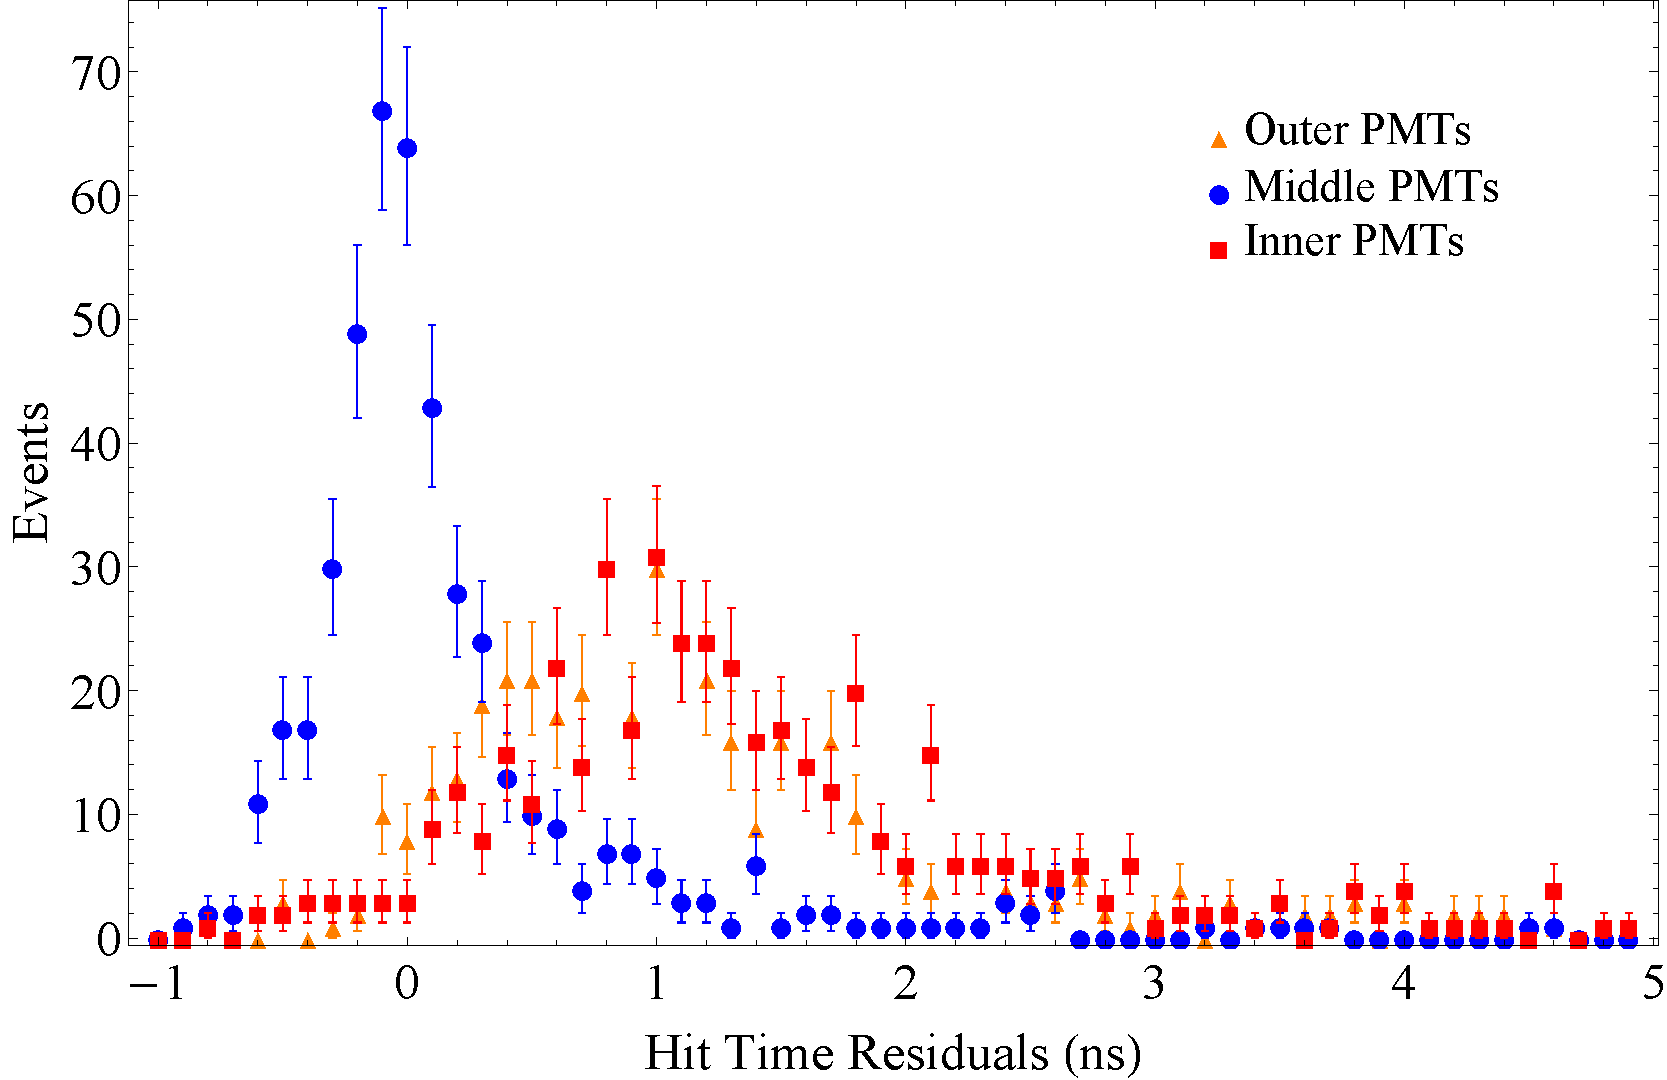
\includegraphics[width=0.8\columnwidth]{wbls_5pct_hittimes}
\caption{\label{fig:wbls5pct_tresid}A histogram of the hit-time residuals for all selected events in the 5\% WbLS dataset grouped by PMT radius.}
\end{figure}

\begin{figure}
\centering
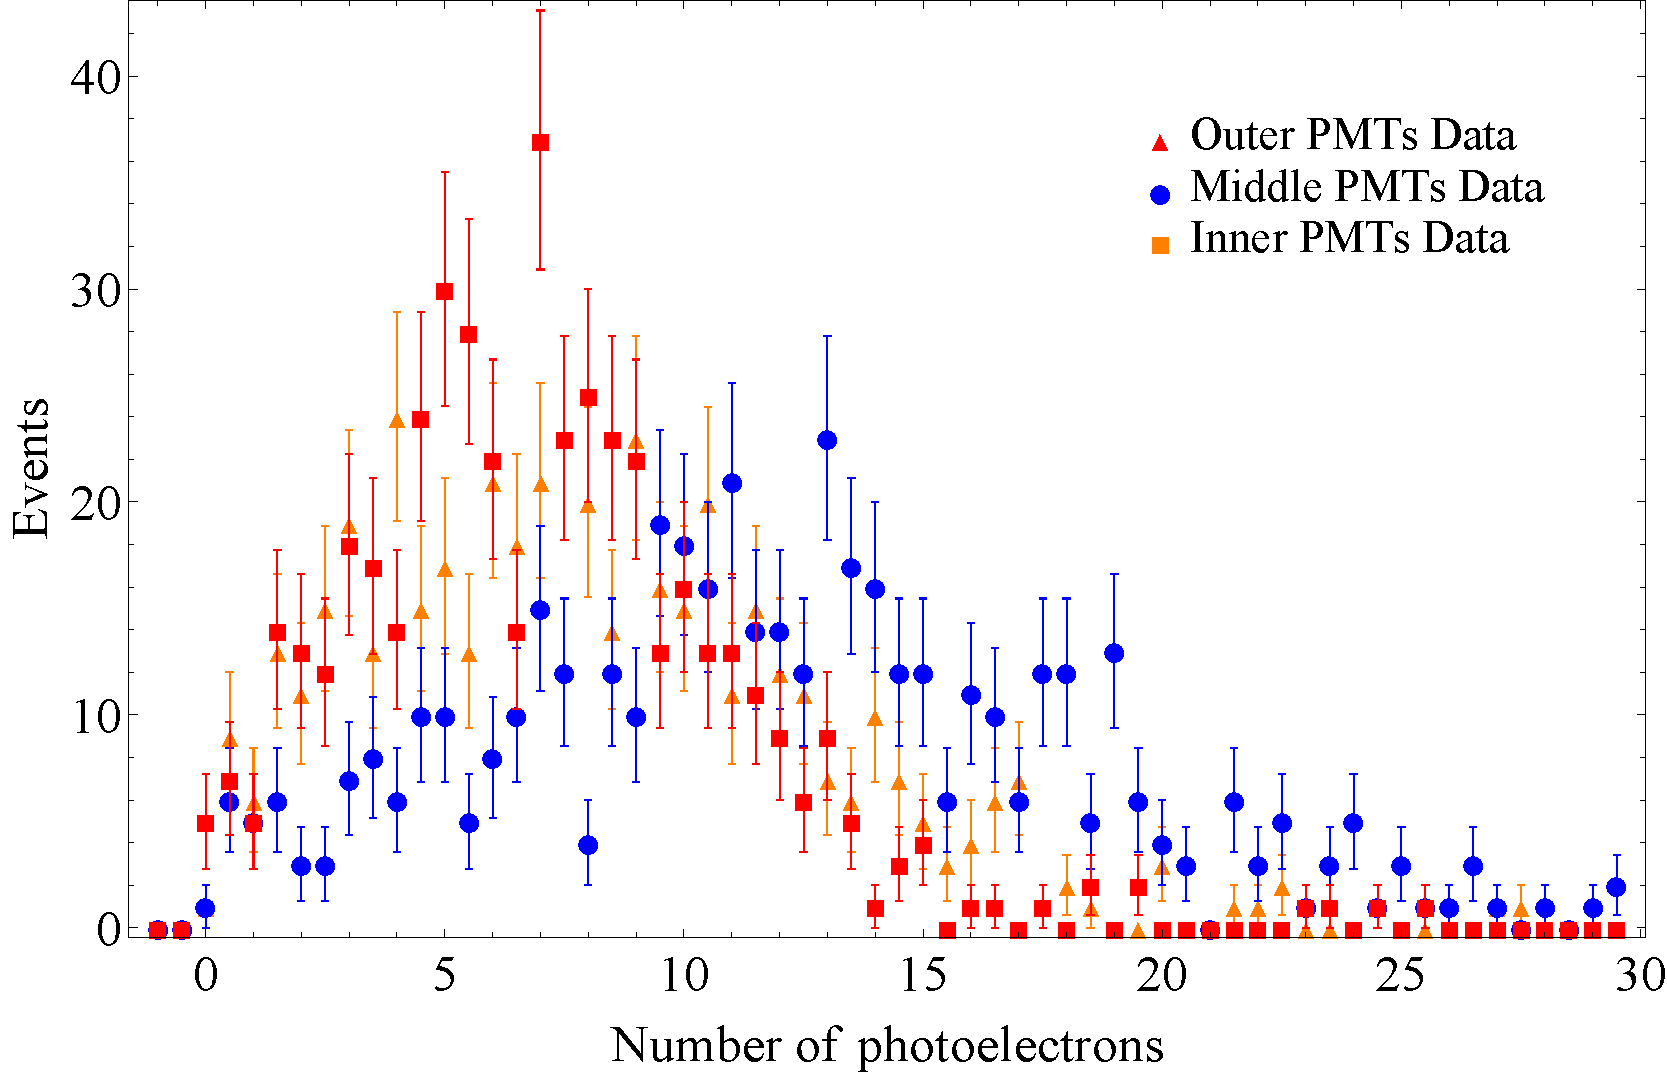
\includegraphics[width=0.8\columnwidth]{wbls_5pct_charge}
\caption{\label{fig:wbls5pct_totalq}A histogram of the total number of PE for all selected events in the 5\% WbLS dataset grouped by PMT radius.}
\end{figure}

\clearpage

\subsection{10\% WbLS}

After applying selection criteria to the 10\% WbLS dataset, 171 ring candidates are found.
The average hit-time residuals and average charge observed by each PMT is given in \Cref{fig:wbls10pct_avg}.
Here the scintillation component is now bright enough that the contrast between the Cherenkov and scintillation regions in intensity is quite poor.
The hit-time residual distributions shown in \Cref{fig:wbls10pct_tresid} are not that dissimilar from the 5\% WbLS results, with a clear prompt Cherenkov signal on the middle PMTs.
The total number of PE distributions shown in \Cref{fig:wbls10pct_totalq} reveal a slight upward shift in the charge of the middle PMTs compared to the width of the distribution.
Identification of individual Cherenkov photons based purely on intensity would be a challenge, but statistical identification of the ring may still offer some handle for direction reconstruction.

\begin{figure}
\centering
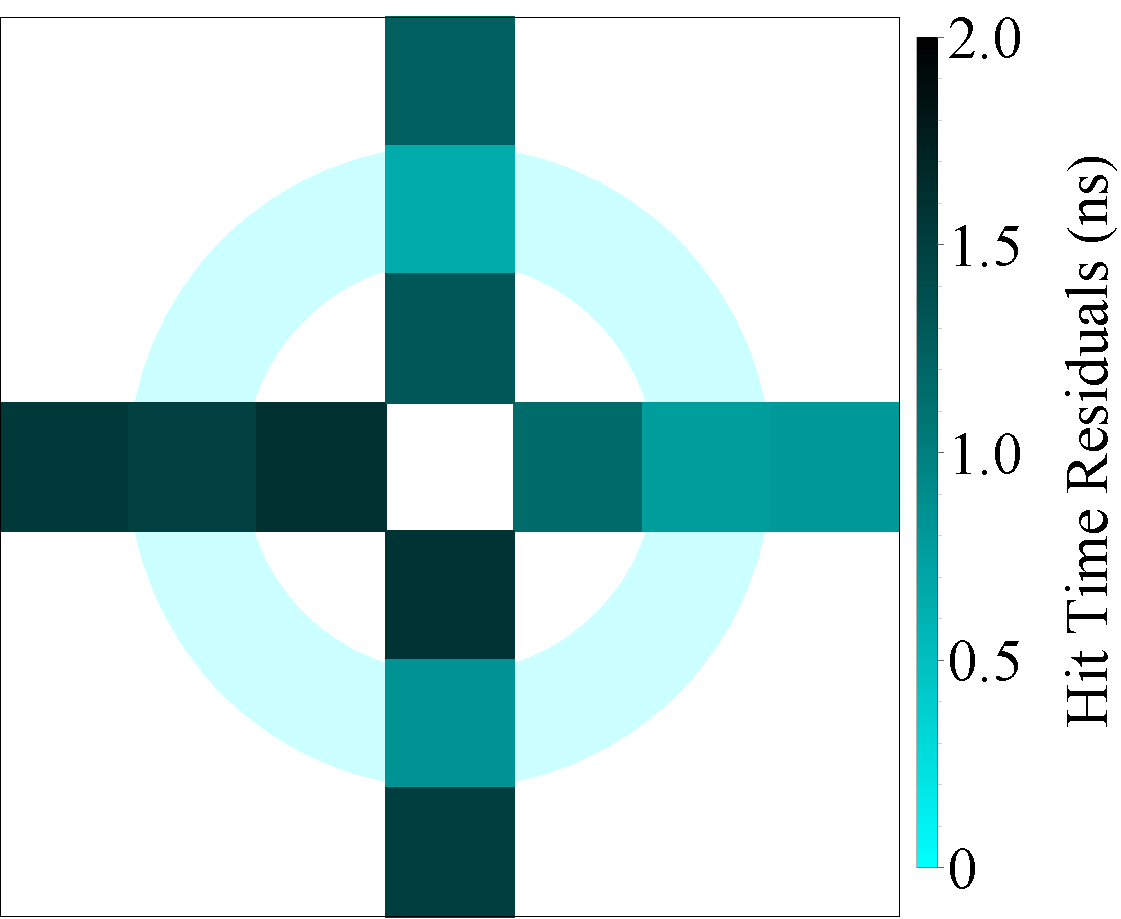
\includegraphics[width=0.47\columnwidth]{wbls_10pct_avg_time}
\hfill
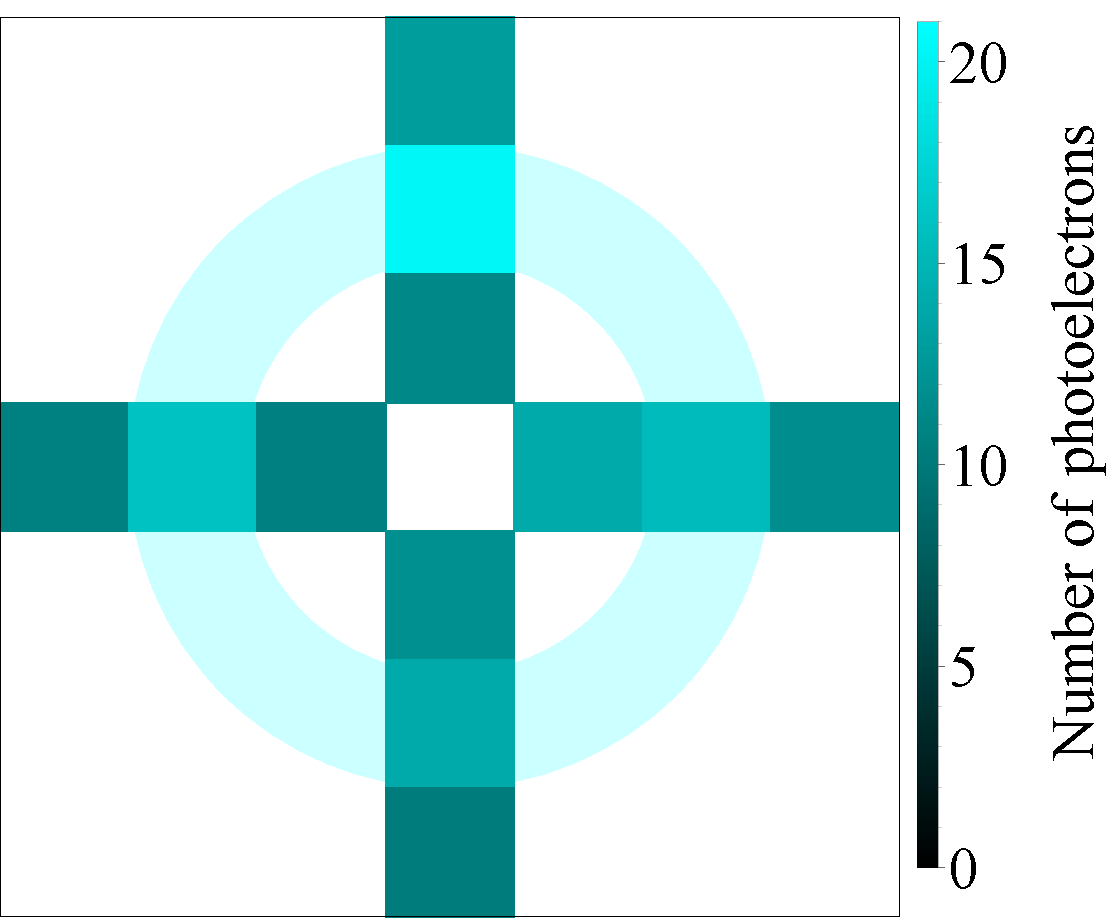
\includegraphics[width=0.47\columnwidth]{wbls_10pct_avg_charge}
\caption{\label{fig:wbls10pct_avg}The average hit-time residuals (left) and average number of detected PE (right) for all selected events in the 10\% WbLS dataset.}
\end{figure}

\begin{figure}
\centering
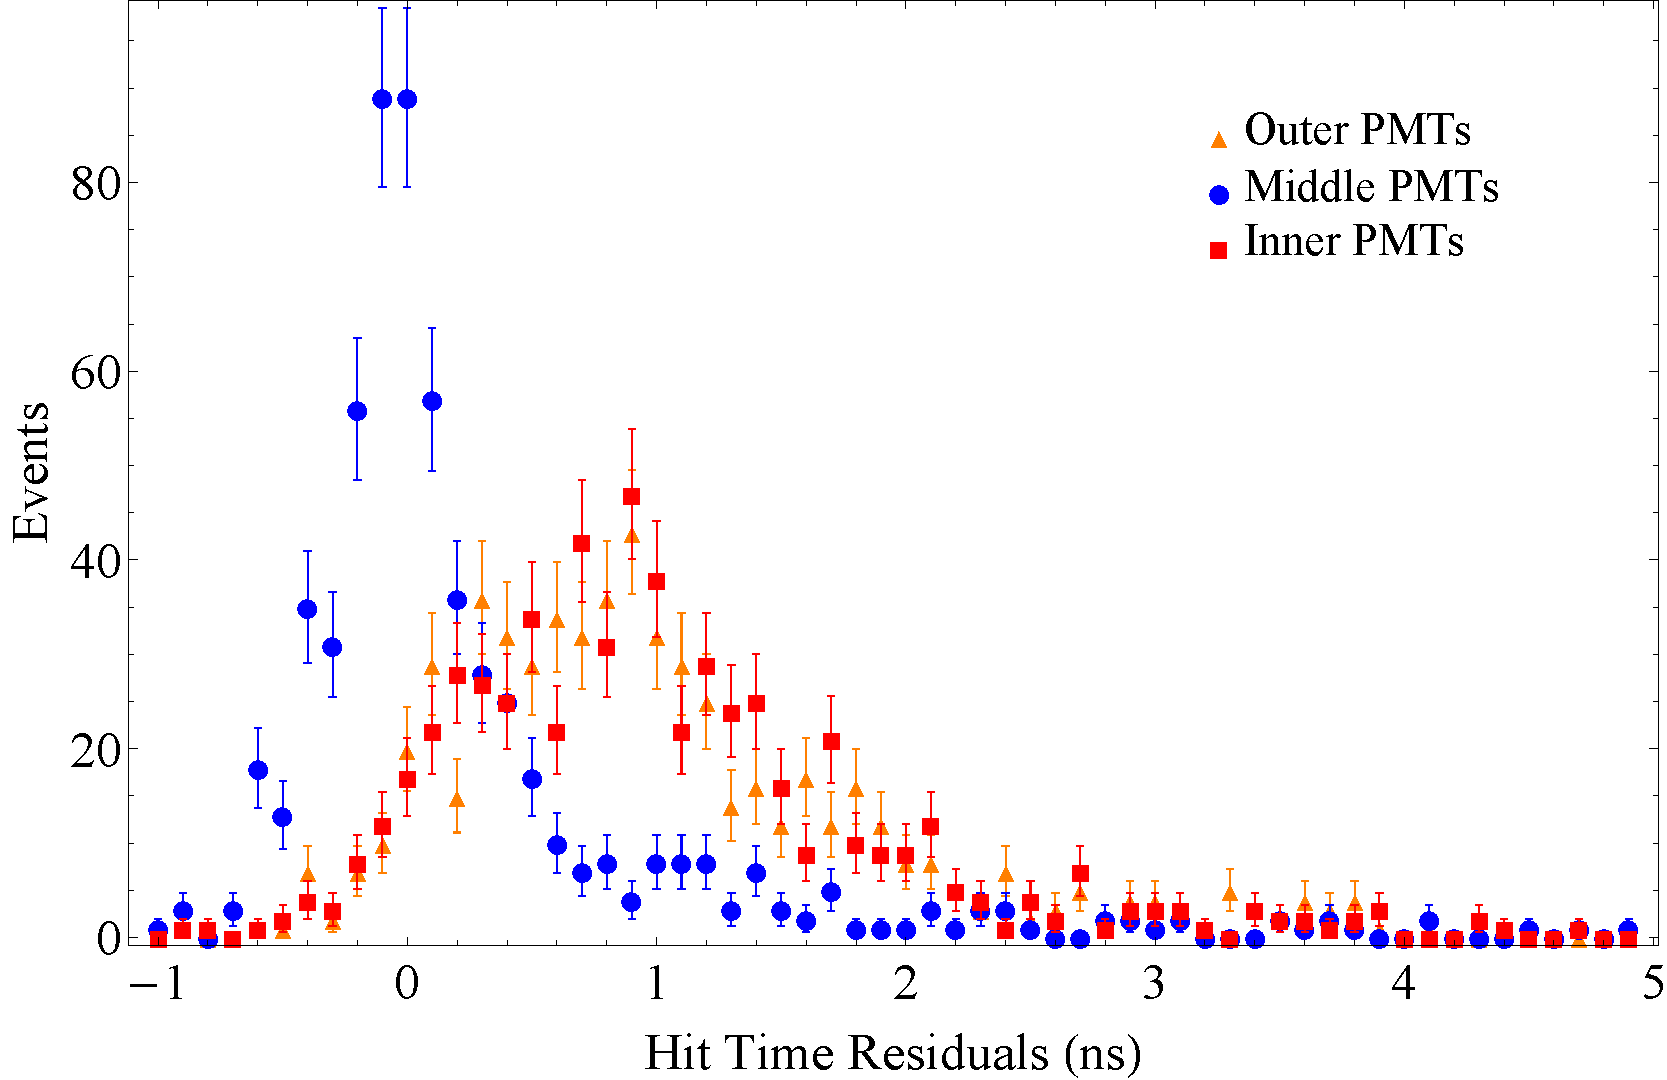
\includegraphics[width=0.8\columnwidth]{wbls_10pct_hittimes}
\caption{\label{fig:wbls10pct_tresid}A histogram of the hit-time residuals for all selected events in the 10\% WbLS dataset grouped by PMT radius.}
\end{figure}

\begin{figure}
\centering
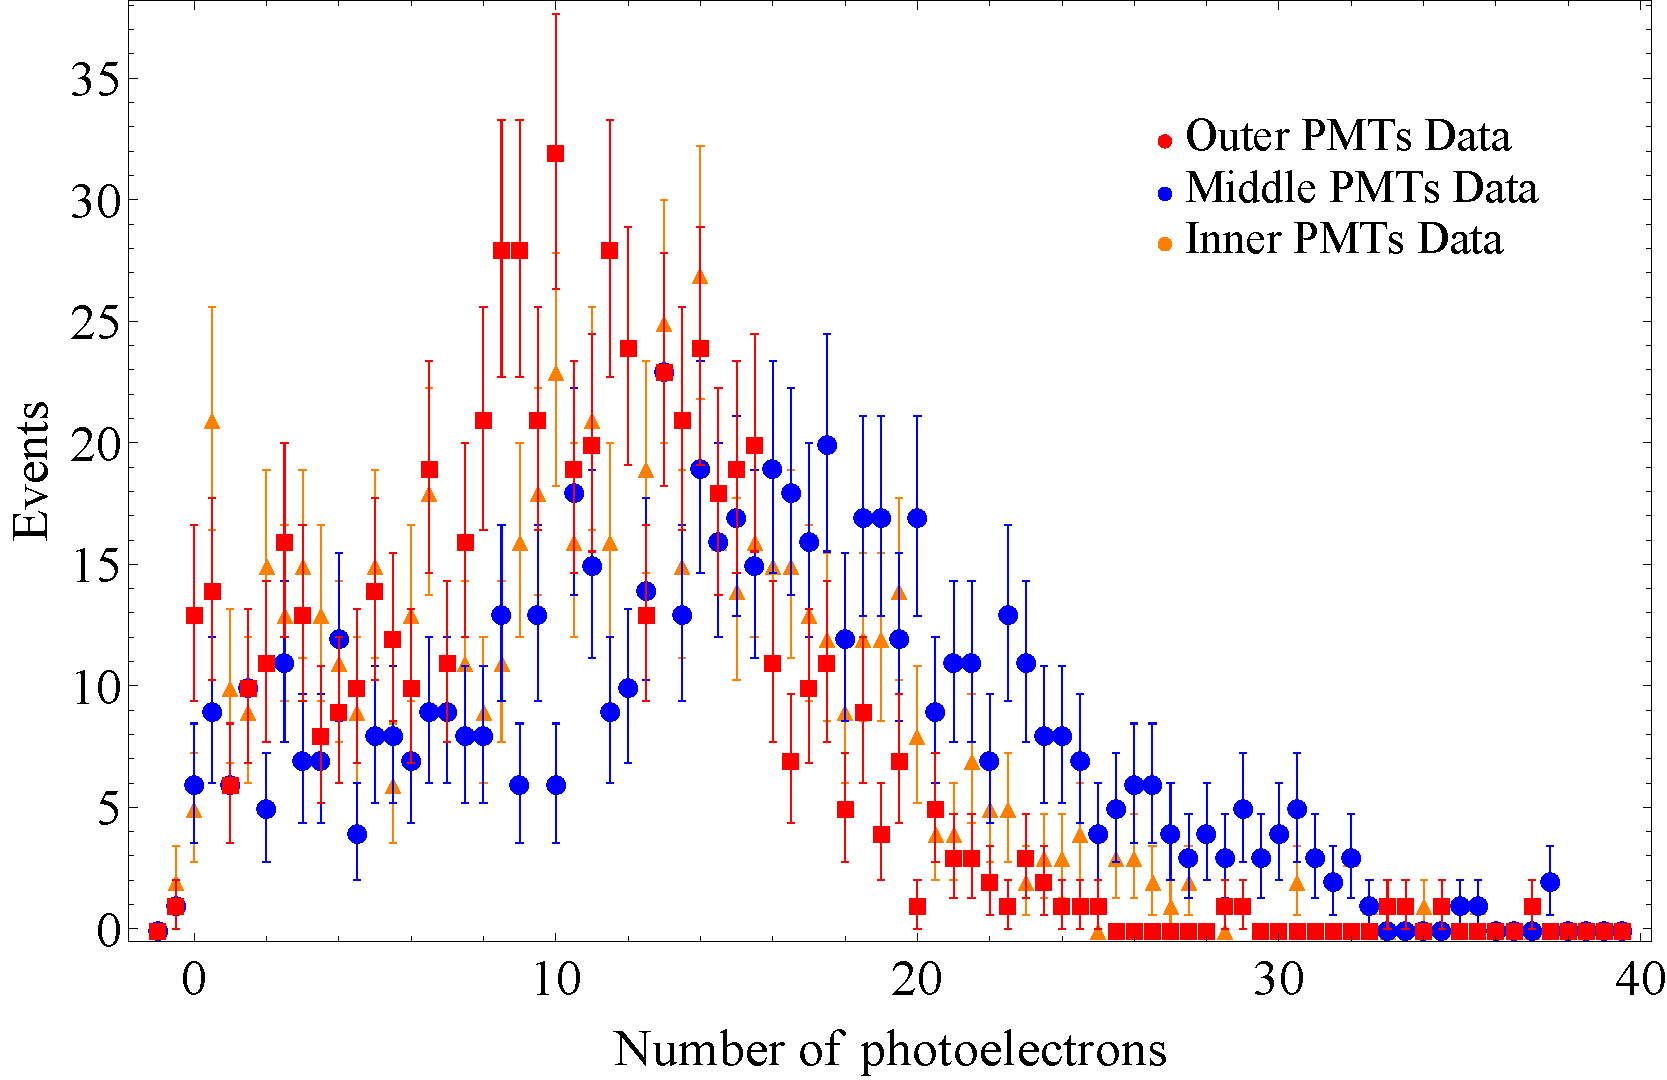
\includegraphics[width=0.8\columnwidth]{wbls_10pct_charge}
\caption{\label{fig:wbls10pct_totalq}A histogram of the total number of PE for all selected events in the 10\% WbLS dataset grouped by PMT radius.}
\end{figure}

\section{Prospects}

CHESS demonstrated the potential for Cherenkov / scintillation separation in the traditional scintillator {\labppo}, with the caveat that very fast photon detectors are required.
Modern large PMTs are approaching 1~ns time resolutions, which may be sufficient to achieve a reasonably pure population of prompt Cherenkov photons to extract directional information.
Faster photon detectors are currently being developed in the form of micro-channel plate (MCP) based detectors~\cite{lappd,lappd2}, which can achieve time resolutions better than 100~ps.
While they are cost-prohibitive at the moment (compared to large PMTs), these devices have better time resolution than CHESS, and would be good candidates for time based Cherenkov / scintillation separation.

In the more immediate future, CHESS has demonstrated clear Cherenkov / scintillation separation in both intensity and time in WbLS materials with low scintillator fraction. 
The results of this small-scale test indicate that WbLS in the 1\%-5\% scintillator fraction regime should show clear separation between Cherenkov and scintillation signals in both intensity and time.
At 10\% scintillator fraction, CHESS observed similar intensity distributions for the scintillation-only and Cherenkov+scintillation PMT radial groupings, while the hit-time residual distributions were similar to lower scintillator fractions, showing good separation.
Extrapolation of this result to larger detectors, such as \textsc{Theia} is not trivial, and will require larger scale tests to properly account for scattering and attenuation effects.
However, this result does indicate low scintillator fraction WbLS materials are strong candidates for Cherenkov / scintillation separation at large scale.

Further, CHESS results show that prompt time cuts on the order of a nanosecond --- potentially achievable with existing large PMTs --- can result in a more pure sample of Cherenkov photons than would be achievable without timing information.
As new photodetectors with better time resolution become available, time separation will be able to further purify the sample of Cherenkov photons.
A purer sample of Cherenkov photons would make intensity-based identification of Cherenkov topology easier, especially in the case of scintillator fractions greater than 10\%, and potentially extending to pure scintillators like {\labppo}.
This synergy between intensity and timing information should be leveraged in further studies of Cherenkov / scintillation separation.
